\documentclass[12pt, a4paper, oneside, openright, titlepage]{book}
\usepackage[utf8]{inputenc}
\raggedbottom
\usepackage{import}


%%%%%%%%%%%%%%%%% Book Formatting Comments:

%%%%%%%%%%%%%%%%%%%%%%%%%%%%%%%%%%%%% for Part

%%%%%%%%%%%%%%%%%%%%%% for chapter

%%%%%%%%%%%%%%%%%%%% for section




%%%%%% PACKAGES %%%%%%%
\usepackage{hyperref}
\hypersetup{
    colorlinks,
    citecolor=black,
    filecolor=black,
    linkcolor=black,
    urlcolor=black
}
\usepackage{amsmath} % Math display options
\usepackage{amssymb} % Math symbols
%\usepackage{amsfonts} % Math fonts
%\usepackage{amsthm}
\usepackage{mathtools} % General math tools
\usepackage{array} % Allows you to write arrays
\usepackage{empheq} % For boxing equations
% \usepackage{mathabx}
% \usepackage{mathrsfs}
\usepackage{nameref}
\usepackage{wrapfig}

\usepackage{soul}
\usepackage[normalem]{ulem}

\usepackage{txfonts}
\usepackage{cancel}
\usepackage[toc, page]{appendix}
\usepackage{titletoc,tocloft}
\setlength{\cftchapindent}{1em}
\setlength{\cftsecindent}{2em}
\setlength{\cftsubsecindent}{3em}
%\setlength{\cftsubsubsecindent}{4em}
\usepackage{titlesec}

%\titleformat{\section}
%  {\normalfont\fontsize{25}{15}\bfseries}{\thesection}%{1em}{}
%\titleformat{\section}
%  {\normalfont\fontsize{20}{15}\bfseries}%{\thesubsection}{1em}{}
%\setcounter{secnumdepth}{1}  
  
  

%\newcommand\numberthis{\refstepcounter{equation}\tag{\theequation}} % For equation labelling
\usepackage[framemethod=tikz]{mdframed}

\usepackage{tikz} % For drawing commutative diagrams
\usetikzlibrary{cd}
\usetikzlibrary{calc}
\tikzset{every picture/.style={line width=0.75pt}} %set default line width to 0.75p

\usepackage{datetime}
\usepackage[margin=1.5in]{geometry}
\setlength{\parskip}{1em}
\usepackage{makeidx}         % allows index generation
\usepackage{graphicx}       % standard LaTeX graphics tool
\usepackage{multicol}        % used for the two-column index
\usepackage[bottom]{footmisc}% places footnotes at page bottom

\usepackage{newtxtext}       % 
\usepackage{newtxmath}       % selects Times Roman as basic font
\usepackage{float}
\usepackage{fancyhdr}
\setlength{\headheight}{15pt} 
\pagestyle{fancy}
\lhead[\leftmark]{}
\rhead[]{\leftmark}

%\usepackage{enumitem}

\usepackage{url}
\allowdisplaybreaks

%%%%%% ENVIRONMENTS %%%
\definecolor{purp}{rgb}{0.29, 0, 0.51}
\definecolor{bloo}{rgb}{0, 0.13, 0.80}



%%\newtheoremstyle{note}% hnamei
%{3pt}% hSpace above
%{3pt}% hSpace belowi
%{}% hBody fonti
%{}% hIndent amounti
%{\itshape}% hTheorem head fonti
%{:}% hPunctuation after theorem headi
%{.5em}% hSpace after theorem headi
%{}% hTheorem head spec (can be left empty, meaning ‘normal’)i





% %%%%%%%%%%%%% THEOREM DEFINITIONS

\spnewtheorem{axiom}{Axiom}[chapter]{\bfseries}{\itshape}


\spnewtheorem{construction}{Construction}[chapter]{\bfseries}{\itshape}

\spnewtheorem{props}{Properties}[chapter]{\bfseries}{\itshape}


\renewcommand{\qedsymbol}{$\blacksquare$}


\numberwithin{equation}{section}

\newenvironment{qest}{
    \begin{center}
        \em
    }
    {
    \end{center}
    }

%%%%%% MACROS %%%%%%%%%
%% New Commands
\newcommand{\ip}[1]{\langle#1\rangle} %%% Inner product
\newcommand{\abs}[1]{\lvert#1\rvert} %%% Modulus
\newcommand\diag{\operatorname{diag}} %%% diag matrix
\newcommand\tr{\mbox{tr}\.} %%% trace
\newcommand\C{\mathbb C} %%% Complex numbers
\newcommand\R{\mathbb R} %%% Real numbers
\newcommand\Z{\mathbb Z} %%% Integers
\newcommand\Q{\mathbb Q} %%% Rationals
\newcommand\N{\mathbb N} %%% Naturals
\newcommand\F{\mathbb F} %%% An arbitrary field
\newcommand\ste{\operatorname{St}} %%% Steinberg Representation
\newcommand\GL{\mathbf{GL}} %%% General Linear group
\newcommand\SL{\mathbf{SL}} %%% Special linear group
\newcommand\gl{\mathfrak{gl}} %%% General linear algebra
\newcommand\G{\mathbf{G}} %%% connected reductive group
\newcommand\g{\mathfrak{g}} %%% Lie algebra of G
\newcommand\Hbf{\mathbf{H}} %%% Theta fixed points of G
\newcommand\X{\mathbf{X}} %%% Symmetric space X
\newcommand{\catname}[1]{\normalfont\textbf{#1}}
\newcommand{\Set}{\catname{Set}} %%% Category set
\newcommand{\Grp}{\catname{Grp}} %%% Category group
\newcommand{\Rmod}{\catname{R-Mod}} %%% Category r-modules
\newcommand{\Mon}{\catname{Mon}} %%% Category monoid
\newcommand{\Ring}{\catname{Ring}} %%% Category ring
\newcommand{\Topp}{\catname{Top}} %%% Category Topological spaces
\newcommand{\Vect}{\catname{Vect}_{k}} %%% category vector spaces'
\newcommand\Hom{\mathbf{Hom}} %%% Arrows

\newcommand{\map}[2]{\begin{array}{c} #1 \\ #2 \end{array}}

\newcommand{\Emph}[1]{\textbf{\ul{\emph{#1}}}}




%% Math operators
\DeclareMathOperator{\ran}{Im} %%% image
\DeclareMathOperator{\aut}{Aut} %%% Automorphisms
\DeclareMathOperator{\spn}{span} %%% span
\DeclareMathOperator{\ann}{Ann} %%% annihilator
\DeclareMathOperator{\rank}{rank} %%% Rank
\DeclareMathOperator{\ch}{char} %%% characteristic
\DeclareMathOperator{\ev}{\bf{ev}} %%% evaluation
\DeclareMathOperator{\sgn}{sign} %%% sign
\DeclareMathOperator{\id}{Id} %%% identity
\DeclareMathOperator{\supp}{Supp} %%% support
\DeclareMathOperator{\inn}{Inn} %%% Inner aut
\DeclareMathOperator{\en}{End} %%% Endomorphisms
\DeclareMathOperator{\sym}{Sym} %%% Group of symmetries


%% Diagram Environments
\iffalse
\begin{center}
    \begin{tikzpicture}[baseline= (a).base]
        \node[scale=1] (a) at (0,0){
          \begin{tikzcd}
           
          \end{tikzcd}
        };
    \end{tikzpicture}
\end{center}
\fi




\newdateformat{monthdayyeardate}{%
    \monthname[\THEMONTH]~\THEDAY, \THEYEAR}
%%%%%%%%%%%%%%%%%%%%%%%

%%% Specific Macros %%%


%%%%%% BEGIN %%%%%%%%%%


\begin{document}

%%%%%% TITLE PAGE %%%%%

\begin{titlepage}
    \centering
    \scshape
    \vspace*{\baselineskip}
    \rule{\textwidth}{1.6pt}\vspace*{-\baselineskip}\vspace*{2pt}
    \rule{\textwidth}{0.4pt}
    
    \vspace{0.75\baselineskip}
    
    {\LARGE Real Analysis: A Complete Guide}
    
    \vspace{0.75\baselineskip}
    
    \rule{\textwidth}{0.4pt}\vspace*{-\baselineskip}\vspace{3.2pt}
    \rule{\textwidth}{1.6pt}
    
    \vspace{2\baselineskip}
    Real Analysis \\
    \vspace*{3\baselineskip}
    \monthdayyeardate\today \\
    \vspace*{5.0\baselineskip}
    
    {\scshape\Large Elijah Thompson, \\ Physics and Math Honors\\}
    
    \vspace{1.0\baselineskip}
    \textit{Solo Pursuit of Learning}
    \vfill
    \enlargethispage{1in}
    \begin{figure}[b!]
    \makebox[\textwidth]{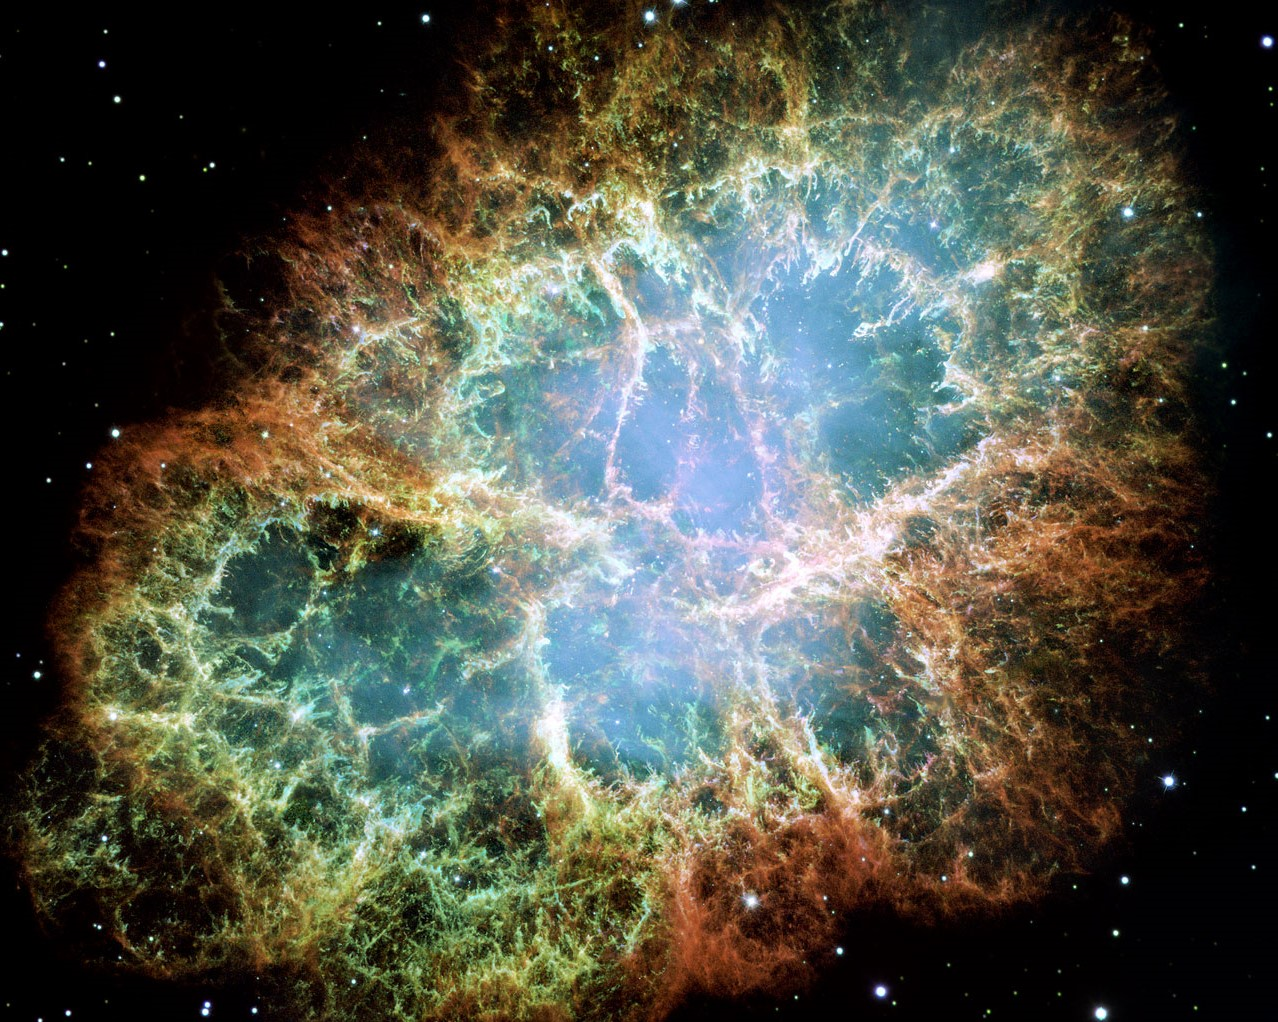
\includegraphics[width=\paperwidth, height =10cm]{../../Crab.jpg}}
    \end{figure}
\end{titlepage}

%%%%%%%%%%%%%%%%%%%%%%%
\tableofcontents

%%%%%%%%%%%%%%%%%%%%%%%%%%%%%%%%%%%%% Part 1
\part{Single Variable Analysis}

%%%%%%%%%%%%%%%%%%%%%% - P1.Chapter 1
%%%%%%%%%% Real Line %%%%%%%%%%
\chapter{Topology and Construction of the Real Line}\label{RealLineCons}
% use \chaptermark{}
% to alter or adjust the chapter heading in the running head


\section{Peano Arithmetic}

We begin by forming our number system from the ground up, starting wtih Giuseppe Peano's (1858-1932) axiomatized system for the natural numbers.

\begin{axiom}[Peano's Axioms]\index{Peano Arithmetic}
    Peano's system for the naturals consists of two central axioms: \begin{enumerate}
        \item Assume that there exists a set $\N$ and an element $0 \notin \N$. Define, notationally, $\tilde{\N} = \N\cup\{0\}$. Then, assume there exists an injective map $s:\tilde{\N}\rightarrow \N$ called the \Emph{successor function}
        \item \Emph{Mathematical Induction}: Whenever a subset $S \subseteq \tilde{\N}$ satisfies $0 \in S$, and if $k \in S$ then $s(k) \in S$, then this implies $S = \tilde{\N}$. Notationally we have $$(0 \in S \land (k \in S \implies s(k) \in S)) \implies S = \tilde{\N}$$
    \end{enumerate}
\end{axiom}

Given these axioms, we can define an addition operation on $\tilde{\N}$:
\begin{definition}\index{Binary Operation}
    We define the binary operation $+:\tilde{\N}\times\tilde{\N}\rightarrow\tilde{\N}$ inductively for $x,y \in \tilde{\N}$ by stating \begin{enumerate}
        \item $x + 0 = x$ 
        \item $x + s(y) = s(x+y)$ 
    \end{enumerate}
\end{definition}

The definition is performed inductively, or recursively. Fix $x \in \tilde{\N}$ and let $S = \{y \in \tilde{\N}:x+y\text{ is defined}\}$. By definition $0 \in S$. Further, if $y \in S$, $x+y$ is defined in $\tilde{\N}$, so $x+s(y) := s(x+y)$. Since $x+y \in \tilde{\N}$, by axiom 1 of Peano's arithmetic $s(x+y) \in \N\subset \tilde{\N}$. Thus, $s(x+y)$ is defined so $s(y) \in S$. Hence by mathematical induction $S = \tilde{\N}$ so $+$ is a well defined binary operation for all $x,y \in \tilde{\N}$.

We can similarly define multiplication:

\begin{definition}\index{Successor}
    We define the binary operation $\cdot:\tilde{\N}\times\tilde{\N}\rightarrow\tilde{\N}$ inductively for $x,y \in \tilde{\N}$ by stating \begin{enumerate}
        \item $x \cdot 0 = 0$ 
        \item $x \cdot s(y) = x\cdot y + x$ 
    \end{enumerate}
\end{definition}

This defines $x\cdot y$ inductively as in the case of $+$. Now, we define our unit:
\begin{definition}
    We define $1 \in \N$ by $1 := s(0)$.
\end{definition}

Now we can derive many of the standard properties of the naturals.

\begin{proposition}\label{prop:1.1.1}
    For all $x \in \tilde{\N}$, $x+1 = s(x)$.
\end{proposition}
\begin{proof}
    Let $x \in \tilde{\N}$. Then $x + 1 = x+s(0)$, but then by our inductive definition for $+$, $x+s(0) = s(x+0)$, and $x+0 = x$ by definition, so $$x+1 = s(x)$$
\end{proof}

\begin{proposition}\label{prop:1.1.2}
    For all $x \in \tilde{\N}$, $0+x = x$.
\end{proposition}
\begin{proof}
    We proceed by induction on $x \in \tilde{\N}$. If $x = 0$, then $0 + 0 = 0 = x$, by definition. Suppose inductively that we have $x \in \tilde{\N}$ such that $0+x=x$. Then $0+s(x) = s(0+x)$. But, $0+x = x$ by the induction hypothesis, so $0+s(x) = s(x)$ and our result holds for $s(x)$. Thus, by mathematical induction we conclude that $0+x = x$ for all $x \in \tilde{\N}$.
\end{proof}

\begin{proposition}\label{prop:1.1.3}
    For all $x,y \in \tilde{\N}$, $s(y) + x = s(y+x)$.
\end{proposition}
\begin{proof}
    Let $y \in \tilde{\N}$, and we proceed by induction on $x \in \tilde{\N}$. If $x = 0$ then $s(y)+0 = s(y)$, and $s(y+0) = s(y)$, so the base case holds. Now, suppose the proposition holds for some $x \in \tilde{\N}$. Then $s(y) + s(x) = s(s(y) + x)$ by definition, and by the induction hypothesis $s(y) + x = s(y+x) = y+s(x)$ by definition. Thus, $s(y)+s(x) = s(y+s(x)$, as desired. Thus, by mathematical induction we conclude taht $s(y) + x = s(y+x)$ for all $x,y \in \tilde{\N}$.
\end{proof}

\begin{proposition}\label{prop:1.1.4}
    For all $x, y \in \tilde{\N}$, $x+y = y+x$ (Commutative Law).
\end{proposition}
\begin{proof}
    Fix $x \in \tilde{\N}$, and we proceed by induction on $y \in \tilde{\N}$. If $y = 0$ then $x+0 = x$ by definition, and $0+x = x$ by Proposition \ref{prop:1.1.2}, so the base case holds. Now, suppose the proposition holds for some $y \in \tilde{\N}$. Then $x+s(y) = s(x+y)$ by definition, and by Proposition \ref{prop:1.1.3} we have $s(y)+x = s(y+x)$. By the induction hypothesis $x+y = y+x$, so $s(x+y) = s(y+x)$, and it follows that $s(y)+x = x+s(y)$. Hence, as $x$ was arbitrary, we have by mathematical induction that $x+y = y+x$ for all $x,y \in \tilde{\N}$.
\end{proof}

\begin{proposition}\label{prop:1.1.5}
    For all $x,y,z \in \tilde{\N}$, $x+(y+z) = (x+y)+z$ (Associative Law).
\end{proposition}
\begin{proof}
    Fix $x,y \in \tilde{\N}$, and proceed by mathematical induction on $z \in \tilde{\N}$. If $z = 0$, $x+(y+0) = x+y = (x+y)+0$, so the base case holds. Suppose the proposition holds for some $z \in \tilde{\N}$. Then it follows that \begin{align*}
        x+(y+s(z)) &= x + s(y+z) = s(x+(y+z)) \\
        &= s((x+y)+z) \tag{by Induction Hypothesis} \\
        &= (x+y)+s(z)
    \end{align*}
    as desired. Thus by the axiom of mathematical induction we have our result.
\end{proof}

\begin{proposition}\label{prop:1.1.6}
    For all $x \in \tilde{\N}$, $x\cdot 1 = x$.
\end{proposition}
\begin{proof}
    Fix$ x \in \tilde{\N}$. Then $x\cdot 1 = x\cdot s(0) := x\cdot 0 + x = 0 + x = x$, by Proposition \ref{prop:1.1.4}.
\end{proof}

\begin{proposition}\label{prop:1.1.7}
    For all $x \in \tilde{\N}$, $0\cdot x = 0$.
\end{proposition}
\begin{proof}
    We proceed by induction on $x \in \tilde{\N}$. If $x = 0$, $0\cdot 0 = 0$ by definition. If $0\cdot x = 0$ for some $x \in \tilde{\N}$, then $0 \cdot s(x) = 0\cdot x + 0 = 0$, so by mathematical induction we have our result.
\end{proof}

\begin{proposition}\label{prop:1.1.8}
    For all $x,y \in \tilde{\N}$, $s(x)\cdot y = x\cdot y + y$.
\end{proposition}
\begin{proof}
    Fix $x \in \tilde{\N}$, and proceed by induction on $y \in \tilde{\N}$. If $y = 0$, $s(x)\cdot 0 = 0 = x\cdot 0 + 0$. Suppose the result holds for some $y \in \tilde{\N}$. Then $s(x)\cdot s(y) = s(x)\cdot y + s(x)$ by definition, and $s(x)\cdot y = x\cdot y + y$ by the induction hypothesis. By Proposition \ref{prop:1.1.5}, $(x\cdot y+y)+s(x) = x\cdot y + (y+s(x)) = x\cdot y + s(y+x)$. By Proposition \ref{prop:1.1.4}, $x\cdot y + s(y+x) = x\cdot y + s(x+y) = x\cdot y + (x+s(y))$. Finally, by Proposition \ref{prop:1.1.5} again we have $x\cdot y + (x+s(y)) = (x\cdot y + x) + s(y) = x\cdot s(y)+s(y)$, as desired. The result follows by the principle of mathematical induction.
\end{proof}

\begin{proposition}\label{prop:1.1.9}
    For all $x,y \in \tilde{\N}$, $x\cdot y = y\cdot x$.
\end{proposition}
\begin{proof}
    Fix $x \in \tilde{\N}$, and proceed by mathematical induction on $y \in \tilde{\N}$. If $y = 0$, $x \cdot 0 = 0 = 0\cdot x$ by Proposition \ref{prop:1.1.7}, so the base case holds. Suppose it holds for some $y \in \tilde{\N}$. Then $x\cdot s(y) = x\cdot y + x = y\cdot x + x$ by the induction hypothesis, and by Proposition \ref{prop:1.1.8}, $y\cdot x + x = s(y)\cdot x$. Thus by mathematical induction we have commutivity of multiplication.
\end{proof}

\begin{proposition}\label{prop:1.1.10}
    For all $x,y,z \in \tilde{\N}$, $(x+y)\cdot z = x\cdot z + y \cdot z$ (Distributivity).
\end{proposition}
\begin{proof}
    Fix $x,z \in  \tilde{\N}$ and proceed by induction on $y \in \tilde{\N}$. If $y = 0$, $(x+0)\cdot z = x\cdot z = x\cdot z + 0\cdot z$ by Proposition \ref{prop:1.1.7}. Suppose it holds for some $y \in \tilde{\N}$. Then $(x+s(y))\cdot z = s(x+y)\cdot z = (x+y)\cdot z + z$ by Proposition \ref{prop:1.1.8}. By the induction hypothesis, associativity, and the same proposition again we have $$(x+y)\cdot z + z = (x\cdot z + y \cdot z) + z = x\cdot z + (y\cdot z + z) = x\cdot z + s(y)\cdot z$$
    as desired. Thus we have distributivity of multiplication by mathematical induction.
\end{proof}

\begin{proposition}\label{prop:1.1.11}
    For all $x,y,z \in \tilde{\N}$, if $x+z = y+z$, then $x = y$.
\end{proposition}
\begin{proof}
    Let $x,y \in \tilde{\N}$, and we proceed by induction on $z \in \tilde{\N}$. If $z = 0$, $x+0 = y+0$ implies $x = y$, so the base case holds. If it holds for some $z \in \tilde{\N}$, then $x+s(z) = y+s(z)$ implies $s(x+z) = s(y+z)$. But $s$ is an inductive function, so $x +z = y+z$ which implies $x = y$ by the induction hypothesis, and by mathematical induction we have our result.
\end{proof}

\begin{proposition}\label{prop:1.1.12}
    If $x \cdot z = y \cdot z$ and $z \neq 0$, then $x =y$.
\end{proposition}
\begin{proof}
    Suppose $x,y,z \in \tilde{\N}$ such that $x\cdot z = y\cdot z$. We argue by contrapositive and suppose $x \neq y$. Then by Trichotomy (to be shown) $x < y$ or $y < x$. Without loss of generality suppose $x < y$. Then $y = x+u$ for some $u \in \N$. Then $y\cdot z = x\cdot z + u\cdot z$, and so $u\cdot z = 0$ by the cancellation property. If $z \neq 0$, $z = s(w), w \in \tilde{\N}$, so $0 = u\cdot z = u\cdot w + u$. As $u \in \N$ this implies $u\cdot w < 0$, but $0 \leq k$ for all $k \in \tilde{\N}$ which contradicts trichotomy.
\end{proof}

As noted in the previous proof we used properties of the standard order relation on the naturals which we shall now define and prove.

\begin{definition}
    If $x,y \in \tilde{\N}$ we say \begin{enumerate}
        \item $x < y$ if $y = x+u$ for some $u \in \N$
        \item $x \leq y$ if $y = x+v$ for some $v \in \tilde{\N}$
    \end{enumerate}
\end{definition}

We could also say $x \leq y$ if and only if $y \in Rx = \{x+v:v \in \tilde{\N}\}$.  We define $y > x \iff x < y$ and $y \geq x \iff x \leq y$ for all $x,y \in \tilde{\N}$.

\begin{proposition}\label{prop:1.1.13}
    For $x,y \in \tilde{\N}$, if $x \leq y$ and $y \leq x$, then $x =y$.
\end{proposition}
\begin{proof}
    As $y = x+v, v \in \tilde{\N}$, and $x = y+u$ for $u \in \tilde{\N}$ by definition, $x = x+v+u$, so by the cancellation property $v + u = 0$. Towards a contradiction suppose $v$ or $u$ is not $0$. Without loss of generality suppose $v \neq 0$, so $v \in \N$ and there exists $m \in \tilde{\N}$ such that $v = s(m)$. Then $0 = u+s(m) = s(u+m) \in \N$, which contradicts our axiom that $0 \notin \N$. Thus, $v = u = 0$, so $x = y$.
\end{proof}

\begin{proposition}[Trichotomy]\label{prop:1.1.14}
    If $x,y \in \tilde{\N}$, then one and only one of the following hold: $$x < y \text{ or } x = y \text{ or } x > y$$
\end{proposition}
\begin{proof}
    Let $x,y \in \tilde{\N}$. If $x < y$ then $y = x+u$ for some $u \in \N$. If $x =y$ then $u = 0$, but $u \in \N$ so $u \neq 0$, and $x \neq y$. If $x > y$ then $x = y+v,$ $v \in \N$, but by the proof of Proposition \ref{prop:1.1.13} this implies $u=v=0$ contradicting the fact $u,v \in \N$. By similar arguments $x =y \implies x \cancel{<} y, x \cancel{>} y$, and $x > y$ follows from the first case. Let $y \in \tilde{\N}$ and proceed by induction on $x \in \tilde{\N}$. If $x = 0$, $y = y+0$ so $y \geq x$. If $y = 0$, $x = y$, and if $y \neq 0$, $y \in \N$ so $y > x$. Suppose the claim holds for some $x \in \tilde{\N}$. If $x < y$, then $s(x) \leq y$. Then either $s(x) = y$ or $s(x) + u = y$ for some $u \neq 0$, so $u \in \N$ and $s(x) < y$. If $x = y$, $s(x) = x+1 = y+1$, so $y < s(x)$. A similar argument holds if $y < x$, since $y < s(x)$, completing the induction.
\end{proof}

We now define the partial function of subtraction on $\tilde{\N}$:

\begin{definition}
    If $x,y \in \tilde{\N}$ with $x \leq y$, then we define $z := y-x \iff y = x+z$, where $z \in \tilde{\N}$.
\end{definition}
Notice $y-x$ is well defined by the cancellation property of addition.

\begin{proposition}\label{prop:1.1.17}
    If $x,y,u \in \tilde{\N}$, with $x \leq y$, then $(y-x)u = yu-xu$.
\end{proposition}
\begin{proof}
    Let $x,y \in \tilde{\N}$ with $x \leq y$ and let $u \in \tilde{\N}$. Then there exists $w \in \tilde{\N}$ such that $y = x+w$, so $yu = xu+wu$ by distributivity, Then by definition $yu - xy = wu = (y-x)u$.
\end{proof}

Next we move on to a central property of the natural numbers which is equivalent to the axiom of mathematical induction:

\begin{theorem}[Well-Ordering Property of $\tilde{\N}$]\label{namthm:wellOrder}\index{Well-Ordering Property}
    If $T \subseteq \tilde{\N}$ is non-empty, then $T$ has a smallest element.
\end{theorem}
\begin{proof}
    We proceed by contrapositive. Suppose $T \subseteq \tilde{\N}$ and $T$ has no smallest element. Then $0 \notin T$, since for all $x \in \tilde{\N}$, $0 \leq x$, as either $x = 0$ or $x \in \N$ so $x = x+0$ and $x > 0$. Let $S = \{x \in \tilde{\N}:x < y,\forall y \in T\}$, so $0 \in S$. Inductively suppose $x \in S$. If $s(x) \in S$, we're done, so suppose $s(x) \geq y$ for some $y \in T$. But $x < y$, so $y = x+s(w)$, for some $w \in \tilde{\N}$, and $y = s(x)+w$. Thus $s(x) \leq y$, so by Proposition \ref{prop:1.1.13}, $s(x) = y \in T$. But $s(x) \leq t$ for all $t \in T$, so $s(x)$ is a minimal element of $T$, contradicting the hypothesis. Thus $s(x) \in S$, so by mathematical induction $S = \tilde{\N}$. Then as $T \subseteq \tilde{\N}\backslash S$, $T = \emptyset$ as desired.
\end{proof}

In the next section we perform an arithmetic closure of the naturals to obtain the rational field, $\Q$.


\section{Construction of The Rational Field}

First we need the notion of an equivalence relation for our constructions:

\begin{definition}[Equivalence Relation]\index{Equivalence relation}
    An equivalence relation on a set $S$ is a subset $E \subseteq S\times S$ such that \begin{enumerate}
        \item For all $x \in S$, $xEx$ (reflexivity) 
        \item For all $x,y \in S$, if $xEy$ then $yEx$ (symmetry) 
        \item For all $x,y,z \in S$, if $xEy$ and $yEz$, then $xEz$ (transitivity)
    \end{enumerate}
\end{definition}

An important property of equivalence relations is there relation to partitions of a set: in particular, we have a bijection between partitions of a set and equivalence relations.

\begin{definition}\Alsoindex{Equivalence relation}{Equivalence class}
    For an equivalence relation $\sim$ on a set $S$, and $x \in S$, the \Emph{equivalence class} for $x$ is defined by \begin{equation*}
        [x]_{\sim} := \{y \in S: x \sim y\}
    \end{equation*}
\end{definition}

Note that $[y]_{\sim} = [x]_{\sim}$ if and only if $x \sim y$. Further, the equivalence classes for $\sim $ form a partition on $S$. That is $S = \cup_{x \in S}[x]_{\sim}$, and if $[y]_{\sim} \neq [x]_{\sim},$ $[y]_{\sim}\cap[x]_{\sim} = \emptyset$.

\begin{definition}
    Define $\sim$ on $\tilde{\N}\times \tilde{\N}$ by $(a,b) \sim(x,y)$ if and only if $a+y = x+b$.
\end{definition}
We consider $(a,b)$ to be $a-b$. We note that this defines an equivalence relation, we the proof left to the reader.

\begin{definition}\index{Integers}
    We define the \Emph{Integers}, $\Z$, to be the set \begin{equation*}
        \Z := \{[(x,a)]_{\sim} \in \mathcal{P}(\tilde{\N}\times\tilde{\N}): x,a \in \tilde{\N}\} = \tilde{\N}\times\tilde{\N}/\sim
    \end{equation*}
    and we have the natural injection \begin{align*}
        \iota:\tilde{\N}&\rightarrow \Z \\
        x&\mapsto [(x,0)]
    \end{align*}
\end{definition}

We can define operations of addition and multiplication on $\Z$ inherited from $\tilde{\N}$.

\begin{definition}
    For $[(x,a)],[(y,b)] \in \Z$, we define \begin{align*}
        [(x,a)]+[(y,b)] &= [(x+y,a+b)] \\
        [(x,a)]\cdot[(y,b)] &= [(xy + ab, xb + ay)]
    \end{align*}
\end{definition}
To show these definitions are well defined we must show that the operation is independent of the choice of representative of each equivalence class. This is a routine check left to the reader.

\begin{definition}
    We define $0 = [(0,0)]$ and $-1 = [(0,1)]$ in $\Z$, and if $m = [(x,a)]$, we define $-m := [(a,x)]$.
\end{definition}

\begin{proposition}
    For all $m \in \Z$, $m \cdot (-1) = -m$.
\end{proposition}
The proof is a quick calculation: \begin{equation*}
    m\cdot (-1) = [(x,a)][(0,1)] = [(x\cdot 0+a,x+a\cdot 0)] = [(a,x)] = -m
\end{equation*}

Similarly, we have all the properties we derived for $\tilde{\N}$ for the operations on $\Z$, such as $m\cdot 0 = 0$, $m(n+k) = mn+mk$, $m+n=m+k \implies n =k$, and $m\cdot n= k\cdot n\implies m=k$ if $n \neq 0$. Now we have closed the $\tilde{\N}$ under ring operations, obtaining the integral domain $\Z$.

Next we perform a similar construction to obtain our field - this process is known as constructing a fraction field for an integral domain.

\begin{definition}
    Define an equivalence relation $\sim$ on $\Z\times \Z\backslash\{0\}$ by $(x/a)\sim(y/b)$ if and only if $xb = ya$, for $(x/a),(y/b) \in \Z\times \Z\backslash\{0\}$.
\end{definition}

It is routine to show that this is indeed an equivalence relation on the set. Next, we can define addition and multiplication operations:

\begin{definition}\index{Rationals}
    We define the rationals to be \begin{equation*}
        \Q = \Z\times \Z\backslash\{0\}/\sim
    \end{equation*}
    For $[m/n],[a/b] \in \Q$, we define $$[m/n] + [a/b] = [(mb+an)/(nb)]$$ and $$[m/n]\cdot[a/b] = [(ma)/(nb)]$$
\end{definition}

It is a routine varification that these operations are well-defined and independent of the representative. If $x = [(a/b)] \in \Q$, and $x \neq 0$ so $a \neq 0$, then we can define $$x^{-1} = \frac{1}{x} := [(b/a)] \in \Q$$ We also define $0 := [0/1], 1 := [1/1],$ and $-1 := [-1/1]$. So far we have the chain $$\tilde{\N}\hookrightarrow \Z := \tilde{\N}\times \tilde{\N}/\sim \hookrightarrow \Z\times (\Z\backslash\{0\})/\sim$$

\section{Divisibility}

We now go over some fundamental theorems of number theory involving divisibility.

\begin{definition}
    We say $x \in \N$ is \Emph{composite} if $a,b \in \N$ such that $x = ab$ and $a,b \neq 1$. If $x$ is not composite, and $x > 1$, then $x$ is said to be \Emph{prime}. That is, $x$ is prime if and only if $x = ab$ implies $a = 1$ or $b =1$.
\end{definition}

\begin{definition}\index{Divisor}
    If $x = ab$, $x,a,b \in \N$, then we say $a$ \Emph{divides} $x$, or $a$ is a \Emph{divisor} of $x$, and we write $a\;\vert\;x$.
\end{definition}

\begin{definition}
    Given $x \in \N$, define the collection of non-trivial divisors as $$D_x := \{a \in \N\backslash\{1\}:a\;\vert\;x\} \subseteq \N$$
\end{definition}

Note that if $a \;\vert\;x$, then $a \leq x$. As $D_x \subseteq \N$, and $x \in D_x$ so it is non-empty, $D_x$ has a smallest element $p_1 \in D_x$. Then $x = p_1x_1$ for some $x_1 \in \N$. Then $p_1$ is prime since if note it can be written as $p_1 = ab$ for $1 < a < p_1$, and then $a\;\vert\;x$ with $a < p_1$, contradicting its minimality. If $x_1 > 1$, then we can obtain $x_1 = p_2x_2$, for $p_2$ prime and $p_2 \geq p_1$. Repeating in this fashion, since $x$ is finite there must exist $N \in \N$ such that $x_N = 1$ and $x_{N-1} = p_N\cdot 1$. Then $x = p_1\cdot ...\cdot p_N$. This is the existence portion of the following result.

\begin{theorem}[Fundamental Theorem of Arithmetic]\index{Fundamental Theorem of Arithmetic}
    Every natural number $x > 1$ has a unique factorization, up to reordering, into a product of prime numbers.
\end{theorem}
\begin{proof}
    If $x = p_1...p_N = q_1...q_M$, then for each $1 \leq i\leq N$, $p_i\;\vert\;q_j$ for some $1 \leq j \leq M$. But, $p_i$ and $q_j$ are prime, so $p_i = q_j$, and after reordering $p_1 ...p_N = p_1...p_Nq_{N=1}...q_M$. By cancellation $q_{N+1}...q_M = 1$. Thus, $N = M$ and the terms are equal up to reordering.
\end{proof}

\begin{definition}
    We say $x,y \in \N$ are \Emph{coprime} if $x$ and $y$ have no common prime factors.
\end{definition}

\begin{proposition}
    If $x,y \in \N$ are coprime, then there exists $m,n \in \Z$ such that $$xm+ny = 1$$
\end{proposition}

\section{Reals in terms of Cauchy Sequences}

To construct the reals we use the standard notion of a completion of metric spaces using equivalence classes of Cauchy sequences. But first we must define what a sequence is, and what it means for one to be Cauchy.

\begin{definition}
    We define the \Emph{absolute value function} by $$|x| = \left\{\begin{array}{cc} x & \text{if }x \geq 0 \\ -x & \text{if } x < 0\end{array}\right.$$
\end{definition}

It is a standard proof by cases, that the absolute value function defines a norm on $\Q$.

\begin{definition}\index{Sequence}
    A sequence is a function $a:\N\rightarrow \Q$, denoted $a(j) = a_j$ and $(a_j)_{j=1}^{\infty}$.
\end{definition}

\begin{definition}\index{Convergence}
    We say a sequence $(a_j)$ converges to a number $a \in \Q$, and write $a_j\rightarrow a$, if for every $n \in \N$, there exists an index $K(n) \in \N$ such that if $j\geq K(n)$, then $|a_j - a| < \frac{1}{n}$.
\end{definition}

\begin{definition}\index{Cauchy}
    A sequence $(a_j)$ is said to be \Emph{Cauchy} if for all $n \in \N$, there exists $K(n) \in \N$ such that if $j,k \geq K(n)$, then $$|a_j - a_k| < \frac{1}{n}$$
\end{definition}

\begin{proposition}
    If $a_j\rightarrow a$, then $(a_j)$ is Cauchy.
\end{proposition}
\begin{proof}
    Since $a_j \rightarrow a$, for $n \in \N$ there exists $K(2n) \in \N$ such that if $j \geq K(2n)$, $|a_j - a| < \frac{1}{2n}$. Thus, if $k,j \geq K(2n)$, then $$|a_j - a_k| \leq |a_j - a| + |a - a_k| < \varepsilon$$ as desired.
\end{proof}

\begin{proposition}
    If $(a_j)$ is Cauchy then $(a_j)$ is bounded.
\end{proposition}
\begin{proof}
    Suppose $(a_j)$ is Cauchy. Then there exists $K(1) \in \N$ such that for $k,j\geq K(1)$, $|a_k - a_j| < 1$. Then for all $j \geq K(1)$, $|a_j| < 1 + |a_{K(1)}|$. Letting $M = \max\{|a_1|,...,|a_{K(1)-1}|, 1+|a_{K(1)}|\}$, we have that $a_n \leq M$ or all $n \in \N$, so the sequence is bounded.
\end{proof}

We now have some standard results about convergence of sequences:

\begin{proposition}\label{prop:1.5.1}
    If $a_j\rightarrow a$ and $b_j\rightarrow b$, then $$a_j+b_j\rightarrow a+b,\;\text{ and }\;a_jb_j\rightarrow ab$$ If $b \neq 0$, and $b_j \neq 0$ for all $j$, then $$a_j/b_j\rightarrow a/b$$
\end{proposition}

More generally we have 
\begin{definition}
    If $(a_j),(b_j)$ are Cauchy sequences, then $(a_j+b_j)$ is Cauchy, $(a_jb_j)$ is cauchy, and if there exists $n \in \N$ such that $|b_j| > \frac{1}{n}$ for all $j$, then $(a_j/b_j)$ is Cauchy.
\end{definition}

Although for general metric spaces we have the inclusion $$\left\{\begin{array}{cc} Convergent \\ Sequences\end{array}\right\} \subseteq \left\{\begin{array}{cc} Cauchy \\ Sequences \end{array}\right\}$$
the other inclusion is not in general true.

\begin{example}
    Let $a_j = \sum_{l=0}^j\frac{1}{l!}$, in $(\Q, d)$, $d(x,y) = |x-y|$. $a_j$ is a Cauchy sequence, as $|a_j - a_k| = \left|\sum_{l=k+1}^j\frac{1}{l!}\right| = \sum_{l=k+1}^j\frac{1}{l!}\rightarrow 0$. For $l\geq 2$ we have $\frac{1/(l+1)!}{1/l!} = \frac{1}{l} \leq \frac{1}{2}$. Then $\frac{1}{(2+j)!} \leq \frac{1}{2^j}\frac{1}{2}$. Then for $j > k \geq 2$, $$\sum_{l=k+1}^j\frac{1}{l!} = \sum_{l=k-2}^{j-2}\frac{1}{(l+2)!} \leq \sum_{l=k-2}^{l-2}\frac{1}{2^l}\frac{1}{2} < \frac{1}{2}\frac{1}{1-1/2} = 1$$ Thus, $a_j$ is a bounded increasing sequence and hence Cauchy. Now observe \begin{align*}
        a_{n+j}-a_n &= \frac{1}{(n+1)!} + ... + \frac{1}{(n+j)!} \\
        &\leq \frac{1}{n!}\left(\frac{1}{n+1}+ \frac{1}{(n+1)^2} + ... + \frac{1}{(n+1)^j}\right) \\
        &< \frac{1}{n!}\sum_{k=0}^{j-1}\frac{1}{(n+1)^{k+1}} \\
        &= \frac{1}{(n+1)!}\frac{1-\frac{1}{(n+1)^{j-1}}}{1-\frac{1}{n+1}} < \frac{1}{n!n}
    \end{align*}
    So if we fix $N \in \N$, $N+j > N+k \geq N$, then $a_{N+j} - a_{N+k} < \frac{1}{N!N} < \frac{1}{N}$. Hence $a_j$ is Cauchy. Since it is Cauchy, in the complete metric space $\R$ it is convergent, so let $a = \lim a_j$, so we observe $a = \sum_{l=0}^{\infty}\frac{1}{l!} = e$. But $e \notin \Q$, so this limit cannot be in the rationals and hence the rationals is not complete. 
\end{example}

The following is a very important series known as the \Emph{geometric series}:

\begin{proposition}
    If $a \in \Q$, with $|a| < 1$, then $\sum_{j=0}^{\infty}a^j = \frac{1}{1-a}$.
\end{proposition}

\begin{proposition}
    If $|a| < 1$, then $|a|^n\rightarrow 0$.
\end{proposition}
\begin{proof}
    If $a = 0$, then $|a|^n = 0$ for all $n$, so the result holds. Hence, suppose $a \neq 0$. Then $|a|^{j+1} < |a|^j$, so $|a|^n$ is a bounded decreasing sequence, and hence converges in $\R$. Hence $\lim\limits_{n\rightarrow \infty}|a|^n = k$ for some $k \in \R$. Then $k = \lim\limits_{n\rightarrow \infty}|a|^n = \lim\limits_{n\rightarrow \infty}|a|^{n+1} = |a|k$. But $|a| \neq 1$, so $k = 0$. Thus, $|a|^n\rightarrow 0$, as desired.
\end{proof}


\begin{proposition}[Bolzano-Weierstrass (Cauchy)]\index{Bolzano-Weierstrass}
    If $(a_j)$ is a bounded sequence, then there exists a Cauchy subsequence.
\end{proposition}
\begin{proof}
    Since $(a_j)$ is bounded, there exists $M > 0$ such that $|a_j| \leq M$ for all $j$. In particular, $a_j \in I_0 = [-M,M]$ for all $j$. Then either $[-M,0]$ or $[0,M]$ contains an infinite number of $a_j$. Let $I_1$ be the one with such. Inductively, suppose there exists $k \in \tilde{\N}$ such that an infinite number of $a_j$ are in $I_k$, for all $0 \leq l \leq k-1$ $I_{l+1}\subseteq I_l$, and $\ell(I_l) = \frac{2M}{2^l}$. Then, we have a sequence $I_j$ of closed intervals containing infinitely many terms of $a_j$. Let $b_1 = a_1$, and let $b_k = a_{j(k)}$, where $j(k) = \min\left\{m \in \N: a_m \in I_k, m > j(k-1)\right\}$, which exists and is well defined by the construction of $I_k$ and the well-ordering of $\N$. Then $b_k = a_j(k)$ is a subsequence of $j$, as $j(k) < j(k+1)$ for all $k$. Now, fix $n \in \N$. As $2^{-j}\rightarrow 0$, there exists $K(2Mn) \in \N$ such that for $j \geq K(2Mn)$, $\frac{1}{2^j} < \frac{1}{2Mn}$. Then, for $k,l \geq K(2Mn)$, $b_k,b_l \in I_{K(2Mn)}$, so $$|b_k - b_l| \leq \ell(I_{K(2Mn)}) = \frac{2M}{2^{K(2Mn)}} < \frac{2M}{2Mn} = \frac{1}{n}$$ Thus $b_j$ is Cauchy.
\end{proof}

\begin{corollary}
    Each bounded Monotone sequence is Cauchy.
\end{corollary}
\begin{proof}
    Let $(a_j)$ be a bounded monotone sequence. Then we have a Cauchy subsequence $(a_{j_n})$. Fix $n \in \N$. Then there exists $K(n) \in \N$ such that if $k,l \geq K(n)$, $|a_{j_k} - a_{j_l}| < \frac{1}{n}$. Let $K'(n) = j_{K(n)}$. Then for $k,l \geq K'(n)$, let $m \in \N$ such that $j_m \geq k,l$ and $m \geq K(n)$. Then as $a_j$ is an increasing (decreasing) sequence, so $$a_{j_{K(n)}} \leq a_k \leq a_l \leq a_{j_m}\;(\text{respectively }a_{j_{K(n)}} \geq a_k \geq a_l \geq a_{j_m})$$ Then $0 \leq a_l - a_k \leq a_{j_m} - a_{j_{K(n)}}$, so $|a_l - a_k| < \frac{1}{n}$, and similarly for a decreasing sequence. Hence $a_j$ is Cauchy.
\end{proof}

We now begine defining the reals using equivalence relations on our Cauchy sequences:

\begin{definition}
    Let $\mathcal{S} = \{(a_j) \subseteq \Q:(a_j) \text{ is Cauchy}\}$. Define an equivalence relation $\sim$ on $\mathcal{S}$ by $$(a_j)\sim (b_j) \iff a_j-b_j\rightarrow 0$$
\end{definition}

It is a routine check that $\sim$ is an equivalence relation on $\mathcal{S}$. 

\begin{definition}\index{Reals}
    We define $\R := \mathcal{S}/\sim$, so $x \in \R$ if and only if $x = [(a_j)]$ for some Cauchy sequence $(a_j)$ in $\Q$.
\end{definition}

\begin{definition}
    If $x = [(a_j)], y = [(b_j)] \in \R$, we define $$x+y := [(a_j+b_j)]\;\;xy := [(a_jb_j)]$$ and $-x := [(-a_j)]$.
\end{definition}

As with the notion of an equivalence relation, it is a routine check using the boundedness of Cauchy sequences to prove that these operations are well defined. We can then define a natural injection $\Q\hookrightarrow \R$ by $a\mapsto [(a,a,a,...)]$. In particular, $0:= [(0,0,0,...)]$ in $\R$. 

Now, note that if $x = [(a_j)], y = [(b_j)] \in \R$, then $x \neq y$ if and only if $a_j-b_j$ does not converge to $0$, so there exists $n \in \N$ such that for all $j \in \N$, there exists $k \geq j$ such that $$|a_k - b_k| \geq \frac{1}{n}$$ Specializing to the case of $y = 0=[(0,0,0,...)]$, as $(a_j)$ is Cauchy, there exists $K(2n) \in \N$ such that $k,l \geq K(2n)$, $|a_k - a_l| < \frac{1}{2n}$, so in particular $|a_j| \geq |a_k| - |a_j - a_k| > \frac{1}{2n}$ for all $j \geq K(2n)$. It follows that either $a_j > \frac{1}{2n} > 0$ for all $j \geq K(2n)$, or $a_j < \frac{-1}{2n} < 0$ for all $j \geq K(2n)$.

Thus, if $x \neq 0$, then $x = [(a_j)] = [(\alpha_j)]$ such that there exists $n \in \N$ such that either $\alpha_j \geq \frac{1}{2n}$ for all $j$, or $\alpha_j \leq \frac{-1}{2n}$ for all $j$. Then we can define $x^{-1} = \frac{1}{x} := [(\alpha_j^{-1})]$.

\begin{definition}
    We define the following subsets of $\R$: \begin{align*}
        \R^+ &= \{x = [(a_j)]: \exists n,K \in \N;a_j\geq \frac{1}{2n},\forall j \geq K\} \\
        \R^- &= \{x = [(a_j)]: \exists n,K \in \N; a_j \leq \frac{-1}{2n},\forall j\geq K\}
    \end{align*}
\end{definition}
We have shown that if $x \neq 0$ then either $x \in \R^+$ or $x \in \R^-$. Thus $$\R = \R^+ \sqcup \{0\}\sqcup \R^-$$

\begin{proposition}
    For $x \in \R$, $x \in \R^+$ if and only if $-x \in \R^-$, and $x \in \R^-$ if and only if $-x \in \R^+$.
\end{proposition}

\begin{definition}
    We define a total order $<$ on $\R$ by $$x < y \iff y-x \in \R^+ \iff x = [(a_j)],y=[b_j)],\exists n,K \in \N;b_j-a_j \geq \frac{1}{2n}\forall j \geq K$$
\end{definition}

We have a few standard results about the order relation on $\R$: 

\begin{proposition}\label{prop:1.6.4}
    Let $x_1,x_2,y_1,y_2 \in \R$. Then \begin{itemize}
        \item $x_1 < y_1, x_2 < y_2 \implies x_1+x_2 < y_1 + y_2$
        \item $x_1 < y_1 \implies -y_1 < -x_1$
        \item $0 < x_1 < y_1$, $c > 0$, then $0 < cx < cy$
        \item $0 < x < y \iff 0 < \frac{1}{y} < \frac{1}{x}$
    \end{itemize}
\end{proposition}

Note that in $\N$ we have well-ordering, but under the standard orders on $\Q$ and $\R$ this property does not hold.

\begin{definition}\index{Bounds}
    For $S \subseteq \R$, we say $x$ is an \Emph{upper bound} of $S$ if $s \in S$ implies $s \leq x$. Dually, we say $y$ is a \Emph{lower bound} for $S$ is $s \in S$ implies $s \geq y$.
\end{definition}

\begin{definition}
    For $S \subseteq \R$, the \Emph{least upper bound}, denoted $\sup S$, is an upper bound for $S$ such that if $y$ is any other upper bound for $S$ then $\sup S \leq y$. Dually, the \Emph{greatest lower bound}, denoted $\inf S$, is a lower bound for $S$ such that if $y$ is any other lower bound for $S$, then $y \leq \inf S$.
\end{definition}

\begin{theorem}[Completeness of $\R$]\index{Completeness}
    If $(x_j)$ is a Cauchy sequence of real numbers, then there exists $x = [(a_j)] \in \R$ such that $x_j \rightarrow x$, of $x_j \sim a_j$, extending the equivalence relation to $\R$.
\end{theorem}


\begin{proposition}\label{prop:1.6.12}
    If $S$ is a non-empty subset of $\R$ that has an upper bound, then there exists $x \in \R$ such that $x = \sup S$.
\end{proposition}
\begin{proof}
    By hypothesis, there exists $x_0 \in \R$ such that for all $s \in S$, $s \leq x_0$. As $S$ is non-empty, there exists $s_0 \in S$. Define an interval $I_0 = [s_0,x_0]$, and divide it into $2$ subintervals, $I_0^l,I_0^r$. If $I_0^r\cap S \neq \emptyset$ let $I_1^* = I_0^r$, and otherwise let $I_1^* = I_0^l$. In either case $I_1 = [s_1,x_1]$ is such that $x_1$ is an upper bound of $S$, and where we choose $s_1 \in I_1^*$ such that $s_1 \in S$. Further, $s_0 \leq s_1 \leq x_1 \leq x_0$, and letting $x_0 - s_0 = L$, $\ell(I_1) \leq \frac{L}{2}$. Proceeding inductively we find sequences $s_0\leq s_1\leq s_2 \leq ...$ in $S$ and $x_0 \geq x_1 \geq x_2 \geq ...$, with $I_j = [s_j,x_j]$, $\ell(I_j) \leq \frac{L}{2^j}$, with $x_j \geq s$ for all $s \in S$, and all $j \in \tilde{\N}$. Note $x_j$ is a decreasing bounded sequence, so it converges to some $x \in \R$, as $\R$ is complete. As $x_j \geq s$ for all $s \in S$, $x \geq s$ so $x$ is an upper bound. Further, if $\varepsilon > 0$, there exists $K \in \N$ such that for all $j \geq K$, $\frac{1}{2^j} < \frac{\varepsilon}{L}$, so $0 \leq x_j - s_j < \frac{L}{2^j} < \varepsilon$ for all $j \geq K$. Then $x-\varepsilon < s_j$ for all $j \geq K$. Thus, $x-\varepsilon$ is not an upper bound of $S$, and hence $x$ must be the least upper bound.
\end{proof}


\section{Metric Properties of the Reals}

First we extend our definition of sequences to the reals:

\begin{definition}\index{Convergence}
    A sequence $(p_j)$ in $\R$ converges to a point $p \in \R$ if and only if for every $\varepsilon > 0$ there exists $N \in \N$ such that if $j \geq N$, then $|p_j - p| < \varepsilon$.
\end{definition}

Using sequences we can define notions of our topology, such as closed and open sets, and limit points:

\begin{definition}\index{Closed}
    $S \subseteq \R$ is said to be \Emph{closed} if and only if whenever $(p_j) \subseteq S$ is a sequence in $S$ which converges to a point $p \in \R$, then $p \in S$.
\end{definition}

\begin{definition}\index{Accumulation point}
    A point $p \in \R$ is said to be a \Emph{limit point} of $S$ if there exists $(p_j) \subseteq S$ such that $p_j$ converges to $p$, and $p_j \neq p$ for all $j \in \N$.
\end{definition}

Note that $S$ is closed if and only if $S$ contains all of its limit points.

\begin{definition}\index{Open}
    $U\subseteq \R$ is said to be \Emph{open} if and only if $U^c = \R\backslash U$ is closed.
\end{definition}

\begin{definition}\index{Closure}
    For $S \subseteq \R$, the \Emph{closure} of $S$, $\overline{S}$, is defined as $$\overline{S}:= S \cup S'$$ where $$S' = \{p \in \R: p \text{ is a limit point of } S\}$$
\end{definition}

\begin{proposition}
    For all $S \subseteq \R$, $\overline{\overline{S}} = \overline{S}$
\end{proposition}
\begin{proof}
    Let $(p_j) \subseteq \overline{S}$ which converges to some point $p \in \R$. Then for each $j$ we have $(b_{jk})$ in $S$ which converges to $p_j$. For each $j \in \N$, there exists $K(j) \in \N$ such that for $k \geq K(j)$, $|b_{jk} - p| < \frac{1}{j}$. Define $(c_j)$ by $c_j = b_{jK(j)}$. Fix $\varepsilon > 0$. Then there exists $N \in \N$ such that $j \geq N$ implies $|p_j - p| < \frac{\varepsilon}{2}$. By the Archimedian property there exists $n \in \N$ such that $\frac{1}{n} < \frac{\varepsilon}{2}$. Then for a $j \geq \max\{n,N\}$, \begin{align*}
        |c_j - p| \leq |c_j - p_j| + |p_j - p| < \frac{1}{n} + \frac{\varepsilon}{2} < \varepsilon
    \end{align*}
    Thus $(c_j) \subseteq S$ and $c_j\rightarrow p$, so $p \in \overline{S}$. Hence, $\overline{S}\supseteq \overline{\overline{S}}$, and by definition $\overline{S} \subseteq \overline{\overline{S}}$, so $\overline{S} = \overline{\overline{S}}$.
\end{proof}

\begin{theorem}\label{thm:1.9.1}
    Every Cauchy sequence in $\R$ has a limit point in $\R$.
\end{theorem}

Note if $(x_j) = ([(a_{jk})])$ is Cauchy in $\R$, then $(a_{jj})$ is Cauchy in $\Q$ with $a_{jj} - x_j \rightarrow 0$, so then $x_j$ converges to $[(a_{jj})]$.

\begin{proposition}[Density of the Rationals]
    For all $x \in \R$ and $\varepsilon > 0$, there exists $y \in \Q$ such that $|y-x| < \varepsilon$.
\end{proposition}
In particular, for all $a < b$ in $\R$, there exists $c \in \Q$ such that $a < c < b$. Indeed, for $x = [(a_j)]$, $a_j \rightarrow x$ so there exists $N \in \N$ such that $|a_N - x| < \varepsilon$ for any $\varepsilon > 0$.

\begin{definition}
    A subset $K \subseteq \R$ is \Emph{sequentially compact} if and only if for every \Emph{infinite sequence} $(p_j) \subseteq K$, there exists a subsequence which converges to a point in $K$.
\end{definition}

\begin{theorem}[Bolzano-Weierstrass Property]\index{Bolzano-Weierstrass}
    Every bounded sequence of real numbers has a convergent subsequence.
\end{theorem}


\begin{theorem}\label{thm:1.9.2}
    If $K \neq \emptyset$, $K \subseteq \R$, and $K$ is closed and bounded, then $K$ is sequentially compact.
\end{theorem}
\begin{proof}
    If $K \subseteq \R$, $K \neq \emptyset,$ is bounded and $(p_j) \subseteq K$, $(p_j)$ has a convergent subsequence $(p_{j_k})$ by Bolzano-Weierstrass, so $p_{j_k}\rightarrow p$ for some $p \in \R$. But $K$ is closed so $(p_{j_k}) \subseteq K$, so $p \in K$.
\end{proof}

Note that if $K \subseteq \R$ is compact, then $K$ is closed since all subsequences of a convergent sequence converge to the same point. Additionally, $K$ is bounded as otherwise we can construct $p_1 \in K$, $p_2 \in K$ such that $|p_2| > |p_1| + 1$, and for $p_k \in K$, choose $p_{k+1} \in K$ such that $|p_{k+1}| > |p_k| + 1$. Thus, for all $j,k \in \N$, $|p_j - p_k| > 1$, so $(p_j)$ has no convergent subsequence.

\begin{theorem}[Heine-Borel]\index{Heine-Borel}
    If $K \neq \emptyset, K \subseteq \R$, the following are equivalent: \begin{itemize}
        \item $K$ is sequentially compact
        \item $K$ is closed and bounded
    \end{itemize}
\end{theorem}

If $K$ is compact, $K \neq \emptyset$, in $\R$, then there exists $a,b \in K$ such that $$a = \min K := \inf K\;\text{ and }\;b = \max K := \sup K$$ which is to say $K$ contains its infimum and supremum.

\begin{definition}\index{Continuity}
    A function $f:S\rightarrow \R$, $\emptyset \neq S \subseteq \R$, is said to be \Emph{continuous} at a point $p \in S$ if whenever $(p_j) \subseteq S$ such that $p_j\rightarrow p$, then $f(p_j)\rightarrow f(p)$
\end{definition}

\begin{definition}\index{Isolated Point}
    A point $p \in S$ is said to be an \Emph{isolated point} of $S$ if there exists some $\varepsilon > 0$ such that $(p-\varepsilon,p+\varepsilon) \cap S = \{p\}$
\end{definition}
Every function is continuous at isolated points of its domain.

\begin{definition}
    If $f:S\rightarrow \R$ is continuous at every point $p \in S$, we say $f$ is \Emph{continuous} on $S$.
\end{definition}

\begin{proposition}\label{prop:1.9.4}
    If $K \subseteq \R$, $K \neq \emptyset$, is a compact subset of $\R$, and $f:K\rightarrow \R$ is continuous, then $f(K)$ is compact.
\end{proposition}
\begin{proof}
    Let $(q_k) \subseteq f(K)$. Then we have $(p_k) \subseteq K$ such that $f(p_k) = q_k$ for all $k$. Then as $K$ is sequentially compact there exists $p \in K$ and a subsequence $(p_{k_j}) \subseteq K$ such that $p_{k_j}\rightarrow p$. As $f$ is continuous we have $q_{k_j} = f(p_{k_j}) \rightarrow f(p)$, where $f(p) \in f(K)$. Thus $f(K)$ is sequentially compact as claimed.
\end{proof}

\begin{proposition}\label{prop:1.9.5}
    If $\emptyset \neq K \subseteq \R$ is sequentially compact and $f:K\rightarrow \R$ is continuous on $K$, then there exist $q,p \in K$ such that $$f(p) = \max_{K}f,\;\;f(q) = \min_Kf$$
\end{proposition}

\begin{theorem}[Intermediate Value Theorem]\index{IVT}
    If $f:[a,b]\rightarrow \R$ is continuous on $[a,b]$ and $f(a) < c < f(b)$ (or $f(a) > c > f(b)$), then there exists $x \in (a,b)$ such that $f(x) = c$.
\end{theorem}
\begin{proof}
    Let $S = \{y \in [a,b]: f(y) \leq c\}$. Without loss of generality suppose $f(a) < c < f(b)$ (if the other inequality holds, replace $f$ with $-f$). THen $a \in S$ and $b \notin S$. Further, if $(y_j) \in S$, $y_j\rightarrow y$, then by continuity $f(y_j)\rightarrow f(y)$ and as $f(y_j) \leq c$ for all $j$, $f(y) \leq c$. Thus $y \in S$, so $S$ is closed. As $S \subseteq [a,b]$, $S$ is bounded, so by Heine-Borel $S$ is compact. Let $x = \max S \in S$. Then $f(x) \leq c$. If $f(x) < c$, then for some $\varepsilon > 0$, $f(y) < c$ for all $y \in (x-\varepsilon,x+\varepsilon)$. Let $\varepsilon = c-f(x) > 0$. As $f$ is continuous, there exists $\delta > 0$ such that if $|x-y| < \delta$, $|f(x) - f(y)| < \frac{\varepsilon}{2}$. Then $c-f(y) = c-f(x) - (f(y) - f(x)) \geq |c-f(x)| - |f(y) - f(x)|$, which is greater than or equal to $\varepsilon/2$, so $f(y) < c$. Taking $y = x+\frac{\delta}{2}$, $f(y) \leq c$, so $y \in S$, but $y > x = \max S$ which is a contradiction. Thus, $f(x) \cancel{<} c$, so $f(x) = c$.
\end{proof}

\begin{proposition}\label{prop:1.9.7}
    Suppose $K$ is sequentially compact and $X_1 \supseteq X_2 \supseteq X_3 \supseteq ...$ is a sequence of closed subsets of $K$ so all $X_i$ are compact by Heine-Borel. If $X_m \neq \emptyset$, for all $m$, then $\bigcap_{m\geq 1}X_m\neq \emptyset$.
\end{proposition}
\begin{proof}
    Let $x_m \in X_m$. As $K$ is compact and $x_m \in K$, there exists a convergent subsequence $x_{m_j}\rightarrow x \in K$. Since $X_1 \supseteq X_2 \supseteq ...$, $$\{x_{m_l}: l\geq j\}\subseteq X_{m_j}$$ But $X_{m_j}$ is closed, so $x \in X_{m_j}$, for all $j$. Then for all $m \in \N$, $x \in X_m$ as for all $n \in \N$ there exists $m_j \geq n$ so $x \in X_{m_j} \subseteq X_n$. Thus $x \in \bigcap_{m\geq 1}X_m$,a s claimed.
\end{proof}

\begin{corollary}\label{cor:1.9.8}
    If $K$ is sequentially compact and $U_1 \subseteq U_2 \subseteq ...$ is a sequence of open sets such that $K \subseteq \bigcup_{j\geq 1}U_j$, then there exists $M \in \N$ such that $K \subseteq U_M$.
\end{corollary}
Use Proposition \ref{prop:1.9.7} with $X_j = K \backslash U_j$.

We now discuss some general results on open and closed sets: 

\begin{proposition}
    If $\{A_{\alpha}\}_{\alpha \in J}$ is a family of closed sets in $\R$, then $\bigcap_{\alpha\in J}A_{\alpha}$ is closed. If $A$ and $B$ are closed, then $A \cup B$ is closed.
\end{proposition}
\begin{proof}
    Suppose $A_{\alpha},\alpha \in J$ are as in the hypothesis. If $\emptyset = \bigcap_{\alpha \in J}A_{\alpha}$ then the claim vauously holds. Otherwise, let $(p_j) \subseteq \bigcap_{\alpha \in J}A_{\alpha}$ such that $p_j \rightarrow p \in \R$. As $A_{\alpha}$ is closed for all $\alpha \in J$, it follows that $p \in A_{\alpha}$, so $p \in \bigcap_{\alpha \in J}A_{\alpha}$. 

    Next, let $A$ and $B$ be closed, and take $(p_j) \subseteq A\cup B$ such that $p_j\rightarrow p \in \R$. Either infinitely many points of the sequence are in $A$ or infinitely many are in $B$. Without loss of generality suppose infinitely many are in $A$. Then there exists a subsequence $(p_{j_k}) \subseteq (p_j)$ contained in $A$, which will converge to $p$ so as $A$ is closed $p \in A$. Thus $p \in A \cup B$, so the union is closed.
\end{proof}

\begin{corollary}
    If $\{U_{\alpha}\}_{\alpha \in J}$ is a family of open sets in $\R$, then $\bigcup_{\alpha\in J}U_{\alpha}$ is open. If $A$ and $B$ are open, then $A \cap B$ is open.
\end{corollary}

Conversely, we have $I_n = [-1+\frac{1}{n},1-\frac{1}{n}]$, a collection of closed intervals, who's union is $\bigcup_{n\geq 1}I_n = (-1,1)$ is not closed. Further, if $U_n = (-\frac{1}{n},1+\frac{1}{n})$, then $\bigcap_{n\geq 1}U_n = [0,1]$ is not open.

\begin{definition}\index{Balls}
    The ball of radius $r > 0$ centered at $x \in \R$ is defined by $$B_r(x) := \{y \in \R:|x-y| < r\}$$ 
\end{definition}

\begin{proposition}
    $U \subseteq \R$ is open if and only if for all $x \in U$, there exists $r_x > 0$ such that $B_{r_x}(x) \subseteq U$.
\end{proposition}
\begin{proof}
    First we prove the reverse implication: \begin{itemize}
        \item[$\impliedby$] If for all $x \in U$ there exists $r_x > 0$ such that $B_{r_x}(x) \subseteq U$, then $U = \bigcup_{x \in U}B_{r_x}(x)$. Each $B_{r_x}(x) = (x-r_x,x+r_x)$ is open as $(-\infty,x-r_x]\cup[x+r_x,\infty)$ is a finite union of closed sets. Thus $U$ is open, being the union of open sets.
        \item[$\implies$] Towards a contradiction there exists $x \in U$ such that for all $r > 0$, $B_r(x) \cap U^c \neq \emptyset$. Then by the axiom of choice there exists $f:X\rightarrow \bigcup X$ with $X = \{B_{1/n}(x)\cap U^c:n \in \N\}$, and we can define a sequence $a(n) = f(B_{1/n}(x)\cap U^c)$ which converges to $x$, and $(a_n) \subseteq U^c$ which is closed. But $x \in U$ implies $x \notin U^c$ contradicting the closedness of $U^c$, so $U$ must satisfy the hypothesis.
    \end{itemize}
\end{proof}

We mention some relevant and important topological properties which $\R$ satisfies, but we leave the definition of a topology to later on.

\begin{definition}\index{Separable}
    A topological space $(X,\tau)$ is called \Emph{separable} if it has a \Emph{countable dense subset}.
\end{definition}

$\R$ is an example of a separable space, with countable dense subset $\Q$.

\begin{definition}\index{Lindel\"{o}f}
    A topological space $(X,\tau)$ is called \Emph{Lindel\"{o}f} if and only if every open cover of $X$ has a countable subcover.
\end{definition}

\begin{definition}\index{Second countable}
    A topological space $(X,\tau)$ is called \Emph{second countable} if $\tau$ has a countable base.
\end{definition}

All metrizable spaces are second countable if and only if they are separable, as we can take the rational balls around points of the countably dense subset. THus, $\tau_{\R} = \bigcup \mathcal{B}$, where $\mathcal{B} = \{B_p(q):p,q \in \Q, p > 0\}$ is a countable base.

\begin{definition}\index{Covering}
    A \Emph{covering} of a set $F$ is any family of sets $\{X_{\alpha}\}_{\alpha \in \mathcal{A}}$, such that $F \subseteq \bigcup_{\alpha \in \mathcal{A}} X_{\alpha}$.
\end{definition}

\begin{definition}\Alsoindex{Covering}{Open covering}
    An \Emph{open covering} of a topological space is a covering by open sets.
\end{definition}

\begin{proposition}\label{prop:1.9.11}
    If $K \subseteq \R$ is sequentially compact, then every open covering of $K$ has a finite subcovering.
\end{proposition}
\begin{proof}
    Suppose $\emptyset\neq K \subseteq \R$ is sequentially compact. Let $K \subseteq \bigcup_{\alpha \in J}U_{\alpha}$ be an open covering. Note $U_{\alpha} = \bigcup_{x \in U_{\alpha}}B_{p_{\alpha,x}}(q_{\alpha,x})$ such that $x \in B_{p_{\alpha,x}}(q_{\alpha,x})$, as $U_{\alpha}$ is open. Hence $$K \subseteq \bigcup_{\alpha \in J}U_{\alpha} = \bigcup_{\alpha \in J}\bigcup_{x \in U_{\alpha}}B_{p_{\alpha,x}}(q_{\alpha,x})$$ but the right side consists of countably many distinct open sets. Now consider $K \subseteq \bigcup_{j\geq 1}V_j$ is countable. Let $J_n = \bigcup_{j=1}^nV_j$. Then $K \subseteq \bigcup_{j\geq 1}J_j$, and $J_1 \subseteq J_2 \subseteq ...$ so by Proposition \ref{prop:1.9.8} there exists $M \in \N$ such that $K \subseteq J_M = \bigcup_{j=1}^MV_j$. Thus, in particular there exist $B_{p_{\alpha,x_1}}(q_{\alpha,x_1}),...,B_{p_{\alpha,x_M}}(q_{\alpha,x_M})$ such that $K \subseteq \bigcup_{j=1}^MB_{p_{\alpha,x_j}}(q_{\alpha,x_j})$. Thus $K \subseteq \bigcup_{j=1}^MU_{\alpha_j}$, so we have a finite subcovering of $K$ as desired.
\end{proof}

\begin{proposition}
    If $K \subseteq \R$ is topologically compact, then $K$ is sequentially compact.
\end{proposition}
\begin{proof}
    We prove the equivalent notion of limit point compactness (which is equivalent for metric spaces). Then we argue by contrapostive, supposing $S$ has no accumulation points. Then $S$ and $S_x = S\backslash\{x\}$ is closed for all $x \in S$. Setting $U_x = \R\backslash S_x$, we have that $K = \left(\bigcup_{x \in S}U_x\right)\cup \R\backslash S$ is an open cover, and as $K$ is topologically compact we have a finite subcover $U_{x_1},...,U_{x_N},\R\backslash S$. Then $U_{x_1},...,U_{x_N}$ covers $S$, so $S = \bigcup_{i=1}^NU_{x_i}\cap S = \bigcup_{i=1}^N\{x_i\} = \{x_1,...,x_N\}$, so $S$ is finite. Thus, $K$ is limit point compact as desired.
\end{proof}

Thus, we have the equivalence between sequentially compact, topologically compact, and limit point compact, for subsets of $\R$.




%
\section*{Appendix: Cardinality}
%
\addcontentsline{toc}{section}{Appendix: Cardinality}

In this appendix we investigate the notion of the size of a set. First, we define the set $$I_n := \{j \in \N:j \leq n$$ the prototypical set of size $n$.

\begin{lemma}
    $I_1 = \{1\}$, and $I_{n+1} = I_n \cup \{n+1\}$.
\end{lemma}
\begin{proof}
    If $n  =1$, $I_1 = \{j \in \N: j \leq 1\} = \{1\}$, so the base case holds. Further, $I_2 = \{j \in \N:j \leq 2\} = \{1,2\} = I_1 \cup\{2\}$. Now, suppose for some $j \in \N$, $I_{j+1} = I_j \cup\{j+1\}$. Then $$I_{j+2} = \{k \in \N:k\leq j+2\} = \{k \in \N:k\leq j+1\lor k = j+2\} = I_{j+1}\cup \{j+2\}$$
\end{proof}

\begin{definition}
    A non-empty set $S$ has $n$ elements if and only if there exists a bijective map $\varphi:S\rightarrow I_n$.
\end{definition}

\begin{proposition}\label{prop:1.8.2}
    For $m,n \in \N$, if there exists an injection $\varphi:I_m\rightarrow I_n$, then $m \leq n$.
\end{proposition}
\begin{proof}
    If $n = 1$, then $I_n = I_1 = \{1\}$. Now, suppose $\varphi:I_m\rightarrow I_1$ is an injection. If $x,y \in I_m$, then $\varphi(x) = 1 = \varphi(y)$, so by injectivity $x = y$. Thus, $I_m$ has only one element, and since $1 \in I_m$, we must have $I_m = \{1\} = I_1$. Hence, $m = 1 \leq 1 = n$. Assume the result is true for some $1 \leq n < N$. Then let $\varphi:I_m\rightarrow I_N$ be an injection. If $m = 1$ the result is immediately satisfied, so suppose $m \geq 2$. 
    \begin{itemize}
        \item[(1)] Suppose there exist $j \in I_m$ such that $\varphi(j) = N$. Then define $\psi:I_{m-1}\rightarrow I_{N-1}$ by $\psi(l) = \varphi(l)$ for $l < j$, and $\psi(l) = \varphi(l+1)$ for $j \leq l \leq m-1$. Then $\psi$ is injective because $\varphi$ is injective, so the the induction hypothesis $m-1 \leq N-1$, so $m \leq N$.
        \item[(2)] If there does not exist $j \in I_m$ such that $\varphi(j) = N$, then we can restrict the codomain of $\varphi$ to obtain $\varphi:I_m\rightarrow I_{N-1}$. By the induction hypothesis $m \leq N-1 < N$, as desired.
    \end{itemize}
\end{proof}

\begin{corollary}\label{cor:1.8.3}
    If there exists $\varphi:I_m\rightarrow I_n$ bijective, then $m = n$.
\end{corollary}

\begin{corollary}\label{cor:1.8.4}
    Suppose $S$ is a set, $n,m \in \N$, and there exist bijections $\varphi:S\rightarrow I_n$ and $\psi:S\rightarrow I_m$, then $n = m$.
\end{corollary}

The result follows from considering $\varphi\circ \psi^{-1}:I_m\rightarrow I_n$.

\begin{definition}
    If either $S = \emptyset$ or $S$ has $n$ elements for some $n \in \N$, then we say $S$ is \Emph{finite}. Otherwise, $S$ is said to be \Emph{infinite}.
\end{definition}

\begin{proposition}\label{prop:1.8.5}
    If $n \in \N$ and $S \subseteq I_n$, then there exists $m \leq n$ and $\varphi:S\rightarrow I_m$ bijective.
\end{proposition}
\begin{proof}
    If $n = 1$, then $I_1 = \{1\}$ and the only non-empty subset is $S = \{1\} = I_1$ itself. Then $\varphi:S\rightarrow I_1$ given by $\varphi(1) = 1$ is a bijection so the base case holds. Suppose for $k \geq 1$, if $S \subseteq I_k$, then there exists $m \leq k$ such that $\varphi_k:S\rightarrow I_m$, bijective. Suppose $S \subseteq I_{k+1}$. If $S = I_{k+1}$, then $\text{id}:I_{k+1}\rightarrow I_{k+1}$ is the desired bijection. Otherwise, there exists $j \in I_{k+1}$ such that $j \notin S$. If $j = k+1$, define $\varphi:S\rightarrow I_k$ by $\varphi(s) = s$ for all $s \in S$. Then $\varphi$ is an injection and $\varphi(S) \subseteq I_k$ so by the induction hypothesis there exists $m \leq k$ and a bijection $\psi:\varphi(S)\rightarrow I_m$. Then $\psi\circ \varphi:S\rightarrow I_m$ is bijective. If $j \neq k+1$, then define $\varphi(S)\rightarrow I_k$ by $\varphi(l) = l$ for $l \leq k$, and $\varphi(k+1) = j$. Then $\varphi$ is injective, and by the induction hypothesis there exists $m \leq k$ and a bijection $\psi:\varphi(S)\rightarrow I_m$, so $\psi\circ\varphi:S\rightarrow I_m$ is the desired bijection.
\end{proof}

\begin{proposition}\label{prop:1.8.6}
    $\N$ is not finite.
\end{proposition}
\begin{proof}
    If $\N$ was finite then there would exist $n \in \N$ and a bijection $\varphi:I_n\rightarrow \N$. As $I_{n+1} \subseteq \N$, if we restrict $\varphi$ to $\varphi^{-1}(I_{n+1}) = S$, we have $\psi:S\rightarrow I_{n+1}$, which is bijective. But $S\subseteq I_n$, so by Proposition \ref{prop:1.8.5} $S$ has $m$ elements with $m \leq n$, and as $n+1 = m \leq n$, a contradiction. Thus, $\N$ must be infinite.
\end{proof}

\begin{proposition}\label{prop:1.8.7}
    If $S$ is not finite, then there exists an injection $\varphi:\N\rightarrow S$.
\end{proposition}
\begin{proof}
    As $S$ is non-empty, there exists $s_1 \in S$, so define $\varphi_1(1) = s_1$. Suppose there exists $k \in \N$ such that for $\varphi_k(l) = s_l \in S\backslash\{s_1,...,s_{l-1}$ for all $1 \leq l \leq k$. Then as $S$ is infinite, there exists $s_{k+1} \in S$ with $s_{k+1} \notin \{s_1,...,s_k\}$, so we define $\varphi_{k+1}(k+1) = s_{k+1}$ and $\varphi_{k+1}(l) = \varphi_k(l)$ for all $1 \leq l \leq k$. Thus, for all $n \in \N$ we have $\varphi_n:I_n\rightarrow S$ injective, and for all $m \leq n$, $\varphi_n\vert_{I_m} = \varphi_m:I_m\rightarrow S$. Define $\Phi(m) = \varphi_n(m)$ for all $n \geq m$. Then $\Phi:\N\rightarrow S$ is well defined and injective.
\end{proof}

\begin{definition}\index{Countably infinite}
    We say that a set $S$ is \Emph{countably infinite} if there exists a bijection $\varphi:S\rightarrow \N$.
\end{definition}

\begin{definition}\index{Cardinality}
    Two sets $S$ and $T$ have the same cardinality if there exists a bijection between them, and we write $\text{Card}(S) = \text{Card}(T)$.
\end{definition}

\begin{definition}
    If $S$ is finite: \begin{itemize}
        \item $\text{Card}(S) = 0$ if $S = \emptyset$
        \item $\text{Card}(T) = n$ if $S$ has $n$ elements.
    \end{itemize}
\end{definition}

We now move on to a fundamental theorem on cardinalities of sets:

\begin{theorem}[Schr\"{o}der-Bernstein Theorem]\index{Schr\"{o}der-Bernstein Theorem}
    If $S$ and $T$ are two non-empty sets such that there exist injective maps $$\varphi:S\hookrightarrow T\;\text{ and }\;\psi:T\hookrightarrow S$$ then there exists a bijection $\Phi:S\rightarrow T$.
\end{theorem}
\begin{proof}
    Let $\varphi:S\rightarrow T$ and $\psi:T\rightarrow S$ be the injections in the hypothesis. If $s \in S$ such that $\varphi(s) = t$, we say $s$ is a parent of $t$. Similarly, if $t' \in T$ such that $\psi(t') = s' \in S$, then we say $t'$ is a parent of $s'$. For elements in $S$ and $T$ there are three disjoint cases: \begin{itemize}
        \item[a)] The set of elements who have an infinite number of ancestors
        \item[b)] The set of elements whose last ancestor is an element of $S$
        \item[c)] The set of elements whose last ancestor is an element of $S$
    \end{itemize}
    Define $S_a,T_a,S_b,T_b,S_c,T_c$ be the corresponding sets, so $S = S_a\sqcup S_b\sqcup S_c, T = T_a\sqcup T_b\sqcup T_c$. I claim that $\varphi\vert_{S_a}:S_a\rightarrow T_a$ is bijective. Indeed, $\varphi$ is injective. If $s \in S_a$, $\varphi(s) \in T_a$ as all ancestors of $s$ are ancestors of $\varphi(s)$. If $t \in T_a$, then $t$ has infinitely many ancestors, so in particular there exists $s \in S$ such that $\varphi(s) = t$. But, all ancestors of $t$, except $s$, are ancestors of $s$ so $s \in S_a$. Hence $\varphi\vert_{S_a}$ is indeed well defined and bijective. 

    Next we claim that $\varphi\vert_{S_b}:S_b\rightarrow T_b$ is bijective. If $s \in S_b$, then $s$'s ancestors terminate in $S$, so $\varphi(s) \in T_b$. If $t \in T_b$, then $t$ has at least one ancestor $s \in S$, and as $\varphi(s) \in T_b$, $s \in S_b$. Thus $\varphi\vert_{S_b}$ is well defined and bijective. Dually, we have that $\psi\vert_{T_c}:T_c\rightarrow S_c$ is bijective. Then define $\Phi:S\rightarrow T$ by $\Phi(s) = \varphi(s)$ for $s \in S_a\cup S_b$, and $\Phi(s) = \psi\vert_{T_c}^{-1}(s)$ for $s \in S_c$, which is by construction bijective.
\end{proof}

A classical application of this result is in the following example:

\begin{example}
    $\text{Card}(\N) = \text{Card}(\N\times \N)$. Define $\varphi:\N\rightarrow \N\times \N$ by $\varphi = \Delta$ is the diagonal, so $\varphi$ is injective. Conversely, define $\psi:\N\times\N\rightarrow \N$ by $\psi(n,m) = 2^n3^m$, so by the fundamental theorem of arithmetic $\psi$ is injective. Then by Schr\"{o}der-Bernstein there exists a bijection $\Phi:\N\rightarrow \N\times \N$, as desired.
\end{example}

The following are the axioms founding the Zermelo-Frankel axioms of set theory with Choice:

\begin{axiom}[ZFC Axioms]\index{ZFC}
    The following constitute the axioms of ZFC: \begin{enumerate}
        \item (Emptyset) There is a set, denoted by $\emptyset$, which has no members: $$\exists x\forall t\;\lnot t \in x$$
        \item (Pairset) For any two sets $x$ and $y$ there is a set $p$ with the property that $t \in p$ if and only if $t = x$ or $t = y$. This set $p$ is usually denoted $\{x,y\}$: $$\forall x\forall y\exists p(t \in p \iff (t = x\lor t = y))$$
        \item (Extensionality) For any two sets $x$ and $y$, $x = y$ if and only if $x$ and $y$ have exactly the same members: $$\forall x\forall y(x = y \iff \forall t(t \in x \iff t \in y))$$
        \item (Union Set) For any set $x$ there exists a set denote by $\bigcup x$ whose members are exactly the members of the members of $x$: $$\forall x \exists y\forall t(t \in y \iff \exists y(y \in x \land t \in y))$$
        \item (Infinity) There exists a set $I$ which contains $0 = \emptyset$ as well as the successor of each of its members; that is, if $x \in I$, then $S(x) := x \cup \{x\} \in I$: $$\exists x(\emptyset \in I \land \forall x(x \in I \implies \bigcup\{x,\{x\}\}))$$
        \item (Powerset) For each set $A$ there exists a set $\mathcal{P}(A)$ whose members are the subsets of $A$: $$\forall x \exists y\forall t(t \in y \iff \forall z(z \in t \implies z \in x))$$
        \item (Separation) Suppose $P$ is a definite condition. For each set $A$ there exists a set $B$ whose members are exactly the members of $A$ that satisfy $P$: $$\forall x \exists y \forall t(t \in B \iff (t \in x \land P(t)))$$
        \item (Replacement) Suppose $P$ is a definite binary condition such that for each set $x$ there is a unique set $y$ for which $P(x,y)$ holds. Given a set $A$ there exists a set $B$ with the property that $y \in B$ if and only if there exists $x \in A$ such that $P(x,y)$: $$\forall x\exists y\forall t(t \in y \iff \exists z(z \in x \land P(z,t)))$$
        \item (Regularity) Every non-empty set $A$ contains an element that is disjoint from $A$: $$\forall x(\lnot x = \emptyset \implies \exists t(t \in x \land \forall y(y \in t\implies \lnot y \in x)))$$
        \item (Choice) Every non-empty set $X$ whose members are all non-empty sets, there exists a function $f:X\rightarrow \bigcup X$ such that $f(A) \in A$ for all $A \in X$.
    \end{enumerate}
\end{axiom}

\begin{lemma}
    If $\varphi:S\rightarrow T$ is onto, then there exists $\psi:T\rightarrow S$ which is injective.
\end{lemma}
\begin{proof}
    Let $\varphi:S\rightarrow T$ be onto. Then let $X = \{\varphi^{-1}(t):t \in T\}$, so $S = \bigcup X$, and all members of $X$ are non-empty sets since $\varphi$ is onto. By the axiom of choice there exists a function $f:X\rightarrow \bigcup X$ such that $f(\varphi^{-1}(t)) \in \varphi^{-1}(t)$ for all $t \in T$. Since $\varphi$ is a well defined function $f$ is injective. Let $g:T\rightarrow X$ by $g(t) = \varphi^{-1}(t)$. Then $g$ is also injective as $\varphi$ is well-defined, so their composite $f\circ g:T\rightarrow \bigcup X = S$ is an injection.
\end{proof} 

As an application of our results, I claim that $\text{Card}(\R)\neq \text{Card}(\N)$:

\begin{proof}
    First, $\iota:(0,1)\rightarrow \R$, being the natural inclusion, is an injection, and $\varphi:\R\rightarrow (0,1)$ given by $\varphi(x) = \frac{e^x}{e^x+1}$ is an injection, so by Schr\"{o}der Bernstein there exists a bijection $\Phi:(0,1)\rightarrow \R$. Towards a contradiction suppose $\text{Card}(\N) = \text{Card}(\R) = \text{Card}((0,1))$, so we have a bijection $f:\N\rightarrow (0,1)$. Expand the terms in their decimal expansion, so $f(j) = \sum_{n=1}^{\infty}a_{jn}10^{-n}$, $a_{jn} \in \{0,1,2,...,9\}$. Define $x$ by $x = \sum_{n=1}^{\infty}b_n10^{-1}$ where $b_n = 2$ if $a_{nn} \neq 2$ and $b_n = 3$ if $a_{nn} = 2$. Thus $x \neq f(j)$ for all $j \in \N$, but by assumption $f$ is bijective, and hence onto, which is a contradiction since $x \in (0,1)$. Thus, no such bijection can exist.
\end{proof}

\begin{definition}
    For sets $S$ and $T$ we define $\leq$ on the cardinals by $\text{Card}(S)\leq \text{Card}(T)$ if and only if there exists an injection $\varphi:S\rightarrow T$, and $\text{Card}(S) < \text{Card}(T)$ if and only if $\text{Card}(S) \leq \text{Card}(T)$ and $\text{Card}(S) \neq \text{Card}(T)$.
\end{definition}

Then it follows that $\text{Card}(\N) < \text{Card}(\R)$. 

\begin{conjecture}[Continuum Hypothesis]\index{Continuum Hypothesis}
    There exists no set with cardinality strictly between $\aleph_0 = \text{Card}(\N)$ and $\aleph_1 = \text{Card}(\R)$.
\end{conjecture}

This hypothesis cannot be proven and taking it to be true or false in your system for set theory leads to no contradictions.

\begin{proposition}
    For any set $S$, $\mathcal{P}(S) \cong 2^S$.
\end{proposition}
\begin{proof}
    Let $\varphi:\mathcal{P}(S)\rightarrow 2^S$ by $\varphi(A)(s) = 1$ if and only if $s \in A$, and $0$ otherwise, for all $A \in \mathcal{P}(S)$. This is an injection, and a surjection as we can take $X_f = \{s \in S: f(s) = 1\}$ for all $f \in 2^S$, so $\varphi(X_f) = f$.
\end{proof}

\begin{proposition}[Cantor's Theorem]\index{Cantor's Theorem}
    For any set $S$, $\text{Card}(S) < \text{Card}(\mathcal{P}(S))$
\end{proposition}
\begin{proof}
    The inclusion $\iota:S\rightarrow \mathcal{P}(S)$ by $\iota(s) = \{s\}$ for all $s \in S$, is an injection so $\text{Card}(S) \leq \text{Card}(\mathcal{P}(S))$. Towards a contradiction we have $f:S\twoheadrightarrow \mathcal{P}(S)$. Let $B = \{s \in S:s \notin f(s)\}$. Then $f(s) = B$ for some $s \in S$. But then $$s \notin B \iff s \notin f(s) \iff s \notin B$$ which is a contradiction, so no such $f$ can exist.
\end{proof}

Due to Cantor's theorem we obtain an infinite chain of infinite cardinals $$\text{Card}(\N) < \text{Card}(\mathcal{P}(\N)) < \text{Card}(\mathcal{P}(\mathcal{P}(\N))) < ...$$
An important, but non-trivial result, is $\text{Card}(\R\times \R) = \text{Card}(\R)$.






%%%%%%%%%%%%%%%%%%%%%% - P1.Chapter 2
%%%%%%%%%% Differentiation %%%%%%%%%%
\chapter{Differentiation}

\section{Introduction to Derivatives}


\begin{defn}[Differentiability]
    A function $f:\R\rightarrow \R$ is said to be \Emph{differentiable at $a$} if \begin{equation}
        \lim\limits_{h\rightarrow 0}\frac{f(a+h) - f(a)}{h}
    \end{equation}
    exists. In this case the limit is denoted by \Emph{$f'(a)$} and is called the \Emph{derivative of $f$ at $a$}. We also say that $f$ is \Emph{differentiable} if $f$ is differentiable at $a$ for all $a$ in its domain.
\end{defn}

\begin{defn}
    We define the \Emph{tangent line} to the graph of $f$ at $(a,f(a))$ to be the line through $(a,f(a))$ with slope $f'(a)$. That is, the tangent line at $(a,f(a))$ is well defined if and only if $f$ is differentiable at $a$.
\end{defn}


\begin{rmk}
    Given a function $f$, we denote by $f'$ the function whose domain is the set of all numbers $a \in \R$ such that $f$ is differentiable at $a$, and whose value at such a number $a$ is \begin{equation}
        \lim\limits_{h\rightarrow 0}\frac{f(a+h) - f(a)}{h}
    \end{equation}
    The function $f'$ is called the \Emph{derivative} of $f$.
\end{rmk}

\begin{nota}
    For a given function $f:\R\rightarrow \R$, the derivative $f'$ is often denoted by \begin{equation}
        \frac{df(x)}{dx}
    \end{equation}
    and the number $f'(a)$ is denoted by \begin{equation}
        \left.\frac{df(x)}{dx}\right\vert_{x=a}
    \end{equation}
\end{nota}


\begin{thm}
    If $f$ is differentiable at $a$, then $f$ is continuous at $a$.
\end{thm}
\begin{proof}
    Suppose $f$ is differentiable at a point $a$. Then we have that the limit $$\lim\limits_{h\rightarrow 0}\frac{f(a+h) - f(a)}{h}$$ exists. It follows by \ref{thm:limlaws} that \begin{align*}
        \lim\limits_{h\rightarrow 0}f(a+h) - f(a) &= \lim\limits_{h\rightarrow 0}\frac{f(a+h)-f(a)}{h}\cdot h \\
        &= \lim\limits_{h\rightarrow 0}\frac{f(a+h) - f(a)}{h}\cdot \lim\limits_{h\rightarrow 0} h\\
        &= f'(a)\cdot 0\\
        &= 0
    \end{align*}
    Thus, by \ref{thm:limlaws} the result that $\lim\limits_{h\rightarrow 0}f(a+h) - f(a) = 0$ is equivalent to $\lim\limits_{h\rightarrow 0}f(a+h) = \lim\limits_{h\rightarrow 0} f(a) = f(a)$. Thus, $f$ is continuous at $a$, replacing $a+h$ with $x$ and $h\rightarrow 0$ with $x \rightarrow a$.
\end{proof}


\begin{defn}[Higher Order Derivatives]
    Since the derivative of a function $f$ is also a function, we can take its derivative to obtain the function $(f')' = f''$. In general, we denote the $k+1$-th derivative of $f$ inductively by \begin{align*}
        f^{(1)} &= f' \\
        f^{(k+1)} &= (f^{(k)})'
    \end{align*}
    These are called \Emph{higher order derivatives of $f$}. We also define $f^{(0)} = f$. In Leibnitzian notation we write \begin{equation}
        \frac{d^kf(x)}{dx} = f^{(k)}
    \end{equation}
\end{defn}

\section{Differentiation Results}

\begin{thm}
    If $f$ is a constant function, $f(x) = c$, then $f'(a) = 0$ for all $a \in \R$.
\end{thm}
\begin{proof}
    Observe that for $a \in \R$, $$f'(a) = \lim\limits_{h\rightarrow 0}\frac{f(a+h)-f(a)}{h} = \lim\limits_{h\rightarrow 0}\frac{c-c}{h} = 0$$
    as desired.
\end{proof}


\begin{thm}
    If $f$ is the identity function, $f(x) = x$, then $f'(a) = 1$ for all $a \in \R$.
\end{thm}
\begin{proof}
    Observe that for $a \in \R$, $$f'(a) = \lim\limits_{h\rightarrow 0}\frac{f(a+h)-f(a)}{h} = \lim\limits_{h\rightarrow 0}\frac{a+h-a}{h} = \lim\limits_{h\rightarrow 0} 1 = 1$$
    as desired.
\end{proof}

\begin{thm}[Linearity]
    If $f$ and $g$ are differentiable at $a$, then $f+cg$ is differentiable for all $c \in \R$
\end{thm}
\begin{proof}
    Observe that \begin{align*}
        (f+cg)'(a) &= \lim\limits_{h\rightarrow 0}\frac{(f+cg)(a+h) - (f+cg)(a)}{h} \\
        &= \lim\limits_{h\rightarrow 0}\frac{f(a+h)+cg(a+h)-[f(a)+cg(a)]}{h} \\
        &= \lim\limits_{h\rightarrow 0}\frac{[f(a+h)-f(a)]+c[g(a+h)-g(a)]}{h} \\
        &= \lim\limits_{h\rightarrow 0}\left(\frac{f(a+h)-f(a)}{h}+c\frac{g(a+h)-g(a)}{h}\right) \\
        &= \lim\limits_{h\rightarrow 0}\frac{f(a+h)-f(a)}{h}+\lim\limits_{h\rightarrow 0}c\frac{g(a+h)-g(a)}{h} \\
        &= f'(a) + c\lim\limits_{h\rightarrow 0}\frac{g(a+h)-g(a)}{h} \\
        &= f'(a)+cg'(a) 
    \end{align*}
    as desired.
\end{proof}

\begin{thm}[Product Rule]
    If $f$ and $g$ are differentiable at $a$, then $f\cdot g$ is also differentiable at $a$ and $$(f\cdot g)'(a) = f'(a)\cdot g(a) + f(a) \cdot g'(a)$$
\end{thm}
\begin{proof}
    Observe that \begin{align*}
        (f\cdot g)'(a) &= \lim\limits_{h\rightarrow 0}\frac{(f\cdot g)(a+h) - (f\cdot g)(a)}{h} \\
        &= \lim\limits_{h\rightarrow 0}\frac{f(a+h)g(a+h) - f(a+h)g(a) + f(a+h)g(a) - f(a)g(a)}{h} \\
        &= \lim\limits_{h\rightarrow 0}\frac{f(a+h)[g(a+h)-g(a)]}{h} + \lim\limits_{h\rightarrow 0}\frac{g(a)[f(a+h) - f(a)]}{h} \\
        &= \lim\limits_{h\rightarrow 0}f(a+h)\cdot \lim\limits_{h\rightarrow 0}\frac{g(a+h) - g(a)}{h} + \lim\limits_{h\rightarrow 0}\frac{f(a+h)-f(a)}{h}\cdot \lim\limits_{h\rightarrow 0}g(a) \\
        &= f(a)\cdot g'(a) + f'(a)\cdot g(a)
    \end{align*}
    as claimed, where $\lim\limits_{h\rightarrow 0}f(a+h) = f(a)$ since $f$ is differentiable at $a$, which implies it is also continuous at $a$.
\end{proof}

\begin{thm}[Power Rule]
    IF $f(x) = x^n$ for some natural number $n$, then $$f'(a) = na^{n-1}$$ for all $a$.
\end{thm}
\begin{proof}
    For the proof we will proceed by induction on $n$. For $n = 1$ we have shown that $f'(a) = 1 = 1\cdot a^0$, satisfying the base case. Assume that there exists $k \in \N$ such that if $n = k$, $f'(a) = ka^{k-1}$. Then, for the case of $n = k+1$ we may write $g(x) = x\cdot x^k = I(x)\cdot f(x)$. Hence, by the product rule we have that for all $a$ \begin{align*}
        g'(a) &= (I\cdot f)'(a) \\
        &= I'(a) \cdot f(a) + I(a) \cdot f'(a) \\
        &= 1\cdot a^k + a\cdot ka^{k-1} \\
        &= (k+1)a^k
    \end{align*}
    as claimed. Hence, by mathematical induction we conclude that if $f(x) = x^n$ for $n \in \N$, then $f'(a) = na^{n-1}$ for all $a \in \R$.
\end{proof}


\begin{thm}[Derivative of a Quotient]
    If $g$ is differentiable at $a$, and $g(a) \neq 0$, then $1/g$ is differentiable at $a$ and $$\left(\frac{1}{g}\right)'(a) = \frac{-g'(a)}{|g(a)|^2}$$
\end{thm}
\begin{proof}
    Note that since $g$ is differentiable at $a$ it is continuous at $a$. Moreover, since $g(a) \neq 0$, there exists $\delta > 0$ such that $g(a+h) \neq 0$ for $|h| < \delta$. Therefore, $(1/g)(a+h)$ is well defined for small enough $h$, and we can write \begin{align*}
        \lim\limits_{h\rightarrow 0}\frac{(1/g)(a+h) - (1/g)(a)}{h} &= \lim\limits_{h\rightarrow 0}\frac{1/g(a+h) - 1/g(a)}{h} \\
        &= \lim\limits_{h\rightarrow 0}\frac{g(a) - g(a+h)}{h[g(a)\cdot g(a+h)]} \\
        &= \lim\limits_{h\rightarrow 0}\frac{-[g(a+h)-g(a)]}{h}\cdot \lim\limits_{h\rightarrow 0}\frac{1}{g(a)\cdot g(a+h)} \\
        &= -g'(a)\cdot \frac{1}{|g(a)|^2}
    \end{align*}
    where $\lim\limits_{h\rightarrow 0}1/g(a+h) = 1/g(a)$ by continuity of $g$.
\end{proof}

\begin{thm}[Quotient Rule]
    If $f$ and $g$ are differentiable at $a$ and $g(a) \neq 0$, then $f/g$ is differentiable at $a$ and $$(f/g)'(a) = \frac{g(a)\cdot f'(a) - f(a) \cdot g'(a)}{|g(a)|^2}$$
\end{thm}
\begin{proof}
    Note that $f/g = f\cdot (1/g)$, so we have \begin{align*}
        (f/g)'(a) &= (f\cdot 1/g)'(a) \\
        &= f'(a)\cdot(1/g)(a) + f(a)\cdot(1/g)'(a) \tag{Product Rule}\\
        &= \frac{f'(a)}{g(a)} -\frac{f(a)g'(a)}{|g(a)|^2} \tag{Quotient Derivative}\\
        &= \frac{f'(a)g(a) - f(a)g'(a)}{|g(a)|^2}
    \end{align*}
    as claimed.
\end{proof}

\begin{thm}[General Product Rule]
    If $f_1,f_2,...,f_n$ are differentiable at $a$ for some $n \in \N$, then $f_1\cdot f_2\cdot ...\cdot f_n$ is differentiable at $a$ and $$(f_1\cdot...\cdot f_n)'(a) = \sum\limits_{i=1}^nf_1(a)\cdot...\cdot f_{i-1}(a)\cdot f'_i(a)\cdot f_{i+1}(a)\cdot...\cdot f_n(a)$$
\end{thm}
\begin{proof}
    We proceed by induction on $n$. If $n = 1$ then $f_1'(a) = f_1'(a)$, so the base case holds. Now, suppose the claim is true for some $k \in \N$. Then it follows that if $n = k+1$ \begin{align*}
        (f_1\cdot ... \cdot f_k\cdot f_{k+1})'(a) &= (f_1\cdot ...\cdot f_k)'(a)f_{k+1}(a) + (f_1\cdot...\cdot f_k)(a)f_{k+1}'(a) \tag{Product Rule} \\
        &= \left[\sum\limits_{i=1}^kf_1(a)\cdot...\cdot f_{i-1}(a)\cdot f'_i(a)\cdot f_{i+1}(a)\cdot...\cdot f_k(a)\right]f_{k+1}(a)\\
        &+ f_1(a)\cdot ... \cdot f_k(a)\cdot f_{k+1}'(a) \tag{by Induction Hypothesis} \\
        &= \sum\limits_{i=1}^{k+1}f_1(a)\cdot...\cdot f_{i-1}(a)\cdot f'_i(a)\cdot f_{i+1}(a)\cdot...\cdot f_{k+1}(a)
    \end{align*}
    as desired. Thus by mathematical induction we conclude that the formula holds for all $n \in \N$.
\end{proof}

\begin{thm}[Chain Rule]
    If $g$ is differentiable at $a$ and $f$ is differentiable at $g(a)$, then $f\circ g$ is differentiable at $a$ and $$(f\circ g)'(a) = f'(g(a))\cdot g'(a)$$
\end{thm}
\begin{proof}
    Define a function $\phi$ as follows: \begin{equation}
        \phi(h) = \left\{\begin{array}{ll}
            \frac{f(g(a+h)) - f(g(a))}{g(a+h)-g(a)}, & \text{if } g(a+h)-g(a) \neq 0 \\
            f'(g(a)), & \text{if } g(a+h) - g(a) = 0
        \end{array}\right.
    \end{equation}
    Note that by differentiability of $g$ at $a$, $g$ is continuous at $a$ as well so as $h\rightarrow 0$, $g(a+h)-g(a)\rightarrow 0$, so if $g(a+h)-g(a)$ is not zero, then $\phi(h)$ will approach $f'(g(a))$ as $h$ goes to zero. If it is zero then $\phi(h)$ is exactly $f'(g(a))$. Note that as $f$ is differentiable at $g(a)$ we have $$\lim\limits_{k\rightarrow 0}\frac{f(g(a) + k) - f(g(a))}{k} = f'(g(a))$$
    Thus, if $\epsilon > 0$ there is some number $\delta' > 0$ such that, for all $k$, \begin{equation*}
        (1)\hspace{5pt}\text{if $0 < |k| < \delta'$, then } \left|\frac{f(g(a) + k) - f(g(a))}{k} - f'(g(a))\right| < \epsilon
    \end{equation*}
    Now, $g$ is differentiable at $a$, hence continuous at $a$, so there is $\delta > 0$ such that for all $h$, \begin{equation*}
        (2)\hspace{5pt}\text{if $|h| < \delta$, then } |g(a+h) - g(a)| < \delta'
    \end{equation*}
    Consider now any $h$ with $|h| < \delta$. If $k = g(a+h) - g(a) \neq 0$, then \begin{equation*}
        \phi(h) = \frac{f(g(a+h)) - f(g(a))}{g(a+h) - g(a)} = \frac{f(g(a)+k) - f(g(a))}{k}
    \end{equation*}
    it follows from $(2)$ that $|k| < \delta'$, and hence from $(1)$ that \begin{equation*}
        |\phi(h) - f'(g(a))| < \epsilon
    \end{equation*}
    On the other hand, if $g(a+h) - g(a) = 0$, then $\phi(h) = f'(g(a))$, so it is surely true that \begin{equation*}
        |\phi(h) - f'(g9a))| < \epsilon
    \end{equation*}
    We therefore have proved that \begin{equation*}
        \lim\limits_{h\rightarrow 0}\phi(h) = f'(g(a))
    \end{equation*}
    so $\phi$ is continuous at $0$. If $h \neq 0$, then we have $$\frac{f(g(a+h)) - f(g(a))}{h} = \phi(h)\cdot \frac{g(a+h)-g(a)}{h}$$
    even if $g(a+h)-g(a) = 0$. Therefore, we have that \begin{align*}
        (f\circ g)'(a) &= \lim\limits_{h\rightarrow 0}\frac{f(g(a+h)) - f(g(a))}{h} \\
        &= \lim\limits_{h\rightarrow 0}\phi(h)\cdot \lim\limits_{h\rightarrow 0}\frac{g(a+h)-g(a)}{h} \\
        &= f'(g(a))\cdot g'(a) 
    \end{align*}
    by continuity of $\phi(h)$ at $0$.
\end{proof}



\section{Applications of Derivatives}

\begin{defn}[Extrema]
    Let $f$ be a function and $A$ a set of numbers contained in the domain of $f$. A point $x \in A$ is \Emph{maximum point} for $f$ on $A$ if \begin{equation}
        f(x) \geq f(y) \forall y \in A
    \end{equation}
    The number $f(x)$ is itself called the \Emph{maximum value} of $f$ on $A$.

    A point $x \in A$ is a \Emph{minimum point} for $f$ on $A$ if \begin{equation}
        f(x) \leq f(y) \forall y \in A
    \end{equation}
    The number $f(x)$ is itself called the \Emph{minimum value} of $f$ on $A$.
\end{defn}


\begin{thm}\label{thm:dirext}
    Let $f$ be any function defined on $(a,b)$. If $x$ is an extremum point for $f$ on $(a,b)$, and $f$ is differentiable at $x$, then $f'(x) = 0$.
\end{thm}
\begin{proof}
    Consider the case where $f$ has a maximum at $x$. If $h$ is any number such that $x+h \in (a,b)$, then $$f(x) \geq f(x+h)$$
    since $f$ has a maximum on $(a,b)$ at $x$. This implies that $$f(x+h)-f(x) \leq 0$$
    Thus, if $h > 0$ we have that $$\frac{f(x+h) - f(x)}{h} \leq 0$$
    and consequently $$\lim\limits_{h\rightarrow 0^+}\frac{f(x+h)-f(x)}{h} \leq 0$$
    as otherwise $\frac{f(x+h) - f(x)}{h} > 0$ for some $h$, contradicting our initial assumptions. Similarly, if $h < 0$ we have $$\frac{f(x+h)-f(x)}{h} \geq 0$$
    so $$\lim\limits_{h\rightarrow 0^-}\frac{f(x+h)-f(x)}{h} \geq 0$$
    By hypothesis $f$ is differentiable at $x$, so these two limits must be equal, so in fact $f'(x) \leq 0$ and $f'(x) \geq 0$. Thus, $f'(x) = 0$.

    On the other hand, suppose $f$ has a minimum at $x$. Then $-f$ has a maximum at $x$. Indeed, for all $y \in (a,b)$ we have $f(y) \geq f(x)$, so $-f(y) \leq -f(x)$. Then, from our above argument and the differentiability of $f$ at $x$, we have $-f'(x) = 0$, which implies that $f'(x) = 0$.
\end{proof}


\begin{defn}[Local Extrema]
    Let $f$ be a function, and $A$ a set of numbers contained in the domain of $f$. A point $x$ in $A$ is a \Emph{local maximum [minimum] point} for $f$ on $A$ if there is some $\delta > 0$ such that $x$ is a maximum [minimum] point for $f$ on $A \cap(x-\delta,x+\delta)$.
\end{defn}


\begin{defn}
    A \Emph{critical point} of a function $f$ is a number $x$ such that \begin{equation}
        f'(x) = 0
    \end{equation}
    The number $f(x)$ itself is called a \Emph{critical value} of $f$.
\end{defn}

\begin{rmk}
    Give a function continuous $f$, if $x$ is an extrumum of $f$ on $[a,b]$, then one of the following must be satisfied: \begin{enumerate}
        \item $x$ is a critical point of $f$ in $[a,b]$
        \item $x = a$ or $x = b$ so $x$ is an endpoint of $[a,b]$
        \item $x$ is a point in $[a,b]$ such that $f$ is not differentiable at $x$
    \end{enumerate}
\end{rmk}


\begin{namthm}[Rolle's Theorem]\label{thmname:rol}
    If $f$ is continuous on $[a,b]$ and differentiable on $(a,b)$, and $f(a) = f(b)$, then there is a number $x \in (a,b)$ such that $f'(x) = 0$.
\end{namthm}
\begin{proof}
    It follows from continuity of $f$ on $[a,b]$ that $f$ has a maximum or minimum value on $[a,b]$ (by the Extreme Value Theorem).

    Suppose first that the maximum value occurs at a point $x \in (a,b0$. Then $f'(x) = 0$ by Theorem \ref{thm:dirext}. On the other hand suppose that the minimum value of $f$ occurs at some point $x$ in $(a,b)$. Then, again, $f'(x) = 0$ by Theorem \ref{thm:dirext}.

    Finally, suppose the maximum and minimum values both occur at the end points. Since $f(a) = f(b)$, the maximum and minimum values of $f$ are equal, so $f$ is a constant function, and for a constant function we can choose any $x \in (a,b)$ and have $f'(x) = 0$, completing the proof.
\end{proof}


\begin{namthm}[The Mean Value Theorem]\label{thmname:meanval}
    If $f$ is continuous on $[a,b]$ and differentiable on $(a,b)$, then there is a number $x \in (a,b)$ such that \begin{equation}
        f'(x) = \frac{f(b)-f(a)}{b-a} 
    \end{equation}
\end{namthm}
\begin{proof}
    Let \begin{equation*}
        h(x) = f(x) - \left[\frac{f(b) - f(a)}{b-a}\right](x-a)
    \end{equation*}
    Evidently, $h$ is continuous on $[a,b]$ and differentiable on $(a,b)$ as it is the sum of correspondingly continuous and differentiable functions. Moreover, \begin{align*}
        h(a) &= f(a) \\
        h(b) &= f(b) - \left[\frac{f(b) - f(a)}{b-a}\right](b-a) \\
        &= f(a)
    \end{align*}
    Consequently, we may apply \ref{thmname:rol} to $h$ and conclude that there exists $x \in (a,b)$ such that \begin{equation*} 
        0 = h'(x) = f'(x) - \frac{f(b)-f(a)}{b-a}
    \end{equation*}
    so that \begin{equation*}
        f'(x) = \frac{f(b) - f(a)}{b-a}
    \end{equation*}
    as desired.
\end{proof}

\begin{cor}
    If $f$ is defined on an interval and $f'(x) = 0$ for all $x$ in the interval, then $f$ is constant on the interval.
\end{cor}
\begin{proof}
    Let $a$ and $b$ be any two points in the interval with $a \neq b$. Then there is some $x \in (a,b)$ such that \begin{equation*}
        0 = f'(x) = \frac{f(b) - f(a)}{b-a}
    \end{equation*}
    so $f(b) - f(a) = 0$ and consequently $f(a) = f(b)$. Thus the value of $f$ at any two points in the interval is the same, so $f$ is constant on the interval.
\end{proof}

\begin{cor}
    If $f$ and $g$ are defined on the same interval, and $f'(x) = g'(x)$ for all $x$ in the interval, then there is come number $c$ such that $f = g+c$.
\end{cor}
\begin{proof}
    For all $x$ in the interval we have $(f-g)'(x) = f'(x) - g'(x) = 0$, so by the previous corollary there is some number $c$ such that $f-g = c$.
\end{proof}


\begin{defn}
    A function is \Emph{increasing} on an interval $I$ if $f(a) < f(b)$ whenever $a,b \in I$ with $a < b$. The function $f$ is \Emph{decreasing} on an interval $I$ if $f(a) > f(b)$ for all $a,b \in I$ with $a < b$.
\end{defn}


\begin{cor}
    If $f'(x) > 0$ for all $x$ in an interval, then $f$ is increasing on the interval; if $f'(x) < 0$ for all $x$ in the interval, then $f$ is decreasing on the interval.
\end{cor}
\begin{proof}
    Consider the case where $f'(x) > 0$. Let $a,b \in I$ with $a < b$. Then by \ref{thmname:meanval} there exists $x \in (a,b)$ such that \begin{equation*}
        f'(x) = \frac{f(b) - f(a)}{b-a}
    \end{equation*}
    But, $f'(x) > 0$ for all $x \in (a,b)$, so $$\frac{f(b) - f(a)}{b-a} > 0$$
    Since $b-a > 0$ we conclude that $f(b) > f(a)$ so $f$ is increasing.

    Next, consider the case for $f'(x) < 0$. Then $-f'(x) > 0$ for all $x \in I$, so by the first case we have that for all $a,b \in I$ with $a < b$, $-f(a) < -f(b)$. Multiplying both sides by $-1$ we have that $f(a) > f(b)$ for all $a,b \in I$ such that $a < b$, so $f$ is decreasing, as desired.
\end{proof}


\begin{thm}[Second Derivative Test]
    Suppose $f'(a) = 0$. If $f''(a) > 0$, then $f$ has a local minimum at $a$; if $f''(a) < 0$ then $f$ has a local maximum at $a$.
\end{thm}
\begin{proof}
    By definition \begin{equation*}
        f''(a) = \lim\limits_{h\rightarrow 0} \frac{f'(a+h) - f'(a)}{h}
    \end{equation*}
    Since $f'(a) = 0$ by assumption, we can write \begin{equation*}
        f''(a) = \lim\limits_{h\rightarrow 0}\frac{f'(a+h)}{h}
    \end{equation*}
    Suppose now that $f''(a) > 0$. Then there exists $\delta >0$ such that if $|h| < \delta$ $f'(a+h)/h > 0$. Thus, for $|h| < \delta$, if $h < 0$ we must have $f'(a+h) < 0$ and if $h > 0$ we must have $f'(a+h) > 0$. This means by our previous corollary that $f$ is increasing in the interval $(a,a+\delta)$, and decreasing in $(a-\delta, a)$. Thus, as $f'(a) = 0$, $f(a)$ must be a local minimum.

    If $f''(a) < 0$, then $-f''(a) > 0$ so $-f(a)$ is must be a local minimum. That is, there exists $\delta > 0$ such that if $x \in (a - \delta, a + \delta)$, then $-f(x) \geq -f(a)$. Hence, it follows that $f(x) \leq f(a)$ for all $x \in (a-\delta,a+\delta)$, so $f(a)$ is a local maximum of $f$.
\end{proof}


\begin{thm}
    Suppose $f''(a)$ exists. If $f$ has a local minimum at $a$, then $f''(a) \geq 0$; if $f$ has a local maximum at $a$, then $f''(a) \leq 0$.
\end{thm}
\begin{proof}
    Suppose $f$ has a local minimum at $a$. If $f''(a) < 0$ then by our previous result $f$ would have a local maximum at $a$. But, this implies that $f$ would be constant in some interval containing $a$, so that $f''(a) = 0$, which is a contradiction. Thus, we must have that $f''(a) \geq 0$.

    The case for a local maximum is analogous.
\end{proof}


\begin{thm}
    Suppose that $f$ is continuous at $a$, and that $f'(x)$ exists for all $x$ in some interval containing $a$, except perhaps for $x = a$. Suppose, moreover, that $\lim\limits_{x\rightarrow a}f'(x)$ exists. Then $f'(a)$ also exists and \begin{equation}
        f'(a) = \lim\limits_{x\rightarrow a}f'(x)
    \end{equation}
\end{thm}
\begin{proof}
    By definition \begin{equation*}
        f'(a) = \lim\limits_{h\rightarrow 0}\frac{f(a+h) - f(a)}{h}
    \end{equation*}
    For sufficiently small $h > 0$ the function $f$ will be continuous on $[a,a+h]$, and differentiable on $(a,a+h)$, by assumption (similarly for sufficiently small $h < 0$). By \ref{thmname:meanval} there is a number $\alpha_h \in (a,a+h)$ such that $$\frac{f(a+h) - f(a)}{h} = f'(\alpha_h)$$
    Now, $\alpha_h$ approaches $a$ as $h$ approaches $0$, because $\alpha_h$ is in $(a,a+h)$. Since $\lim\limits_{x\rightarrow a}f'(x)$ exists, it follows that $$f'(a) = \lim\limits_{h\rightarrow 0}\frac{f(a+h) - f(a)}{h} = \lim\limits_{h\rightarrow 0}f'(\alpha_h) = \lim\limits_{x\rightarrow a}f'(x)$$
    For this last equality write $\lim\limits_{x\rightarrow a}f'(x) = L \in \R$. Fix $\epsilon > 0$. Then there exists $\delta > 0$ such that for all $x \in (a-\delta, a+\delta)$, $|f'(x) - L| < \epsilon$. It follows that for $|h| < \delta$, if $h > 0$ and $\alpha_h \in (a,a+h) \subset (a-\delta,a+\delta)$ we have $|f'(\alpha_h) - L| < \epsilon$ and if $h < 0$ and $\alpha_h \in (a+h, a) \subset (a-\delta,a+\delta)$, then $|f'(\alpha_h) - L| < \epsilon$. Thus, by definition we have that $\lim\limits_{h\rightarrow 0^+}f'(\alpha_h) = \lim\limits_{h\rightarrow 0^-}f'(\alpha_h) = L$, so in particular $\lim\limits_{h\rightarrow 0}f'(\alpha_h) = L = \lim\limits_{x\rightarrow a}f'(x)$, completing the proof.
\end{proof}


\begin{namthm}[The Cauchy Mean Value Theorem]\label{thmname:caumeanval}
    If $f$ and $g$ are continuous on $[a,b]$ and differentiable on $(a,b)$, then there is a number $x \in (a,b)$ such that \begin{equation}
        [f(b) - f(a)]g'(x) = [g(b) - g(a)]f'(x)
    \end{equation}
\end{namthm}
\begin{proof}
    Let $$h(x) = f(x)[g(b) - g(a)] - g(x)[f(b)-f(a)]$$
    Then $h$ is continuous on $[a,b]$, differentiable on $(a,b)$, and $$h(a) = f(a)g(b) - g(a)f(b) = h(b)$$
    It follows by \ref{thmname:rol} that $h'(x) = 0$ for some $x \in (a,b)$, which implies that \begin{equation*}
        0 = h'(x) = f'(x)[g(b)-g(a)] - g'(x)[f(b) - f(a)]
    \end{equation*}
    completing the proof.
\end{proof}


\begin{namthm}[L'H\^{o}pital's Rule]
    Suppose that \begin{equation}
        \lim\limits_{x\rightarrow a}f(x) = 0\;and\;\lim\limits_{x\rightarrow a}g(x) = 0
    \end{equation}
    and suppose also that $\lim\limits_{x\rightarrow a}f'(x)/g'(x)$ exists. Then $\lim\limits_{x\rightarrow a}f(x)/g(x)$ exists, and \begin{equation}
        \lim\limits_{x\rightarrow a}\frac{f(x)}{g(x)} = \lim\limits_{x\rightarrow a}\frac{f'(x)}{g'(x)}
    \end{equation}
\end{namthm}
\begin{proof}
    The hypothesis that $\lim\limits_{x\rightarrow a}f'(x)/g'(x)$ exists contains two implicit assumptions: \begin{enumerate}
        \item there is an interval $(a-\delta,a+\delta)$ such that $f'(x)$ and $g'(x)$ exist for all $x \in (a - \delta, a + \delta)$, except, perhaps, $x = a$,
        \item in this interval $g'(x) \neq 0$, with the possible exception of $x = a$
    \end{enumerate}
    If we define $f(a) = g(a) = 0$, then $f$ and $g$ are continuous at $a$. If $x \in (a,a+\delta)$, then \ref{thmname:meanval} and \ref{thmname:caumeanval} apply to $f$ and $g$ on $[a,x]$ (a similar statement holds for $x \in (a-\delta, a)$). First, applying the \ref{thmname:meanval} to $g$, we see that $g(x) \neq 0$, for if $g(x) = 0$ there would exist $x_1 \in (a,x)$ with $g'(x_1) = 0$, contradicting 2.. Now, applying \ref{thmname:caumeanval} to $f$ and $g$, we see that there is a number $\alpha_x \in (a,x)$ such that \begin{equation*}
        [f(x)-0]g'(\alpha_x) = [g(x)-0]f'(\alpha_x)
    \end{equation*}
    or \begin{equation*}
        \frac{f(x)}{g(x)} = \frac{f'(\alpha_x)}{g'(\alpha_x)}
    \end{equation*}
    Now, let $\lim_{y\rightarrow a}f'(y)/g'(y) = L \in \R$. Fix $\epsilon > 0$. Then there exists $\delta' > 0$ such that if $y \in (a - \delta', a + \delta')$ then $|f'(y)/g'(y) - L| < \epsilon$. Then, for $x \in (a,a+\delta)$ (or $x \in (a-\delta, a)$) we have $(a,x) \subset (a-\delta, a+\delta)$ (or $(x,a) \subset (a-\delta, a+\delta$). Thus, for $|x-a| < \delta$ we have $\alpha_x \in (a,x) \subset (a -\delta, a+\delta)$ (or $\alpha_x \in (x,a) \subset (a-\delta,a+\delta)$), so $|f'(\alpha_x)/g'(\alpha_x) - L| < \epsilon$. Therefore, we conclude that \begin{equation*}
        \lim\limits_{x\rightarrow a^+} \frac{f'(\alpha_x)}{g'(\alpha_x)} = L = \lim\limits_{x\rightarrow a^-} \frac{f'(\alpha_x)}{g'(\alpha_x)} 
    \end{equation*}
    so in particular \begin{equation*}
        \lim\limits_{x\rightarrow a} \frac{f(x)}{g(x)} = \lim\limits_{x\rightarrow a} \frac{f'(\alpha_x)}{g'(\alpha_x)} =  \lim\limits_{y\rightarrow a} \frac{f'(y)}{g'(y)}
    \end{equation*}
    completing the proof.
\end{proof}


\subsection{Convexity}


\begin{defn}
    A function $f$ is \Emph{convex} on an interval $I$, if for all $a,b \in I$, the line segment joining $(a,f(a))$ and $(b,f(b))$ lies above the graph of $f$.

    This is equivalent to stating that for all $x \in (a,b)$, \begin{equation}
        \frac{f(x) - f(a)}{x-a} < \frac{f(b) - f(a)}{b-a}
    \end{equation}
\end{defn}


\begin{defn}
    A function $f$ is \Emph{concave} on an interval $I$, if for all $a,b \in I$, the line segment joining $(a,f(a))$ and $(b,f(b))$ lies below the graph of $f$.

    This is equivalent to stating that for all $x \in (a,b)$, \begin{equation}
        \frac{f(x) - f(a)}{x-a} > \frac{f(b) - f(a)}{b-a}
    \end{equation}
\end{defn}


\begin{thm}
    Let $f$ be convex. If $f$ is differentiable at $a$, then the graph of $f$ lies above the tangent line through $(a,f(a))$, except at $(a,f(a))$ itself. If $a < b$ and $f$ is differentiable at $a$ and $b$, then $f'(a) < f'(b)$.
\end{thm}
\begin{proof}
    If $0 < h_1 < h_2$, then $a < a+h_1 < a+h_2$, and applying $f$'s convexity we have that \begin{equation*}
        \frac{f(a+h_1) - f(a)}{h_1} < \frac{f(a+h_2)-f(a)}{h_2}
    \end{equation*}
    This implies that the values of $[f(a+h)-f(a)]/h$ decrease as $h\rightarrow 0^+$. Consequently, \begin{equation*}
        f'(a) < \frac{f(a+h)-f(a)}{h},h> 0
    \end{equation*}
    In fact, $f'(a)$ is the infimum of these numbers. Similarly, for $h$ negative, if $h_2 < h_1 < 0$, then \begin{equation*}
        \frac{f(a+h_1)-f(a)}{h_1} > \frac{f(a+h_2)-f(a)}{h_2}
    \end{equation*}
    This shows that the slope of the tangent line is greater that $[f(a+h)-f(a)]/h$ for $h < 0$. In fact, $f'(a)$ is the supremum of all these numbers, so $f(a+h)$ lies above the tangent line if $h < 0$. This satisfies the first part of the theorem. Now, suppose $a < b$. Then we have that \begin{equation*}
        f'(a) < \frac{f(a+(b-a)) - f(a)}{b-a} = \frac{f(b)-f(a)}{b-a}
    \end{equation*}
    since $b - a> 0$ and \begin{equation*}
        f'(b) > \frac{f(b+(a-b))-f(b)}{a-b} = \frac{f(a)-f(b)}{a-b} = \frac{f(b)-f(a)}{b-a}
    \end{equation*}
    since $a-b < 0$. Combining these inequalities we obtain $f'(a) < f'(b)$, as desired.
\end{proof}


\begin{lem}
    Suppose $f$ is differentiable and $f'$ is increasing. If $a < b$ and $f(a) = f(b)$, then $f(x) < f(a) = f(b)$ for $a < x < b$.
\end{lem}
\begin{proof}
    Suppose towards a contradiction that $f(x) \geq f(a) = f(b)$ for some $x \in (a,b)$. Then the maximum of $f$ on $[a,b]$ occurs at some point $x_0 \in (a,b)$ with $f(x_0) \geq f(a)$ and, of course, $f'(x_0) = 0$. On the other hand, applying \ref{thmname:meanval} to the interval $[a,x_0]$, we find that there is $x_1$ with $a < x_1 < x_0$ and \begin{equation*}
        f'(x_1) = \frac{f(x_0) - f(a)}{x_0 - a}\geq 0
    \end{equation*}
    contradicting the fact that $f'$ is increasing (since $f'(x_0) = 0$ and $x_1 < x_0$).
\end{proof}

\begin{thm}
    If $f$ is differentiable and $f'$ is increasing, then $f$ is convex.
\end{thm}
\begin{proof}
    Let $a < b$. Define $g$ by \begin{equation*}
        g(x) = f(x) - \frac{f(b) - f(a)}{b-a}(x-a)
    \end{equation*}
    It is easy to see that $g'$ is also increasing; moreover, $g(a) = g(b) = f(a)$. Applying the lemma to $g$ we conclude that $$a < x < b \implies g(x) < f(a)$$
    In other words, if $a < x < b$, then \begin{equation*}
        f(x) - \frac{f(b) - f(a)}{b-a}(x-a) < f(a)
    \end{equation*}
    or \begin{equation*}
        \frac{f(x) - f(a)}{x-a} < \frac{f(b) - f(a)}{b-a}
    \end{equation*}
    Hence, $f$ is convex.
\end{proof}


\begin{thm}
    If $f$ is differentiable and the graph of $f$ lies above each tangent line except at the point of contact, then $f$ is convex.
\end{thm}
\begin{proof}
    Let $a < b$. Since the tangent lien at $(a,f(a))$ is the graph of the function \begin{equation*}
        g(x) = f'(a)(x-a) + f(a)
    \end{equation*}
    and since $(b,f(b))$ lies above the tangent line, we have \begin{equation*}
        (1)\hspace{5pt}f(b) > f'(a)(b-a) + f(a)
    \end{equation*}
    Similarly, since the tangent line at $(b,f(b))$ is the graph of $h(x) =f'(b)(x-b) + f(b)$, and $(a,f(a))$ lies above the tangent line at $(b,f(b))$, we have \begin{equation*}
        (2)\hspace{5pt}f(a) > f'(b)(a-b) + f(b)
    \end{equation*}
    It follows from $(1)$ and $(2)$ that $f'(a) < f'(b)$. Then, from our previous theorem we have that $f$ is convex.
\end{proof}



\section{Inverse Functions}


\begin{defn}
    For any function $f$. the \Emph{inverse image} of $f$, denoted by $f^{-1}$, is the set of all pairs $(a,b)$ such that $(b,a) \in f$.
\end{defn}

\begin{rmk}
    $f^{-1}$ is a function if and only if $f$ is one-to-one.
\end{rmk}


\begin{thm}
    If $f$ is increasing (decreasing) on an interval $I$, then $f$ is injective on $I$ so $f^{-1}$ is a function and in fact $f^{-1}$ is increasing (decreasing).
\end{thm}
\begin{proof}
    Consider the case that $f$ is increasing. Then suppose $a,b \in I$ with $a \neq b$. Without loss of generality suppose $a < b$. Then since $f$ is increasing $f(a) < f(b)$ so in particular $f(a) \neq f(b)$. Therefore, $f$ is injective as claimed, so $f^{-1}$ is a well-defined function on $I$. Now, consider $a' < b'$ in $f(I) = I'$. Then there exist $x,y \in I$ such that $f(x) = a'$ and $f(y) = b'$, so in particular $f^{-1}(a') = x$ and $f^{-1}(b') = y$. Since $f$ is increasing and $f(x) = a' < b' = f(y)$ we must have that $x < y$. Thus, $f^{-1}(a') = x < y = f^{-1}(b')$, so $f^{-1}$ is increasing as claimed.

    Consider the case that $f$ is decreasing. Then $-f$ is increasing so it is injective and $-f^{-1}$ is increasing by the first case. Hence, we have that $f^{-1}$ is decreasing as desired.
\end{proof}


\begin{thm}
    If $f$ is continuous and one-to-one on an interval $I$, then $f$ is either increasing or decreasing on $I$.
\end{thm}
\begin{proof}
    We proceed in three steps:

    (1) If $a < b < c$ are three points in $I$, then I claim either $f(a) < f(b) < f(c)$ or $f(a) > f(b) > f(c)$. Indeed, suppose that $f(a) < f(c)$. If we have $f(b) < f(a)$, then the \ref{thmname:intval} applied to $[b,c]$ gives an $x \in (b,c)$ such that $f(x) = f(a)$, contradicting the fact that $f$ is injective on $[a,c]$. Similarly, if $f(b) > f(c)$ we would find a contradiction, so $f(a) < f(b) < f(c)$. Similar argumentation leads to the result that $f(a) > f(b) > f(c)$ in the second case.


    (2) If $a < b < c < d$ are four points in $I$, then I claim that either $f(a) < f(b) < f(c) < f(d)$ or $f(a) > f(b) > f(c) > f(d)$. Indeed we can apply (1) to $a<b<c$ and then to $b < c < d$.


    (3) Take any $a < b$ in $I$, and suppose $f(a) < f(b)$. Then $f$ is increasing, for if $c,d \in I$ are any two points, we can apply (2) to the collection $\{a,b,c,d\}$ after arranging them in increasing order.
\end{proof}


\begin{thm}
    If $f$ is continuous and one-to-one on an interval, then $f^{-1}$ is also continuous.
\end{thm}
\begin{proof}
    Since $f$ is continuous and injective on the interval, it is either increasing or decreasing. Consider the case that $f$ is increasing. We must show that \begin{equation*}
        \lim\limits_{x\rightarrow b}f^{-1}(x) = f^{-1}(b)
    \end{equation*}
    for each $b$ in the domain of $f^{-1}$. Such a number $b$ is of the form $f(a)$ for some $a$ in the domain of $f$. For any $\epsilon > 0$, we want to find a $\delta > 0$ such that for all $x$, if $x \in (f(a) - \delta, f(a) + \delta)$, then $|f^{-1}(x) - a| < \epsilon$, as $a = f^{-1}(b) = f^{-1}(f(a))$. Now, since $a-\epsilon < a <a+\epsilon$ we have that $f(a-\epsilon) < f(a) < f(a+\epsilon)$ since $f$ is presumed increasing. Let $\delta = \min(f(a+\epsilon)-f(a),f(a) - f(a-\epsilon))$. Our choice of $\delta$ ensures that $$f(a-\epsilon) \leq f(a) - \delta\;and\;f(a) + \delta \leq f(a+\epsilon)$$
    Consequently, if $$f(a) - \delta < x < f(a) + \delta$$ then $$f(a-\epsilon) < x < f(a+\epsilon)$$
    SInce $f$ is increasing, $f^{-1}$ is also increasing, and we obtain $$f^{-1}(f(a-\epsilon)) < f^{-1}(x) < f^{-1}(f(a+\epsilon))$$
    so $a-\epsilon < f^{-1}(x) < a+\epsilon$, which is precisely $|f^{-1}(x) - a| < \epsilon$, as desired.
\end{proof}


\begin{thm}
    If $f$ is a continuous one-to-one function defined on an interval $I$, and $f'(f^{-1}(a)) = 0$, then $f^{-1}$ is not differentiable at $a$.
\end{thm}
\begin{proof}
    We have $f(f^{-1}(x)) = x$. If $f^{-1}$ were differentiable at $a$, then the chain rule would imply that $$f'(f^{-1}(a))\cdot (f^{-1})'(a) = 1$$
    hence $$0\cdot (f^{-1})'(a) = 1$$
    which is impossible.
\end{proof}


\begin{thm}
    Let $f$ be a continuous one-to-one function defined on an interval $I$, and suppose that $f$ is differentiable at $f^{-1}(b)$, with derivative $f'(f^{-1}(b)) \neq 0$. Then $f^{-1}$ is differentiable at $b$, and \begin{equation}
        (f^{-1})'(b) = \frac{1}{f'(f^{-1}(b))}
    \end{equation}
\end{thm}
\begin{proof}
    Let $b = f(a)$. Then \begin{equation*}
        \lim\limits_{h\rightarrow 0}\frac{f^{-1}(b+h)-f^{-1}(b)}{h} = \lim\limits_{h\rightarrow 0}\frac{f^{-1}(b+h) - a}{h}
    \end{equation*}
    Now, every number $b+h$ in the domain of $f^{-1}$ can be written in the form $b+h = f(a+k)$ for a unique $k(h)$. Then \begin{align*}
        \lim\limits_{h\rightarrow 0}\frac{f^{-1}(b+h) - a}{h} &= \lim\limits_{h\rightarrow 0}\frac{f^{-1}(f(a+k(h)))-a}{f(a+k(h))-b} \\
        &= \lim\limits_{h\rightarrow 0}\frac{k(h)}{f(a+k(h))-f(a)}
    \end{align*}
    Since $b+h = f(a+k(h))$ we have $f^{-1}(b+h) = a+k(h)$, or $k(h) = f^{-1}(b+h)-f^{-1}(b)$. Now, since $f$ is continuous on $I$, $f^{-1}$ is also continuous on its domain, and in particular it is continuous at $b$. This means that $\lim\limits_{h\rightarrow 0}k(h) = 0$, so $k(h)$ goes to zero as $h$ goes to $0$. Hence, as $$\lim\limits_{k\rightarrow 0}\frac{f(a+k)-f(a)}{k} = f'(a) = f'(f^{-1}(b)) \neq 0$$ this implies that $f^{-1}$ is differentiable at $b$ and \begin{equation*}
        (f^{-1})'(b) = \frac{1}{f'(f^{-1}(b))}
    \end{equation*}
\end{proof}

\begin{subappendices}
    \section{Alternative Differentiation Formulation}

    \begin{defn}
        A function $f:(a,b)\subseteq \R\rightarrow \R$ (or $\C$) is said to be \Emph{differentiable} at $x \in (a,b)$ with derivative $f'(x)$ if the limit \begin{equation*}
            f'(x) = \lim\limits_{h\rightarrow 0}\frac{f(x+h) - f(x)}{h}
        \end{equation*}
        exists.
    \end{defn}

    If $f$ is differentiable at $x \in (a,b)$, it is immediate that $f$ is continuous at $x$. Indeed, let $\varepsilon > 0$. Then there exists $\delta > 0$ such that if $0 < |h| < \delta$, $\left|\frac{f(x+h)-f(x)}{h} - f'(x)\right| < \varepsilon$. Then let $\delta' = \min\left\{\delta, |f'(x)| + \varepsilon\right\}$. Then for $x+h \in B_{\delta'}(x)$, $h \neq 0$, we ahve \begin{equation*}
        |f(x+h) - f(x)| = |h|\left|\frac{f(x+h)-f(x)}{h}\right| < \delta'(|f'(x)| + \varepsilon) \leq \varepsilon
    \end{equation*}

    Now a useful equivalent condition to differentiability at $x \in (a,b)$ is the existence of a function $r(x,h)$ for $h$ close to $0$ such that $f(x+h) = f(x) + Dh + r(x,h)$ such that $\frac{r(x,h)}{h}\rightarrow 0$ as $h\rightarrow 0$, and then $D = f'(x)$. Indeed if $f$ is differentiable set $r(x,h) = f(x+h) - (f(x) + f'(x)h)$. On the other hand, if such an $r(x,h)$ exists, then $$\frac{f(x+h)-f(x)}{h} = \frac{r(x,h)}{h}+D\rightarrow D$$ so the limit exists and is $D$.

    \begin{defn}
        We say that $f$ is differentiable on $(a,b)$ if it is differentiable at all $x \in (a,b)$.
    \end{defn}

    \begin{prop}
        Let $f$ and $g$ be differentiable at $x$. Then \begin{itemize}
            \item $f\pm g$ is differentiable at $x$ with $(f\pm g)'(x) = f'(x)\pm g'(x)$ (additivity) 
            \item $fg$ is differentiable at $x$ with $(fg)'(x) = f'(x)g(x)+f(x)g'(x)$ (Liebnitz's rule) 
            \item If $g(y) \neq 0$ in a neighborhood of $x$, then $(1/g)$ is differentiable at $x$ with $(1/g)'(x) = -\frac{g'(x)}{g(x)^2}$
            \item For all $c \in \R$ $cf$ is differentiable at $x$ with $(cf)'(x) = cf'(x)$
        \end{itemize}
    \end{prop}
    \begin{proof}
        The first bullet is by linearity of limits. The second bullet follows from the computation \begin{equation*}
            \frac{(fg)(x+h) - (fg)(x)}{h} = \frac{(f(x+h)-f(x))g(x+h)}{h} + \frac{f(x)(g(x+h)-g(x)}{h}
        \end{equation*}
        and the fact that $g$ is continuous at $x$ and the product of limits is the limit of the product, if the limits involved all exist. The quotient also follows by a similar computation \begin{equation*}
            \frac{\frac{1}{g(x+h)} - \frac{1}{g(x)}}{h} = \frac{-(g(x+h)-g(x))}{hg(x+h)g(x)}
        \end{equation*}
        and the same properties of limits and $g$ at $x$. Finally, bullet follows simply by the calculation \begin{equation*}
            \frac{cf(x+h) - cf(x)}{h} = c\frac{f(x+h)-f(x)}{h}
        \end{equation*}
    \end{proof}

    Some basic derivatives from the definition are $f'(x) = 0$ if $f(x) = c\in\R$ is a constant, and later we shall show the converse also holds. Additionally, $id'(x) = 1$, for $id(x) = x$. Then by induction $\frac{d}{dx}x^n = nx^{n-1}$ for all $n = 0,1,2,3,...$.

    \begin{prop}
        If $f:(a,b)\rightarrow (\alpha,\beta)$ is differentiable at $x \in (a,b)$ and $g:(\alpha,\beta)\rightarrow \R$ is differentiable at $f(x) \in (\alpha,\beta)$, then $g\circ f$ is differentiable at $x$ with \begin{equation*}
            (g\circ f)'(x) = g'(f(x))f'(x)
        \end{equation*}
    \end{prop}
    \begin{proof}
        We use the remainder definition of differentiability to prove the claim. As $f$ is differentiable at $x$ we have $r_f(x,h)$ such that $f(x+h) = f(x) + f'(x)h + r_f(x,h)$, and as $g$ is differentiable at $f(x)$ we have $r_g(x,h)$ such that $g(f(x)+h) = g(f(x)) + g'(f(x))h + r_g(f(x),h)$. Then \begin{align*}
            g\circ f(x+h) &= g(f(x)+f'(x)h+r_f(x,h)) \\
            &= g(f(x)) + g'(f(x))(f'(x)h+r_f(x,h)) + r_g(f(x),\tilde{h}) \tag{$\tilde{h}:= f'(x)h+r_f(x,h)$} 
        \end{align*}
        Let $r_{g\circ f}(x,h) = g'(f(x))r_f(x,h) + r_g(f(x),\tilde{h})$. Then we have $\lim\limits_{h\rightarrow 0}g'(f(x))\frac{r_f(x,h)}{h} = 0$ and $\lim\limits_{h\rightarrow 0}\tilde{h} = 0$, so $$\lim\limits_{h\rightarrow 0}\frac{r_g(f(x),\tilde{h})}{h} = \lim\limits_{h\rightarrow 0}\frac{r_g(f(x),\tilde{h})}{\tilde{h}}\frac{\tilde{h}}{h} = 0\cdot f'(x) = 0$$ Thus, we have that $g\circ f$ is differentiable at $x$ with $(g\circ f)'(x) = g'(f(x))f'(x)$, as desired.
    \end{proof}

    \begin{prop}\label{prop:4.1.1}
        If $f:(a,b)\rightarrow \R$ and $x \in (a,b)$ such that \begin{equation*}
            f(x) \geq f(y) (\text{or }f(x) \leq f(y))\forall y \in (a,b)
        \end{equation*}
        then if $f$ is differentiable at $x$ it follows that $$f'(x) = 0$$
    \end{prop}
    \begin{proof}
        First, note that $$f'(x) = \lim\limits_{h\rightarrow 0}\frac{f(x+h)-f(x)}{h} = \lim\limits_{h\rightarrow 0^+}\frac{f(x+h) - f(x)}{h} = \lim\limits_{h\rightarrow 0^-}\frac{f(x+h)-f(x)}{h}$$ But for $h$ such that $x+h \in (a,b)$, and $h > 0$, we have $$\frac{f(x+h) - f(x)}{h} \leq 0 (\text{respectively } \geq 0)$$ while if $h < 0$, $$\frac{f(x+h) - f(x)}{h} \geq 0 (\text{respectively }\leq 0)$$ Thus, by order properties of limits $f'(x) \leq 0$ and $f'(x) \geq 0$, so $f'(x) = 0$.
    \end{proof}

    Next we explore a funcdamental result for differentiable functions on an interval, which we will use to prove the fundamental theorem of calculus.

    \begin{namthm}[Mean Value Theorem]
        Suppose $f$ is continuous on $[a,b]$ and is differentiable on $(a,b)$. Then there exists $\xi \in (a,b)$ such that $$f'(\xi) = \frac{f(b) - f(a)}{b-a}$$
    \end{namthm}
    \begin{proof}
        Consider $f(x) = f(x) - (x-a)\frac{f(b) - f(a)}{b-a}$. Then $g$ is continuous on $[a,b]$, differentiable on $(a,b)$, and $g(a) = f(a)$ while $g(b) = f(a)$ as well, so $\frac{g(b) - g(a)}{b-a} = 0$. Since $g$ is continuous on the compact set $[a,b]$, $g$ attains a maximum on $[a,b]$. If it occurs at $\xi \in (a,b)$, then $g'(\xi) = 0$. On the other hand, if the maximum occurs at $a$ or $b$, then since $g(a) = g(b) = \max_{[a,b]}g$, $g$ must attain its minimum in $(a,b)$. Thus, there exists $\zeta \in (a,b)$ such that $g(\zeta)$ is a minimum and $g'(\zeta) = 0$. Thus in either case we have a $\xi \in (a,b)$ such that $f'(\xi) - \frac{f(b)-f(a)}{b-a} = 0$, so $f'(\xi) = \frac{f(b) - f(a)}{b-a}$ as desired.
    \end{proof}


    \begin{namthm}[Inverse Function Theorem]
        Suppose $f$ is continuous on $[a,b]$ and differentiable on $(a,b)$, and there exists $\gamma_0,\gamma_1 \in \R$ such that $0 < \gamma_0 \leq f'(x) \leq \gamma_1 < \infty$ (or $-\infty < \gamma_0 \leq f'(x) \leq \gamma_1 < 0$) for all $x \in (a,b)$. Let $\alpha = f(a)$ and $\beta = f(b)$. Then there exists an inverse function $g:[\alpha,\beta]\rightarrow [a,b]$ (or $g:[\beta,\alpha]\rightarrow[a,b]$) which is continuous on $[\alpha,\beta]$ and differentiable on $(\alpha,\beta)$, with derivative \begin{equation*}
            (f^{-1})'(y) = g'(y) = \frac{1}{f'(g(y))} = \frac{1}{f'(f^{-1}(y))}
        \end{equation*}
        for all $y \in (\alpha,\beta)$.
    \end{namthm}
    \begin{proof}
        Let $x_1,x_2 \in [a,b]$, with $a \leq x_1 < x_2 \leq b$. By the mean value theorem there exists $\xi \in (x_1,x_2)$ such that $$f'(\xi) = \frac{f(x_2) - f(x_1)}{x_2-x_1}$$ This implies $$0 < \gamma_0 \leq \frac{f(x_2) - f(x_1)}{x_2-x_2} \leq \gamma_1 < \infty$$ so $$0<\gamma_0(x_2-x_1) \leq f(x_2) - f(x_1) \leq \gamma_1(x_2-x_1)$$ for all $a \leq x_1 < x_2 \leq b$. This implies that $f$ is strictly increasing, and so injective. Further, $f(x) \in [\alpha,\beta]$ for all $x \in [a,b]$ since $\alpha = f(a)$ and $\beta = f(b)$. By the intermediate value theorem it follows that $f$ is surjective onto $[\alpha,\beta]$. Since $f:[a,b]\rightarrow [\alpha,\beta]$ is a continuous bijection on a compact set, $f$ is a homeomorphism and $f^{-1}:[\alpha,\beta]\rightarrow [a,b]$ is also a homeomorphism. As $f$ is differentiable on $(a,b)$, there exists $r_f(x,h)$ satisfying certain properties discussed previously. Then for $y \in (\alpha,\beta)$, there exists $x \in (a,b)$ such that $f^{-1}(y) = x,$ so $f(x) = y$. Then \begin{align*}
            f^{-1}(y) + h = x+h = f^{-1}(f(x+h)) &= f^{-1}(f(x)+f'(x)h+r_f(x,h)) \\
            &= f^{-1}(y+f'(x)h+r_f(x,h))
        \end{align*}
        Let $\tilde{h} = f'(x)h+r_f(x,h)$, so $h = \frac{\tilde{h}}{f'(x)} - \frac{r_f(x,h)}{f'(x)}$. Then \begin{equation*}
            f^{-1}(y+\tilde{h}) = f^{-1}(y) + \frac{1}{f'(x)}\tilde{h} - \frac{r_f(x,h)}{f'(x)}
        \end{equation*}
        Recall $r_f(x,h) = f(x+h) - f(x) - f'(x)h$. Then let $r_g(x,\tilde{h}) = -\frac{[f(x+h) - f(x) - f'(x)h]}{f'(x)}$. Note $\gamma_0h + r_f(x,h) \leq \tilde{h} \leq \gamma_1 h + r_f(x,h)$, so $$\gamma_0+\frac{r_f(x,h)}{h} \leq \frac{\tilde{h}}{h} \leq \gamma_1 + \frac{r_f(x,h)}{h}$$ which implies $\frac{\tilde{h}}{h}$ and $\frac{h}{\tilde{h}}$ are bounded. Thus $$\frac{r_g(x,\tilde{h})}{\tilde{h}} = -\frac{1}{f'(x)}\frac{h}{\tilde{h}}\frac{r_f(x,h)}{h}$$ which goes to $0$ as $\tilde{h}$ goes to $0$, since $\tilde{h}\rightarrow 0$ implies $h\rightarrow 0$. Thus, $g=f^{-1}$ is differentiable at $y = f(x)$, and \begin{equation*}
            (f^{-1})'(y) = \frac{1}{f'(f^{-1}(y))}
        \end{equation*}
    \end{proof}

    The result for a negative derivative follows by replacing $f$ with $-f$.

    Note that if $f$ is differentiable in $(a,b)$ then $f'(x)$ is a function on $(a,b)$. If $f'(x)$ is differentiable at $x_0$ we may write \begin{equation*}
        f''(x_0) = \lim\limits_{h\rightarrow 0}\frac{f'(x_0+h)-f'(x_0)}{h}
    \end{equation*}
    and in general $f^{(k+1)}(x) = \frac{d}{dx}f^{(k)}(x)$, for all $k \in \N\cup\{0\}$.

    \begin{prop}\label{prop:4.1.4}
        If $f$ is differentiable on $(a,b)$ and $x_0 \in (a,b)$, $f'(x_0) = 0$ but $f''(x_0) > 0$, then there exists $\delta > 0$: $$f(x_0) < f(x),\;\;\forall x \in (x_0-\delta,x_0+\delta)\backslash \{x_0\}$$ We say that $f$ has a local minimum at $x_0$.
    \end{prop}
    \begin{proof}
        Note $$f''(x_0) = \lim\limits_{h\rightarrow 0}\frac{f'(x_0+h) - f'(x_0)}{h} > 0$$ Then there exists $\delta >0$ such that $\frac{f'(x_0+h) - f'(x_0)}{h} > 0$ for all $h \in [-\delta,\delta]$. In particular, as $f'(x_0) = 0$, $f'(x_0+h) > 0$ for $h \in (0,\delta]$ and $f'(x_0+h) < 0$ for $h \in [-\delta, 0)$. Consider $h \in (0,\delta]$. By the mean value theorem there exists $c \in (x_0,x_0+h)$ such that \begin{equation*}
            f(x_0+h) - f(x_0) = hf'(c) > 0
        \end{equation*}
        so $f(x_0) < f(x_0+h)$. If $h \in [-\delta,0)$, by the mean value theorem there exists $c \in (x_0+h,x_0)$ such that \begin{equation*}
            f(x_0+h) - f(x_0) = hf'(c) < 0
        \end{equation*}
        so $f(x_0) < f(x_0+h)$ again. Thus, for all $x \in (x_0 - \delta,x_0+\delta)\backslash\{x_0\}$, we have $f(x_0) < f(x)$.
    \end{proof}

    The result for a local maximum is then given by replacing $f$ by $-f$ in the previous result.

    \begin{prop}\label{prop:4.1.5}
        Suppose $f$ is twice differentiable on $(a,b)$ and $f''(x) > 0$ on $(a,b)$. Then for all $a < x_0 < x_1 < b$ and $\lambda \in (0,1)$, $$f(\lambda x_0+(1-\lambda)x_1) < \lambda f(x_0) + (1-\lambda)f(x_1)$$
    \end{prop}
    \begin{proof}
        Let $g(s) = sf(x_0) + (1-s)f(x_1) - f(sx_0+(1-s)x_1)$. Then $g(0) = f(x_1) - f(x_1) = 0$ and $g(1) = f(x_0) - f(x_0) = 0$. Note $g$ is also twice differentiable. Towards a contradiction suppose there exists $c \in (0,1)$ such that $g(c) < 0$. Since $g$ is continuous it attains its minimum, so there exists $s_0 \in (0,1)$ such that $g(s_0) \leq g(c) < 0$. Further, $g'(s_0) = 0$, where $g'(s) = f(x_0) - f(x_1) - f'(sx_0+(1-s)x_1)(x_0-x_1)$. Then $$f'(s_0x_0+(1-s_0)x_1) = \frac{f(x_1)-f(x_0)}{x_1-x_0}$$ and $g''(s) = -f''(sx_0 + (1-s)x_0)(x_0-x_1)^2 < 0$. In particular, $g''(s_0) < 0$, contradicting the fact that $g(s_0)$ is a minimum and Proposition \ref{prop:4.1.4}
    \end{proof}




\end{subappendices}






%%%%%%%%%%%%%%%%%%%%%% - P1.Chapter 3
%%%%%%%%%% Integration %%%%%%%%%%
\chapter{Integration}

\section{Introduction to Definite Integrals}

\begin{defn}
    Let $a < b$. A \Emph{partition} of the interval $I= [a,b]$ is a finite collection of points in $[a,b]$, one of which is $a$, and one of which is $b$. Equivalently, a partition of $I$ into $N$ subintervals consists pf endpoints $x_0 = a<x_1 < ... < x_N = b$ with subinterval $k$ being $J_k = [x_k,x_{k+1}]$ for $0 \leq k \leq N-1$.
\end{defn}
The points in a partition can be numbered $t_0,...,t_n$ so that \begin{equation}
    a = t_0 < t_1 < ... < t_{n-1} < t_n = b
\end{equation}
we shall always assume that such a numbering has been assigned.

\begin{defn}
    Suppose $f:I\rightarrow \R$ is bounded on $I=[a,b]$ so there exists $M \in \R^+$ such that $||f||_I \leq M$. Let $P = \{t_0,...,t_N\} \in \prod([a,b])$ be a partition of $[a,b]$. The \Emph{lower Riemann sum} of $f$ for $P$, denoted $L(f,P)$, is defined as \begin{equation}
        L(f,P) := \sum\limits_{k=0}^{N-1}\inf_{J_k}(f)\ell(J_k)
    \end{equation}
    The \Emph{upper Riemann sum} of $f$ for $P$, denoted $U(f,P)$, is defined as \begin{equation}
        U(f,P) = \sum\limits_{i=0}^{N-1}\sup_{J_k}(f)\ell(J_k)
    \end{equation}
    where $\ell(J_k) = t_{k+1} - t_k > 0$. Note $$-M \leq \sup_{J_k}(f) \leq M$$ and $$-M\leq \inf_{J_k}(f) \leq M$$
\end{defn}


\begin{rmk}
    If $P$ is any partition, then \begin{equation}
        L(f,P) \leq U(f,P)
    \end{equation}
    because \begin{align*}
        L(f,P) &= \sum\limits_{k=0}^{N-1}\inf_{J_k}(f)\ell(J_k) \\
        U(f,P) &= \sum\limits_{i=0}^{N-1}\sup_{J_k}(f)\ell(J_k)
    \end{align*}
    and for each $i$ we have $\inf_{J_k}(f)\ell(J_k) \leq \sup_{J_k}(f)\ell(J_k)$.
\end{rmk}

\begin{defn}
    Given two partitions $P$ adn $Q$ of $I$, we say $P$ is a \Emph{refinement} of $Q$ if every endpoint in $Q$ belongs to $P$, and we write $$P \succ Q$$
\end{defn}

\begin{lem}
    If $P$ is a partition of $[a,b]$ which contains $Q$, that is $P \succ Q$, then \begin{align*}
        L(f,Q) &\leq L(f,P) \text{ and } U(f,Q) &\geq U(f,P)
    \end{align*}
\end{lem}
\begin{proof}
    Consider first the special case in which $Q$ contains just one more point than $P$;\begin{align*}
        P &=\{t_0,...,t_n\} \\
        Q &= \{t_0,...,t_{k-1},u,t_k,...,t_n\}
    \end{align*}
    where $$a= t_0 < t_1 < ... < t_{k-1} < u < t_k < ... < t_n = b$$
    Let \begin{align*}
        m' &= \inf\{f(x):t_{k-1}\leq x \leq u\} \\
        m'' &= \inf\{f(x):u \leq x \leq t_k\}
    \end{align*}
    Then \begin{align*}
        L(f,P) &= \sum\limits_{i=1}^nm_i(t_i - t_{i-1}) \\
        L(f,Q) &= \sum\limits_{i=1}^{k-1}m_i(t_i - t_{i-1}) + m'(u-t_{k-1}) + m''(t_k-u) + \sum\limits_{i=k+1}^nm_i(t_i - t_{i-1})
    \end{align*}
    To prove that $L(f,P) \leq L(f,Q)$ it therefore suffices to show that \begin{equation*}
        m_k(t_k-t_{k-1}) \leq m'(u-t_{k-1}) + m''(t_k-u)
    \end{equation*}
    Now, the set $\{f(x):t_{k-1}\leq x \leq t_k\}$ contains all the numbers in $\{f(x):t_{k-1}\leq x \leq u\}$ and possibly some smaller        ones, so the greatest lower bound of the first set is less than or equal to the greatest lower bound of the second; thus                    \begin{equation*}
        m_k \leq m'
    \end{equation*}
    Similarly, \begin{equation*}
        m_k \leq m''
    \end{equation*}
    Therefore, \begin{equation*}
        m_k(t_k-t_{k-1}) = m_k(t_k-u)+m_k(u-t_{k-1}) \leq m''(t_k-u)+m'(u-t_{k-1})
    \end{equation*}
    This proves, in this special case that $L(f,P) \leq L(f,Q)$. Now, let \begin{align*}
        M' &= \sup\{f(x):t_{k-1} \leq x \leq u\} \\
        M'' &= \sup\{f(x):u \leq x \leq t_k\}
    \end{align*}
    Then \begin{align*}
        U(f,P) &= \sum\limits_{i=1}^nM_i(t_i - t_{i-1}) \\
        U(f,Q) &= \sum\limits_{i=1}^{k-1}M_i(t_i - t_{i-1}) + M'(u-t_{k-1}) + M''(t_k-u) + \sum\limits_{i=k+1}^nM_i(t_i - t_{i-1})
    \end{align*}
    Hence, to prove that $U(f,Q) \leq U(f,P)$ it suffices to show that \begin{equation*}
        M'(u-t_{k-1}) + M''(t_k - u) \leq M_k(t_k-t_{k-1})
    \end{equation*}
    As before, the set $\{f(x):t_{k-1}\leq x \leq t_k\}$ contains all the numbers in $\{f(x):t_{k-1}\leq x \leq u\}$ and possibly some          larger ones, so the smallest upper bound of the first set is greater than or equal to the smallest upper bound of the second; thus          \begin{equation*}
        M_k \geq M'
    \end{equation*}
    Similarly, \begin{equation*}
        M_k \geq M''
    \end{equation*}
    Therefore, \begin{equation*}
        M_k(t_k-t_{k-1}) = M_k(t_k - u) + M_k(u-t_{k-1}) \geq M''(t_k-u) + M'(u-t_{k-1})
    \end{equation*}
    This proves, in this special case that $U(f,P) \geq U(f,Q)$.


    The general case can now be deduced quite easily. The partition $Q$ can be obtained from $P$ by adding one point at a time; in otherwords, there is a sequence of partition \begin{equation*}
        P = P_1\subsetneq P_2 \subsetneq P_3 \subsetneq ... \subsetneq P_{\alpha} = Q
    \end{equation*}
    such that $P_{j+1} = P_j\cup\{u_{j+1}\}$ for some $u_{j+1} \in [a,b]-P_j$. Then \begin{equation*}
        L(f,P) = L(f,P_1) \leq L(f,P_2) \leq ... \leq L(f,P_{\alpha}) = L(f,Q)
    \end{equation*}
    and \begin{equation*}
        U(f,P) = U(f,P_1) \geq U(f,P_2) \geq ... \geq U(f,P_{\alpha}) = U(f,Q)
    \end{equation*}
    completing the proof.
\end{proof}



\begin{thm}
    Let $P_1$ and $P_2$ be partitions of $[a,b]$, and let $f$ be a function which is bounded on $[a,b]$. Then \begin{equation}
        L(f,P_1) \leq U(f,P_2)
    \end{equation}
\end{thm}
\begin{proof}
    There is a partition $P$ which contains both $P_1$ and $P_2$ (let $P = P_1 \cup P_2$). According to the lemma \begin{equation*}
        L(f,P_1) \leq L(f,P) \leq U(f,P) \leq U(f,P_1)
    \end{equation*}
\end{proof}

\begin{defn}
    Let $\prod(I)$ denote the set of all partitions of $I$. We define the \Emph{upper} and \Emph{lower Riemann integrals} by $$U_{I}(f) = \inf_{P\in \prod(I)}U(f,P) \geq L_I(f) = \sup_{P\in \prod(I)}L(f,P)$$
\end{defn}



\begin{defn}[Definite Integral]
    A function $f$ which is bounded on $[a,b]$ is said to be \Emph{Riemann integrable} on $[a,b]$ if and only if $$L_I(f) = U_I(f)$$ In this case, this common number is called the \Emph{integral} of $f$ on $[a,b]$ and is denoted by \begin{equation}                            
        \int_If = \int_a^bf(x)dx = L_I(f) = U_I(f)
    \end{equation}
    The integral $\int_If$ is also called the \Emph{area} of $R(f,a,b)$ when $f(x) \geq 0$ for all $x \in [a,b]$.
\end{defn}


\begin{thm}
    If $f$ is bounded on $[a,b]$, then $f$ is integrable on $[a,b]$ if and only if for every $\epsilon > 0$ there is a partition $P$ of $[a, b]$ such that $$U(f,P) - L(f,P) < \epsilon$$
\end{thm}
\begin{proof}
    Suppose first that for every $\epsilon > 0$ there is such a partition $P$. Since \begin{align*}
        U_I(f) &\leq U(f,P) \\
        L_I(f) &\geq L(f,P)
    \end{align*}
    it follows that \begin{equation*}
        U_I(f) - L_I(f) \leq U(f,P) - L(f,P) < \epsilon
    \end{equation*}
    Since this is true for all $\epsilon > 0$, it follows that \begin{equation*}
        U_I(f) = L_I(f)
    \end{equation*}
    so by definition, then, $f$ is integrable. Conversely, if $f$ is integrable then \begin{equation*}
        U_I(f) = L_I(f)
    \end{equation*}
    Let $M$ denote the value of this. Then for each $\epsilon > 0$ there exist partitions $P'$ and $P''$ such that $|U(f,P') - M| <\epsilon/2$ and $|L(f,P'') - M| < \epsilon/2$. Then as $U(f,P') \geq L(f,P'')$ from the previous theorem, we have that \begin{equation*}
        U(f,P') - L(f,P'') = |U(f,P') - L(f,P'')| \leq |U(f,P') - M| + |M - L(f,P'')| < \epsilon
    \end{equation*}
    Let $P = P' \cup P''$ be a common refinement. Then, according to the lemma $U(f,P) \leq U(f,P')$ and $L(f,P) \geq L(f,P'')$ so \begin{equation*}
		U(f,P) - L(f,P) \leq U(f,P'') - L(f,P') <\epsilon
	\end{equation*}
\end{proof}

\begin{eg}
    Define $f(x) = \left\{\begin{array}{cc} 1 & x \in \Q\cap[0,1] \\ 0 & x \notin \Q\cap [0,1]  \end{array}\right.$ Since both $S = \Q\cap [0,1]$ and $[0,1]\backslash S$ are dense in $[0,1]$, for any subinterval $J_k$ we have $\sup_{J_k}(f) = 1$ and $\inf_{J_k}(f) = 0$ so $L_I(f) = 0 < 1 = U_I(f)$. Thus $f$ is not Riemann integrable, but it is Lebesque integrable since $\Q$ is a set of measure $0$.
\end{eg}


\begin{thm}
    If $f \in \mathcal{C}(I)$ is continuous on $I=[a,b]$, then $f \in \mathcal{R}(I)$ is integrable on $I=[a,b]$.
\end{thm}
\begin{proof}
    Notice, first, that $f$ is bounded on $[a,b]$, because it is continuous on $[a,b]$. To prove that $f$ is integrable on $[a,b]$, we want to use our previous theorem, and show that for every $\epsilon > 0$ there is a partition $P$ of $[a,b]$ such that \begin{equation*}
        U(f,P) - L(f,P) < \epsilon
    \end{equation*}
    Now we know, by our result on uniform continuity, that $f$ is uniformly continuous on $[a,b]$. So there is some $\delta > 0$ such that for all $x,y \in [a,b]$, if $|x-y| < \delta$, then $|f(x) - f(y)| < \epsilon/[2(b-a)]$. We choose a partition $P = \{t_0,...,t_N\}$ such that each $|t_{k+1}-t_{k}| < \delta$. Then for each subinterval $J_k$ we have \begin{equation*}
        |f(x) - f(y)| < \frac{\epsilon}{2(b-a)}
    \end{equation*}
    for all $x,y \in J_k$. Then, $f(x) < \frac{\epsilon}{2(b-a)}+f(y)$ for all $x\in J_k$, so $\sup_{J_k}(f) \leq \frac{\epsilon}{2(b-a)} + f(y)$. Further, $f(y) \geq \sup_{J_k}(f) - \frac{\varepsilon}{2(b-a)}$ for all $y \in J_k$, so $\inf_{J_k}(f) \geq \sup_{J_k}(f) - \frac{\varepsilon}{2(b-a)}$, so $\sup_{J_k}(f) - \inf_{J_k}(f) \leq \frac{\varepsilon}{2(b-a)}$. Since this is true for all $k$, we have that \begin{align*}
        U(f,P) - L(f,P) &= \sum_{k=0}^{N-1}(\sup_{J_k}(f) - \inf_{J_k}(f))\ell(J_k) \\
        &< \frac{\epsilon}{b-a}\sum_{k=0}^{N-1}\ell(J_k) \\
        &= \frac{\epsilon}{b-a}\ell(I) \\
        &= \epsilon
    \end{align*}
    Thus, by our previous theorem $f$ is integrable.
\end{proof}


\begin{prop}\label{prop:4.2.1}
    $\mathcal{R}(I)$ is a $\R$-vector space. If $f,g \in \mathcal{R}(I), a \in \R$, then $af+g \in \mathcal{R}(I)$, and $$\int_I(af+g) = a\int_If+\int_Ig$$
\end{prop}
\begin{proof}
    First we do additivity. Let $J_k \subseteq I$. Then $\sup_{J_k}(f+g) \leq \sup_{J_k}(f) + \sup_{J_k}(g)$ and $\inf_{J_k}(f+g) \geq \inf_{J_k}(f) + \inf_{J_k}(f)$. So it follows that $U(f+g,P) \leq U(f,P) + U(g,P)$ for any $P \in \prod(I)$ and $L(f+g,P) \geq L(f,P) + L(g,P)$. Then we have $$L_I(f) + L_I(g) \leq L_I(f+g) \leq U_I(f+g) \leq U_I(f) + U_I(g)$$ where by assumption $L_I(f) = U_I(f)$ and $L_I(g) = U_I(g)$, so $U_I(f+g) = L_I(f+g)$, and $f+g \in \mathcal{R}(I)$. Further, $\int_I(f+g) = U_I(f+g) = U_I(f) + U_I(g) = \int_If + \int_Ig$. 

    Next, let $a \in \R$. If $a = 0$, then $af = 0$ so $U(af,P) = 0 = L(af,P)$ for all partitions $P$ of $[a,b]$, and so $U_I(af) = 0 = L_I(af)$. Thus, $af \in \mathcal{R}(I)$, and $\int_Iaf = 0 =a\int_If$. Next, if $a > 0$, then $U(af,P) = aU(f,p)$ and $L(af,P) = aL(f,P)$. Then $U_I(af) = aU_I(f) = aL_I(f) = L_I(af)$, and we have our desired result. On the other hand, if $a < 0$, $U(af,P) = aL(f,P)$, and $L(af,P) = aU(f,P)$. Further, $U_I(af) = aL_I(f) = aU_I(f) = L_I(af)$, so we again obtain our desired result.
\end{proof}



\begin{thm}
    Let $a < c < b$. If $f$ is integrable on $[a,b]$, then $f$ is integrable on $[a,c]$ and one $[c,b]$. Conversely, if $f$ is integrable on $[a,c]$ and on $[c,b]$, then $f$ is integrable on $[a.b]$. Finally, if $f$ is integrable on $[a,b]$, then \begin{equation}
        \int_a^bf = \int_a^cf + \int_c^bf
    \end{equation}
\end{thm}
\begin{proof}
    (1) Suppose $f$ is integrable on $[a,b]$. Then $f$ is bounded on $[a,b]$, so it is bounded on $[a,c]$ and $[c,b]$. Indeed, $f$ being bounded implies that there exists $M \in \R$ such that for all $x \in [a,b]$ $|f(x)| \leq M$. Thus, as this applies for all $x \in [a,b]$ and $[a,c],[c,b] \subset [a,b]$, we have that it holds for all $x \in [a,c]$ and all $x \in [c,b]$. Now fix $\epsilon > 0$. Then there exists a partition $P$ of $[a,b]$ such that $$U(f,P) - L(f,P) < \epsilon$$
    Without loss of generality suppose $c=t_j$ for some $t_j \in P = \{t_0,t_1,...,t_n\}$. Then we have partitions $P' = \{t_0,...,t_j\}$ and $P'' = \{t_j,...,t_n\}$ for $[a,c]$ and $[c,b]$ respectively. Moreover, \begin{align*}
        U(f,P) &= U(f,P') + U(f,P'') \\
        L(f,P) &= L(f,P') + L(f,P'')
    \end{align*}
    Hence, we have that \begin{equation*}
        [U(f,P') - L(f,P')] + [U(f,P'') - L(f,P'')] = U(f,P) - L(f,P) < \epsilon
    \end{equation*}
    But $U(f,P') \geq L(f,P')$ and $U(f,P'') \geq L(f,P'')$, so \begin{align*}
        U(f,P') - L(f,P') &\leq U(f,P) - L(f,P) < \epsilon \\
        U(f,P'') - L(f,P'') &\leq U(f,P) - L(f,P) < \epsilon
    \end{align*}
    Therefore, $f$ is integrable on $[a,c]$ and $[c,b]$


    (2) Suppose $f$ is integrable on $[a,c]$ and $[c,b]$. Thus, there exists $M_1, M_2 \in \R$ such that for all $x \in [a,c]$ $|f(x)| \leq M_1$ and for all $x \in [c,b]$ $|f(x)| \leq M_2$. Let $M = \max(M_1,M_2)$. Then for all $x \in [a,b]$ we have $|f(x)| \leq M$, so $f$ is bounded on $[a,b]$. Let $\epsilon > 0$. Then there exist partitions $P_1,P_2$ of $[a,c]$ and $[c,b]$ respectively such that \begin{align*}
        U(f,P_1) - L(f,P_1) &< \epsilon/2 \\
        U(f,P_2) - L(f,P_2) &< \epsilon/2
    \end{align*}
    Let $P = P_1 \cup P_2$, where $P_1 \cap P_2 = \{c\}$. Then we have that \begin{equation*}
        U(f,P) - L(f,P) = [U(f,P_1) - L(f,P_1)] + [U(f,P_2) - L(f,P_2)] < \epsilon/2 + \epsilon/2 = \epsilon
    \end{equation*}
    Therefore, by definition $f$ is integrable on $[a,b]$.
    

    (3) Suppose $f$ is integrable on $[a,b]$, so by the previous results $f$ is integrable on $[a,c]$ and $[c,b]$. Let $\int_a^bf = R$, $\int_a^cf = R_1$, and $\int_c^bf = R_2$. Let $P$ be a partition of $[a,b]$, and without loss of generality suppose $c \in P = \{t_0,...,t_j = c,...,t_n\}$. Then let $P_1 = \{t_0,...,t_j\}$ and $P_2 = \{t_j,...,t_n\}$ be partitions of $[a,c]$ and $[c,b]$. It then follows that \begin{align*}
        L(f,P_1) \leq &R_1 \leq U(f,P_1) \\
        L(f,P_2) \leq &R_2 \leq U(f,P_2)
    \end{align*}
    Hence, we have that \begin{align*}
        L(f,P) &= L(f,P_1) + L(f,P_2) \leq R_1 + R_2 \\
        U(f,P) &= U(f,P_1) + U(f,P_2) \geq R_1 + R_2
    \end{align*}
    Thus $L(f,P) \leq R_1 + R_2\leq U(f,P)$. Note that this holds for all partitions $P$, as if $P'$ is a partition, then considering the partition $P'_{c} = P' \cup \{c\}$ we have that $$L(f,P') \leq L(f,P'_{c}) \leq R_1 + R_2 \leq U(f,P'_{c}) \leq U(f,P')$$
    Therefore, this holds for all partitions of $[a,b]$, but $R$ is the unique number which does this so we must have that $R = R_1 + R_2$. Thus \begin{equation*}
        \int_a^bf = \int_a^cf + \int_c^bf
    \end{equation*}
\end{proof}


\begin{defn}
    Using the previous theorem, we define \begin{equation}
        \int_a^af := 0 \;\;\;and\;\;\;\int_a^bf := -\int_b^af,\;for\;a>b
    \end{equation}
\end{defn}


\begin{thm}\label{thm:boundint}
    Suppose $f$ is integrable on $[a,b]$ and that \begin{equation}
        m \leq f(x) \leq M \forall x \in [a,b]
    \end{equation}
    Then \begin{equation}
        m(b-a) \leq \int_a^bf \leq M(b-a)
    \end{equation}
\end{thm}
\begin{proof}
    It is clear that $M \geq \sup\{f(x):x \in [a,b]\}$ and $m \leq \inf\{f(x):x\in [a,b]\}$, so \begin{equation*}
        m(b-a) \leq L(f,P)\;and\;M(b-a) \geq U(f,P)
    \end{equation*}
    for every partition $P$. Since $\int_a^bf = \sup\{L(f,P)\} = \inf\{U(f,P)\}$ we have that \begin{equation*}
        m(b-a) \leq \sup\{L(f,P)\} = \int_a^bf = \inf\{U(f,P)\} \leq M(b-a)
    \end{equation*}
\end{proof}

\begin{rmk}
    If $f$ is integrable on $[a,b]$, we can define a new function $F$ on $[a,b]$ by \begin{equation}
        F(x) = \int_a^xf = \int_a^xf(t)dt
    \end{equation}
\end{rmk}


\begin{thm}
    If $f$ is integrable on $[a,b]$ and $F$ is defined on $[a,b]$ by \begin{equation*}
        F(x) = \int_a^xf
    \end{equation*}
    then $F$ is continuous on $[a,b]$.
\end{thm}
\begin{proof}
    Suppose $c \in [a,b]$. Since $f$ is integrable on $[a,b]$ it is, by definition, bounded on $[a,b]$; let $M$ be a number such that \begin{equation*}
        |f(x)| \leq M,\forall x \in [a,b]
    \end{equation*}
    If $h > 0$ for $c+h \in [a,b]$, then \begin{equation*}
        F(c+h) - F(c) = \int_a^{c+h}f - \int_a^cf = \int_c^{c+h}f
    \end{equation*}
    Since $-M \leq f(x) \leq M$ for all $x \in [a,b]$ it follows from the Theorem \ref{thm:boundint} that \begin{equation*}
        -M\cdot h \leq \int_c^{c+h}f \leq M\cdot h
    \end{equation*}
    In other words \begin{equation*}
        -M\cdot h \leq F(c+h) - F(c) \leq M\cdot h
    \end{equation*}
    If $h < 0$, with $c+h \in [a,b]$ we find the inequality \begin{equation*}
        -M\cdot h \geq F(c+h) - F(c) \geq M\cdot h
    \end{equation*}
    In either case we have that \begin{equation*}
        |F(c+h) - F(c)| \leq M\cdot |h|
    \end{equation*}
    Therefore, if $\epsilon > 0$, we have \begin{equation*}
        |F(c+h) - F(c)| < \epsilon
    \end{equation*}
    provided that $|h| < \epsilon/M$. This proves that \begin{equation*}
        \lim\limits_{h\rightarrow 0}F(c+h) = F(c)
    \end{equation*}
    so $F$ is continuous at $c$.
\end{proof}

\section{Reimann Sums}

\begin{defn}
    Suppose $P = \{t_0,...,t_N\}$ is a partition of $[a,b]$, and for each $k$ choose $\xi_k \in J_k$. Then we clearly have that \begin{equation}
        L(f,P) \leq \sum\limits_{k=0}^{N-1}f(\xi_k)\ell(J_k) \leq U(f,P)
    \end{equation}
    Any sum of the form \begin{equation}
        \sum\limits_{k=0}^{N-1}f(\xi_k)\ell(J_k)
    \end{equation}
    is called a \Emph{Reimann sum} of $f$ for $P$.
\end{defn}


Before proving an important result related to Riemann sums and definite integrals, we handle the following proposition:

\begin{prop}
    Suppose $f:[a,b]\rightarrow \R$ is bounded by $M \in \R^+$. If $P$ and $Q$ are partitions of $[a,b]$ such that for some $k > 1$ $$\text{maxsize}(P) \leq \frac{\text{minsize}(Q)}{k}$$ then $$U(f,P) \leq U(f,Q) + \frac{2M\ell([a,b])}{k}$$ and $$L(f,P) \geq L(f,Q) - \frac{2M\ell([a,b])}{k}$$
\end{prop}
\begin{proof}
    Let $P_1 = P\cup Q$ be the common refinement of $P$ and $Q$. The intervals in $P$, denoted $\tilde{J}_i$, can be separated into two classes, \begin{enumerate}
        \item[(i)] $\tilde{J}_i \subseteq J_k$ for some $k$, where $J_k$ are the intervals in $Q$
        \item[(ii)] $\tilde{J}_i\cancel{\subseteq} J_k$ for all $k$
    \end{enumerate}
    Note that in the case of (i), $\tilde{J}_i$ also belongs to $P_1$. In the second case, $\tilde{J}_i$ is split into two intervals in $P_1$. Then $$|U(f,P) - U(f,P_1)| \leq \sum_{\text{intervals in (ii)}}|\sup_{\tilde{J}_i}(f)\ell(\tilde{J}_i) - (\sup_{\tilde{J}_i^+}(f)\ell(\tilde{J}_i^+) + \sup_{\tilde{J}_i^-}(f)\ell(\tilde{J}_i^-))|$$ where the intervals in class (i) cancel since they belong to both partitions. If $\tilde{J}_i$ is in class (ii), then $\tilde{J}_i = \tilde{J}_i^+\cup\tilde{J}_i^-$ in $P_1$. Then proceeding with the inequality \begin{align*}
        |U(f,P) - U(f,P_1)| &\leq M\sum_{\in (ii)}\ell(\tilde{J}_i) + \ell(\tilde{J}_i^+) + \ell(\tilde{J}_i^-) \\
        &= 2M\sum_{\in (ii)}\ell(\tilde{J}_i)
    \end{align*}
    If $\tilde{J}_i$ is in class (ii), then there exists a unique endpoint $x_l$ in $Q$ such that $x_l \in \tilde{J}_i^{\circ}$ (the interior of the interval) so $$\ell(\tilde{J}_i) \leq \frac{\ell(J_l)}{k}$$ Now \begin{align*}
        |U(f,P) - U(f,P_1)| \leq 2M\sum_{\in (ii)}\ell(\tilde{J}_i) \leq 2M\sum_{\in (ii)}\frac{\ell(J_l)}{k} \leq \frac{2M\ell(I)}{k}
    \end{align*}
    As $P_1$ refines $Q$, $U(f,P_1) \leq U(f,Q)$, so $$U(f,P_1) \leq U(f,P) \leq U(f,P_1) + \frac{2M\ell(I)}{k} \leq U(f,Q) + \frac{2M\ell(I)}{k}$$ Similarly, $L(f,P_1)$ refines $Q$ so $L(f,P_1) \geq L(f,Q)$, and by the same chain as above $|L(f,P) - L(f,P_1)| \leq \frac{2M\ell(I)}{k}$, so $$L(f,P_1) \geq L(f,P) \geq L(f,P_1) - \frac{2M\ell(I)}{k} \geq L(f,Q) - \frac{2M\ell(I)}{k}$$ as desired.
\end{proof}

Now we move on to our fundamental result:

\begin{namthm}[Darboux's Theorem]
    Let $f:[a,b]\rightarrow \R$ be bounded. Let $P_{\nu} \in \prod([a,b])$ be a sequence of partitions of $I=[a,b]$ such that $$\lim\limits_{\nu\rightarrow \infty}\text{maxsize}(P_{\nu}) = 0$$ Then $$U_I(f) = \lim\limits_{\nu\rightarrow \infty}U(f,P_{\nu})$$ and $$L_I(f) = \lim\limits_{\nu\rightarrow \infty}L(f,P_{\nu})$$ In particular, $f \in \R([a,b])$ if and only if $$\int_If = \lim\limits_{\nu\rightarrow \infty}\sum_{k=0}^{N_{\nu}-1}f(\xi_{\nu,k})\ell(J_{\nu,k})$$ where $P_{\nu} = (a=x_{\nu,0} < ... < x_{\nu,N_{\nu}}=b)$, $J_{\nu,k} = [x_{\nu,k},x_{\nu,k+1}]$, and where $\xi_{\nu,k}$ is an arbitrary point of $J_{\nu,k}$.
\end{namthm}
\begin{proof}
    Let $P_{\nu} \in \prod([a,b])$ be a sequence of partition such that $\lim\limits_{\nu\rightarrow \infty}\text{maxsize}P_{\nu} = 0$. Note $U_I(f) = \inf_{P\in\prod([a,b])}U(f,P)$, which exists and is well defined if $f$ is bounded, and similarly for $L_I(f) = \sup_{P \in \prod([a,b])}L(f,P)$. Given $\varepsilon > 0$, there exists $Q \in \prod(I)$ such that $U_I(f) + \varepsilon \geq U(f,Q) \geq U_I(f)$ and taking a refinement if needed, $L_I(f) - \varepsilon \leq L(f,Q) \leq L_I(f)$. Let $\nu,\mu \geq N$ such that $$\text{maxsize}P_{\nu} \leq \varepsilon\text{minsize}Q,\;\forall\nu\geq N$$ In particular, we can choose $\varepsilon = \frac{1}{k}$, $k \in \N$, $k > 1$. By the previous proposition \begin{align*}
        U(f,P_{\nu}) &\leq U(f,Q) + \varepsilon 2M\ell(I) \\
        L(f,P_{\nu}) &\geq L(f,Q) - \varepsilon 2M\ell(I)
    \end{align*}
    Then $U(f,P_{\nu}) \leq U_I(f) + \varepsilon(2M\ell(I)+1)$ and $L(f,P_{\nu}) \geq L_I(f) - \varepsilon(2M\ell(I)+1)$. Then $$|U(f,P_{\nu}) - U_I(f)| \leq \varepsilon(2M\ell(I)+1)$$ and $$|L_I(f) - L(f,P_{\nu})| \leq \varepsilon(2M\ell(I)+1)$$ for all $\nu \geq N$. As we can make $\varepsilon$ as small as we wish, $$\lim\limits_{\nu\rightarrow \infty}U(f,P_{\nu}) = U_I(f)\;\text{ and }\;\lim\limits_{\nu\rightarrow \infty}L(f,P_{\nu}) = L_I(f)$$ Then $f \in \mathcal{R}(I)$ if and only if $U_I(f) = L_I(f)$, which occurs if and only if $\lim\limits_{\nu\rightarrow \infty}U(f,P_{\nu}) = \lim\limits_{\nu\rightarrow \infty}L(f,P_{\nu})$. We observe that these last limits are equal if and only if $\lim\limits_{\nu\rightarrow \infty}\sum_{k=0}^{N_{\nu}-1}f(\xi_{\nu,k})\ell(J_{\nu,k})$ exists whenever $\text{maxsize}P_{\nu}\rightarrow 0$ for any choices of $\xi_{\nu,k} \in J_{\nu,k}$, as \begin{equation*}
        L(f,P_{\nu}) \leq \sum_{k=0}^{N_{\nu}-1}f(\xi_{\nu,k})\ell(J_{\nu,k}) \leq U(f,P_{\nu})
    \end{equation*}
\end{proof}



\section{The Fundamental Theorem of Calculus}

\begin{namthm}[The Fundamental Theorem of Calculus Part 1]\label{thm:FTC1}
    Let $f \in \mathcal{R}([a,b])$ be integrable on $[a,b]$, and define $F$ on $[a,b]$ by \begin{equation}
        F(x) = \int_a^xf = \int_a^xf(t)dt
    \end{equation}
    If $f$ is continuous at $c$ in $[a,b]$, then $F$ is differentiable at $c$, and \begin{equation}
        F'(c) = f(c)
    \end{equation}
    (if $c = a$ or $b$, then $F'(c)$ is understood to mean the right or left hand derivative of $F$).
\end{namthm}
\begin{proof}
    First, consider $c \in (a,b)$. By definition,\begin{equation*}
        F'(c) = \lim\limits_{h\rightarrow 0}\frac{F(c+h)-F(c)}{h}
    \end{equation*}
    Suppose first that $h > 0$. Then \begin{equation*}
        F(c+h) - F(c) = \int_c^{c+h}f
    \end{equation*}
    Define $m_h$ and $M_h$ as follows:\begin{align*}
        m_h &= \inf\{f(x):c\leq x \leq c+h\} \\
        M_h &= \sup\{f(x):c\leq x \leq c+h\}
    \end{align*}

    It follows from Theorem \ref{thm:boundint} that \begin{equation*}
        m_h\cdot h\leq \int_c^{c+h}f \leq M_h\cdot h
    \end{equation*}
    Therefore, \begin{equation*}
        m_h\leq \frac{F(c+h) - F(c)}{h} \leq M_h
    \end{equation*}
    If $h < 0$, let \begin{align*}
        m_h &= \inf\{f(x):c+h\leq x \leq c\} \\
        M_h &= \sup\{f(x):c+h\leq x \leq c\}
    \end{align*}

    It follows from Theorem \ref{thm:boundint} that \begin{equation*}
        m_h\cdot (-h)\leq \int_{c+h}^{c}f \leq M_h\cdot (-h)
    \end{equation*}
    Since \begin{equation*}
        F(c+h) - F(c) = \int_c^{c+h}f = -\int_{c+h}^cf
    \end{equation*}
    this yields \begin{equation*}
        m_h\cdot h\geq F(c+h) - F(c) \geq M_h\cdot h
    \end{equation*}
    Since $h < 0$, we have that \begin{equation*}
        m_h \leq \frac{F(c+h) - F(c)}{h} \leq M_h
    \end{equation*}
    This inequality is true for any integrable function, continuous or not. Since $f$ is continuous at $c$, however, \begin{equation*}
        \lim\limits_{h\rightarrow 0}m_h = \lim\limits_{h\rightarrow 0}M_h = f(c)
    \end{equation*}
    and this proves that \begin{equation*}
        F'(c) = \lim\limits_{h\rightarrow 0}\frac{F(c+h) - F(c)}{h} = f(c)
    \end{equation*}


    Now, if $c = a$ we need only look at when $h > 0$, and in this case we still have  \begin{equation*}
        m_h \leq \frac{F(a+h) - F(a)}{h} \leq M_h
    \end{equation*}
    and from our previous limits, \begin{equation*}
        \lim\limits_{h\rightarrow 0^+}m_h = \lim\limits_{h\rightarrow 0^+}m_h = f(a)
    \end{equation*}
    thus we have that $$F'(a) = \lim\limits_{h\rightarrow 0^+}\frac{F(a+h)-F(a)}{h} = f(a)$$
    Similarly, if $c = b$ we need only look at $h < 0$, so we have that \begin{equation*}
        \lim\limits_{h\rightarrow 0^-}m_h = \lim\limits_{h\rightarrow 0^-}m_h = f(b)
    \end{equation*}
    and $$F'(b) = \lim\limits_{h\rightarrow 0^-}\frac{F(b+h)-F(b)}{h} = f(b)$$
    completing the proof.
\end{proof}

We may consider \begin{equation}
    F(x) = \int_a^xf
\end{equation}
when $x < a$. In this case we have that \begin{equation}
    F(x) = -\int_x^af = -\left(\int_b^af - \int_b^xf\right)
\end{equation}
so for $c \in [a,b]$, \begin{equation}
    F'(c) = -(-f(c)) = f(c)
\end{equation}
as before.

\begin{namthm}[Fundamental Theorem of Calculus Part 2]\label{thm:FTC2}
    Suppose $G$ is continuous in $[a,b]$ and differentiable in $(a,b)$, with $G' \in \mathcal{R}([a,b])$. Then $$\int_a^bG'(t)dt = G(b)-G(a)$$
\end{namthm}
\begin{proof}
    Let $G$ be as described. Let $P_n$ be a partition with endpoints $a + \frac{b-a}{n}k$ for $0 \leq k \leq n$. By Darboux's theorem, for arbitrary $\xi_{n,k} \in J_{n,k} = \left[a+\frac{b-a}{n}k,a+\frac{b-a}{n}(k+1)\right]$, \begin{equation*}
        \int_a^bG'(t)dt = \lim\limits_{n\rightarrow \infty}\sum_{k=0}^{n-1}G'(\xi_{n,k})\ell(J_{n,k}) = \lim\limits_{n\rightarrow \infty}\sum_{k=0}^{n-1}G'(\xi_{n,k})\frac{b-a}{n}
    \end{equation*}
    Now observe we have the telescopic sum $$G(b) - G(a) = G(x_n) - G(x_0) = \sum_{k=0}^{n-1}G(x_{k+1})-G(x_k)$$ As $G$ is continuous on $[a,b]$ and differentiable on $(a,b)$, we have by the mean value theorem that there exists $\xi^*_{n,k} \in (x_k,x_{k+1})$ such that $$G(x_{k+1})-G(x_k) = G'(\xi^*_{n,k})(x_{k+1}-x_k)$$ Then let the arbitrary $\xi_{n,k}$ be the $\xi^*_{n,k}$, so \begin{align*}
        \int_a^bG'(t)dt &= \lim\limits_{n\rightarrow \infty}\sum_{k=0}^{n-1}G'(\xi^*_{n,k})\frac{b-a}{n} \\
        &= \lim\limits_{n\rightarrow \infty}\sum_{k=0}^{n-1}G(x_{k+1})-G(x_k) \\
        &= \lim\limits_{n\rightarrow \infty}(G(b) - G(a)) = G(b) - G(a)
    \end{align*}
    as desired.
\end{proof}


It is important to note that this is merely a useful result for certain functions $f$, \Emph{not} a definition.




If $f$ is any bounded function on $I=[a,b]$, then \begin{equation}
    L_I(f)\;\;and\;\;U_I(f)
\end{equation}
will both exist. These numbers are called the \Emph{lower integral} of $f$ on $[a,b]$ and the \Emph{upper integral} of $f$ on $[a,b]$, respectively, and will sometimes be denoted by \begin{equation}
    \mathbf{L}\int_a^bf\;\;and\;\;\mathbf{U}\int_a^bf
\end{equation}
If $a < c < b$, then \begin{equation}
    \mathbf{L}\int_a^bf = \mathbf{L}\int_a^cf + \mathbf{L}\int_c^bf\;\;and\;\;\mathbf{U}\int_a^bf = \mathbf{U}\int_a^cf + \mathbf{U}\int_c^bf
\end{equation}
and if $m \leq f(x) \leq M$ for all $x \in [a,b]$, then \begin{equation}
    m(b-a)\leq \mathbf{L}\int_a^bf \leq \mathbf{U}\int_a^bf\leq M(b-a)
\end{equation}
$f$ is integrable precisely when \begin{equation}
    \mathbf{L}\int_a^bf = \mathbf{U}\int_a^bf
\end{equation}


We shall now demonstrate an alternate proof for the following theorem stated previously.



\begin{thm}
    If $f$ is continuous on $[a,b]$, then $f$ is integrable on $[a,b]$.
\end{thm}
\begin{proof}
    Define function $L$ and $U$ on $[a,b]$ by \begin{equation*}
        L(x) = \mathbf{L}\int_a^xf\;\;and\;\;U(x) = \mathbf{U}\int_a^xf
    \end{equation*}
    Let $x \in (a,b)$. If $h > 0$ and \begin{align*}
        m_h &= \inf\{f(t):x\leq t \leq x+h\} \\
        M_h &= \sup\{f(t): x\leq t\leq x+h\} 
    \end{align*}
    then \begin{equation*}
        m_h\cdot h \leq \mathbf{L}\int_x^{x+h}f \leq \mathbf{U}\int_x^{x+h}f\leq M_h\cdot h
    \end{equation*}
    so \begin{equation*}
        m_h\cdot h \leq L(x+h) - L(x) \leq U(x+h) - U(x) \leq M_h\cdot h
    \end{equation*}
    or \begin{equation*}
        m_h\leq \frac{L(x+h)-L(x)}{h} \leq \frac{U(x+h)-U(x)}{h} \leq M_h
    \end{equation*}
    If $h < 0$ and \begin{align*}
        m_h &= \inf\{f(t):x+h\leq t \leq x\} \\
        M_h &= \sup\{f(t): x+h\leq t\leq x\} 
    \end{align*}
    one obtains the same inequality, precisely as in the proof of \ref{thm:FTC1}.

    Since $f$ is continuous at $x$, we have \begin{equation*}
        \lim\limits_{h\rightarrow 0}m_h = \lim\limits_{h\rightarrow 0}M_h = f(x)
    \end{equation*}
    and this proves that \begin{equation*}
        L'(x) = U'(x) = f(x),\forall x\in(a,b)
    \end{equation*}
    THis means that there is a number $c$ such that \begin{equation*}
        U(x) = L(x) + c,\forall x \in [a,b]
    \end{equation*}
    Since $U(a) = L(a) = 0$, the number $c$ must be equal to $0$, so \begin{equation*}
        U(x) = L(x) \forall x \in [a,b]
    \end{equation*}
    In particular, \begin{equation*}
        \mathbf{U}\int_a^bf = U(b) = L(b) = \mathbf{L}\int_a^bf
    \end{equation*}
    so $f$ is integrable on $[a,b]$.
\end{proof}


\section{Content of Sets}

Using properties of sets, we can investigate the collection of Riemann integrable functions more carefully.

\begin{defn}
    Given $S \subseteq I$ we define the \Emph{characteristic function for $S$} by \begin{equation*}
        \chi_S(x) = \left\{\begin{array}{cc} 1 & x \in S \\ 0 & x \notin S \end{array}\right.
    \end{equation*}
    and the \Emph{upper content of $S$} and the \Emph{lower content of $S$} by \begin{equation*}
        \text{cont}^+(S) := U_I(\chi_S)\;\text{ and }\;\text{cont}^-(S) = L_I(\chi_S)
    \end{equation*}
    If $\text{cont}^+(S) = \text{cont}^-(S)$ we say that $S$ has \Emph{content} $$m(S) = \text{cont}^+(S) = \text{cont}^-(S)$$ and say $S$ is \Emph{contented}.
\end{defn}

We observe by Darboux's theorem $\text{cont}^+(S) = U_I(\chi_S) = \lim\limits_{\nu\rightarrow \infty}U(\chi_S,P_{\nu})$ if $\text{maxsize}P_{\nu}\rightarrow 0$. Since $\sup_{J}\chi_S = 1$ if $S \cap J \neq \emptyset$, $\sup_{J}\chi_S = 0$ if $S\cap J = \emptyset$, $\inf_J(\chi_S) = 1$ if $S \supseteq J$, and $\inf_J(\chi_S) = 0$ if $S \cancel{\supseteq} J$, we can formulate the upper and lower contents by $$\text{cont}^+(S) = \inf\left\{\sum_{k=1}^N\ell(J_k):S \subseteq \bigcup_{k=1}^NJ_k\right\}$$ and $$\text{cont}^-(S) = \sup\left\{\sum_{k=1}^N\ell(J_k):S \supseteq \sqcup_{k=1}^NJ_k\right\}$$ (Note we need disjoint sets for the lower content)

We now define the Lebesque measure, which extends the upper content to what is known as an outer measure.


\begin{defn}
    We define the \Emph{Lebesque measure} by $$m^*(S) = \inf\left\{\sum_{k\geq 1}\ell(J_k): S\subseteq \bigcup_{k\geq 1}J_k\right\}$$ which is an \Emph{outer measure}, and we can define the associated \Emph{inner measure} by $$m_*(S) = \sup\left\{\sum_{k\geq 1}\ell(J_k):S\supseteq \sqcup_{k\geq 1}J_k\right\}$$
\end{defn}

\begin{eg}
    We observe that $\text{cont}^+(\Q\cap [0,1]) = 1$ and $\text{cont}^-(\Q\cap [0,1]) = 0$, but $m^*(\Q\cap [0,1]) = 0$. Indeed, as $\Q\cap [0,1] = \{q_1,q_2,...\}$ is countable, if $\varepsilon > 0$ we can choose $J_k = \left[q_k - \frac{\varepsilon}{2^{k+2}}, q_k + \frac{\varepsilon}{2^{k+2}}\right]\cap[0,1]$. Then $\Q\cap[0,1] \subseteq \bigcup_{k\geq 1}J_k$ and $$\sum_{k\geq 1}\ell(J_k) \leq \sum_{k\geq 1}\frac{\varepsilon}{2^{k+1}} \leq \frac{\varepsilon}{2} < \varepsilon$$ 
\end{eg}

In general, if $S$ is countable then $m^*(S) = 0$. We can now investigate a necessary and sufficient condition for Riemann integrability: 

\begin{prop}\label{prop:4.2.12}
    If $f:I=[a,b]\rightarrow \R$ is bounded, and $S$ is the set of points of discontinuity of $f$ in $[a,b]$, then $m^*(S) 0$ implies $f \in \mathcal{R}(I)$, where $$m^*(S) = \inf\left\{\sum_{k\geq 1}\ell(J_k):S\subseteq \bigcup_{k\geq 1}J_k\right\}$$
\end{prop}
\begin{proof}
    As $f$ is bounded, there exists $M > 0$ such that $||f||_{\infty} \leq M$. Let $\varepsilon > 0$. As $m^*(S) = 0$, there exists $J_k$, $k\geq 1$, such that $$S \subseteq \bigcup_{k\geq 1}J_k\;\text{ and }\;\sum_{k=1}^{\infty}\ell(J_k) < \varepsilon$$ If $x \in I\backslash S$, then there exists an open interval $K_x$ containing $x$ such that $$0 \leq \sup_{K_x}(f) - \inf_{K_x}(f) < \varepsilon$$ as $f$ is continuous at $x$. Then $I \subseteq \left(\bigcup_{k\geq 1}J_k\right) \cup\left(\bigcup_{x \in I\backslash S}K_x\right)$. But $I$ is compact so there exists a finite covering $$I \subseteq \left(\bigcup_{k=1}^NJ_k\right) \cup\left(\bigcup_{i=1}^MK_i\right)$$ Let $P \in \prod(I)$ be the partition conformed by all the endpoints of intervals $J_l, 1 \leq l \leq N$, and $K_i, 1 \leq i \leq M$. Write $P = \{L_1,...,L_{\mu}\}$. We have two cases: \begin{enumerate}
        \item $L_j \subseteq K_i$ for some $i$ or 
        \item $L_j \subseteq J_l$ for some $l$
    \end{enumerate}
    Let $A = \{1\leq j\leq \mu:\exists i;L_j \subseteq K_i\}$ and $B = \{1\leq j \leq \mu:\exists l;L_j\subseteq J_l\}$. Note $\sum_{j\in B}\ell(L_j) \leq \sum_{k=1}^N\ell(J_k)<\varepsilon$ and \begin{align*}
        0 \leq U(f,P) - L(f,P) &= \sum_{j \in A}\left(\sup_{L_j}(f) - \inf_{L_j}(f)\right)\ell(L_j) + \sum_{j\in B}\left(\sup_{L_j}(f) - \inf_{L_j}(f)\right)\ell(L_j) \\
        &< \varepsilon\sum_{j\in A}\ell(L_j) + 2M\sum_{j\in B}\ell(L_j) \\
        &\leq \varepsilon \ell(I) + 2M\varepsilon \\
        &= \varepsilon(\ell(I)+2M)
    \end{align*}
    which goes to $0$ as we can make $\varepsilon$ arbitrarily small. Thus $f \in \mathcal{R}([a,b])$ as desired.
\end{proof}


\begin{subappendices}
    \section{Trigonometric Functions}

    \begin{defn}
        We define the mathematical constant $\pi$ as the area of the unit circle, or in this case, twice the area of a semi-circle:\begin{equation}
            \pi:=2\cdot \int_{-1}^1\sqrt{1-x^2}dx
        \end{equation}
    \end{defn}


    \begin{defn}
        If $-1 \leq x \leq 1$, then the area of the sector bounded between the upper unit circle from $[x,1]$ and the $x$-axis and radial arm is \begin{equation}
            A(x) := \frac{x\sqrt{1-x^2}}{2} + \int_x^1\sqrt{1-t^2}dt
        \end{equation}
    \end{defn}

    \begin{rmk}
        For $-1 < x < 1$, $A$ is differentiable at $x$ and \begin{align*}
            A'(x) &= \frac{1}{2}\left[\sqrt{1-x^2} +x\cdot\frac{-2x}{2\sqrt{1-x^2}}\right] -\sqrt{1-x^2} \\
            &= \frac{1}{2}\frac{1-x^2-x^2}{\sqrt{1-x^2}} - \frac{1-x^2}{\sqrt{1-x^2}} \\
            &= \frac{1}{2}\frac{-1}{\sqrt{1-x^2}} \\
            &= \frac{-1}{2\sqrt{1-x^2}}
        \end{align*}
        Note that on $[-1,1]$, the function $A$ decreases from $A(-1) = \frac{\pi}{2}$ to $A(1) = 0$.
    \end{rmk}

    \begin{defn}
        If $0 \leq x \leq \pi$, then $\cos x$ is the unique number in $[-1,1]$ such that \begin{equation}
            A(\cos x) = \frac{x}{2}
        \end{equation}
        and \begin{equation}
            \sin x := \sqrt{1-(\cos x)^2}
        \end{equation}
        Note that such a $\cos x$ exists as $A$ is continuous on $[-1,1]$, and $A(-1) = \frac{\pi}{2}$ while $A(1) = 0$. Hence, by \ref{thmname:intval} there exists $y \in [-1,1]$ such that $A(y) = \frac{x}{2}$ for all $x \in [0,\pi]$.
    \end{defn}


    \begin{thm}
        If $0 < x < \pi$, then \begin{align*}
            \cos'(x) &= -\sin x \\
            \sin'(x) &= \cos x
        \end{align*}
    \end{thm}
    \begin{proof}
        If $B = 2A$, then the definition $A(\cos x) = x/2$ can be written \begin{equation*}
            B(\cos x) = x
        \end{equation*}
        in other words, $\cos$ is just the inverse of $B$. We have already computed taht \begin{equation*}
            A'(x) = -\frac{1}{2\sqrt{1-x^2}}
        \end{equation*}
        from which we conclude \begin{equation*}
            B'(x) = -\frac{1}{\sqrt{1-x^2}}
        \end{equation*}
        Consequently we have that \begin{align*}
            \cos'(x) &= (B^{-1})'(x) \\
            &= \frac{1}{B'(B^{-1}(x))} \\
            &= \frac{1}{-\frac{1}{\sqrt{1-[B^{-1}(x)]^2}}} \\
            &= -\sqrt{1-(\cos x)^2} \\
            &= - \sin x
        \end{align*}
        Then, since $\sin x = \sqrt{1-(\cos x)^2}$ we also obtain \begin{align*}
            \sin'(x) &= \frac{1}{2}\cdot \frac{-2\cos x\cdot \cos'(x)}{\sqrt{1-(\cos x)^2}} \\
            &= \frac{-\cos x\cdot (-\sin x)}{\sin x}\\
            &= \cos x
        \end{align*}
    \end{proof}
    

    \begin{defn}
        Now, to define $\sin$ and $\cos$ on $\R$, we proceed as follows \begin{enumerate}
            \item If $\pi \leq x \leq 2\pi$, the \begin{align*}
                    \sin x &= -\sin(2\pi - x) \\
                    \cos x &= \cos(2\pi - x)
                \end{align*}
            \item If $x = 2\pi k+x'$ for some integer $k$ and some $x' \in [0,2\pi]$, then \begin{align*}
                    \sin x &= \sin x' \\
                    \cos x &= \cos x'
            \end{align*}
        \end{enumerate}
    \end{defn}


    \begin{lem}
        Suppose $f$ has a second derivative everywhere and that \begin{align*}
            f''+f&= 0\\
            f(0) &= 0\\
            f'(0) &= 0\\
        \end{align*}
        Then $f = 0$
    \end{lem}
    \begin{proof}
        Multiplying both sides of the first equation by $f'$ yields \begin{equation*}
            f'f'' + ff' = 0
        \end{equation*}
        Thus \begin{equation*}
            [(f')^2+f^2]' = 2(f'f'' + ff') = 0
        \end{equation*}
        so $(f')^2+f^2$ is a constant function. From $f(0) = 0$ and $f'(0) = 0$ it follows that the constant is $0$; thus \begin{equation*}
            [f'(x)]^2+[f(x)]^2=0\forall x
        \end{equation*}
        This implies that \begin{equation*}
            f(x) = 0 \forall x
        \end{equation*}
    \end{proof}

    \begin{thm}
        If $f$ has a second derivative everywhere and \begin{align*}
            f'' + f &= 0 \\
            f(0) &= a \\
            f'(0) &= b 
        \end{align*}
        then \begin{equation*}
            f = b\cdot \sin + a \cdot \cos
        \end{equation*}
    \end{thm}
    \begin{proof}
        Let \begin{equation*}
            g(x) = f(x) - b\sin x - a \cos x
        \end{equation*}
        Then \begin{align*}
            g'(x) &= f'(x) - b\cos x + a \sin x \\
            g''(x) &= f''(x) + b\sin x + a\cos x
        \end{align*}
        Consequently, \begin{align*}
            g'' + g &= 0 \\
            g(0) &= 0 \\
            g'(0) &= 0
        \end{align*}
        which shows by the previous lemma that \begin{equation*}
            0 = g(x) = f(x) - b\sin x - a\cos x, \forall x
        \end{equation*}
    \end{proof}


    \begin{thm}
        If $x$ and $y$ are any two numbers, then \begin{align*}
            \sin(x+y) &= \sin x\cos y + \cos x \sin y \\
            \cos(x+y) &= \cos x\cos y - \sin x \sin y
        \end{align*}
    \end{thm}
    \begin{proof}
        For any particular $y \in \R$, we can define a function $f$ by \begin{equation*}
            f(x) = \sin(x+y)
        \end{equation*}
        Then $f'(x) = \cos(x+y)$ and $f''(x) = -\sin(x+y)$. Consequently, \begin{align*}
            f'' + f &= 0 \\
            f(0) &= \sin y \\
            f'(0) &= \cos y
        \end{align*}
        It follows from the previous theorem that \begin{equation*}
            f = (\cos y)\cdot \sin + (\sin y) \cdot \cos
        \end{equation*}
        that is \begin{equation*}
            \sin(x+y) = \cos y\sin x+\sin y \cos x,\forall x
        \end{equation*}
        Since any number $y$ could have been chosen to begin with, this proves the first formula for $x$ and $y$.


        Similarly, for any $y \in \R$ define $f(x) = \cos(x+y)$, so $f'(x) = -\sin(x+y)$ and $f''(x) = -\cos(x+y)$. Then $f'' + f = 0$, $f(0) = \cos y$ and $f'(0) = -\sin y$. Then we have that \begin{equation*}
            \cos(x+y) = \cos y\cos x - \sin y \sin x
        \end{equation*}
        proving the second formula.
    \end{proof}

    \begin{rmk}
        Since \begin{equation*}
            \arcsin'(x) = \frac{1}{\sqrt{1-x^2}}, -1 < x < 1
        \end{equation*}
        it follows from \ref{thm:FTC2} that \begin{equation*}
            \arcsin x = \arcsin x - \arcsin 0 = \int_0^x\frac{1}{\sqrt{1-t^2}}dt
        \end{equation*}
        Using this definition of $\arcsin$ we could define $\sin$ as $\arcsin^{-1}$, and the formula for the derivative of an inverse function would show that \begin{equation*}
            \sin'(x) = \sqrt{1-\sin^2 x}
        \end{equation*}
        which could be defined as $\cos x$.
    \end{rmk}


    \section{The Logarithm and Exponential Functions}
    
    \begin{defn}
        If $x > 0$, then define \begin{equation}
            \log x := \int_1^x\frac{1}{t}dt
        \end{equation}
    \end{defn}

    \begin{thm}
        If $x.y > 0$, then \begin{equation}
            \log(xy) = \log x+ \log y
        \end{equation}
    \end{thm}
    \begin{proof}
        Notice first that $\log'(x) = 1/x$, by \ref{thm:FTC1}. Now, choose a number $y > 0$ and let \begin{equation*}
            f(x) = \log(xy)
        \end{equation*}
        Then\begin{equation*}
            f'(x) = \log'(xy)\cdot y = \frac{1}{xy}\cdot y = \frac{1}{x}
        \end{equation*}
        Thus, $f' = \log'$. This means that there is a number $c$ such that $f(x) = \log(x) + c$ for all $x > 0$, that is, \begin{equation*}
            \log(xy) = \log x+c,\;\forall x > 0
        \end{equation*}
        The number $c$ can be evaluated by noting that $\log(1) = 0$, so $\log(1\cdot y) = c$. Thus \begin{equation*}
            \log(xy) = \log x + \log y
        \end{equation*}
        for all $x$. Since this is true for all $y > 0$, the theorem is proved.
    \end{proof}

    \begin{cor}
        If $n$ is a natural number and $x > 0$, then \begin{equation}
            \log(x^n) = n\log x
        \end{equation}
    \end{cor}
    \begin{proof}
        We proceed by induction on $n \in \N$. If $n = 1$ we simply have $\log(x^1) = 1\cdot \log x$, so the base case holds. Now suppose inductively that there exists $k \geq 1$ such that if $n = k$, \begin{equation*}
            \log(x^k) = k\log x
        \end{equation*}
        Then, observe that by the previous theorem \begin{align*}
            \log(x^{k+1}) &= \log(x^kx) \\
            &= \log(x^k) + \log x \\
            &= k\log x + \log x \tag{by the Induction Hypothesis} \\
            &= (k+1)\log x
        \end{align*}
        as desired. Thus by mathematical induction we conclude that for all $n \geq 1$, $\log(x^n) = n\log x$.
    \end{proof}


    \begin{cor}
        If $x,y > 0$, then \begin{equation*}
            \log\left(\frac{x}{y}\right) = \log x - \log y
        \end{equation*}
    \end{cor}
    \begin{proof}
        This result follows from the equation \begin{equation*}
            \log x = \log \left(\frac{x}{y}\cdot y\right) = \log\left(\frac{x}{y}\right) + \log y
        \end{equation*}
    \end{proof}

    \begin{defn}
        The \Emph{exponential function}, $\exp$, is defined as $\log^{-1}$.
    \end{defn}

    \begin{thm}
        For all numbers $x$,\begin{equation*}
            \exp'(x) = \exp(x)
        \end{equation*}
    \end{thm}
    \begin{proof}
        Observe that \begin{align*}
            \exp'(x) &= (\log^{-1})'(x) \\
            &= \frac{1}{\log'(\log^{-1}(x))} \\
            &= \frac{1}{\frac{1}{\log^{-1}(x)}} \\
            &= \log^{-1}(x) = \exp(x)
        \end{align*}
    \end{proof}

    \begin{thm}
        If $x$ and $y$ are any two numbers, then \begin{equation*}
            \exp(x+y) = \exp(x)\cdot \exp(y)
        \end{equation*}
    \end{thm}
    \begin{proof}
        Let $x' = \exp(x)$ and $y' = \exp(y)$, so that $x = \log x'$ and $y = \log y'$. Then \begin{equation*}
            x+y = \log x' + \log y' = \log(x'y')
        \end{equation*}
        This means that \begin{equation*}
            \exp(x+y) = x'y' = \exp(x) \cdot \exp(y)
        \end{equation*}
    \end{proof}


    \begin{defn}
        We define \begin{equation}
            e := \exp(1)
        \end{equation}
        and this is equivalent to the equation \begin{equation}
            1 = \log e = \int_1^e\frac{1}{t}dt
        \end{equation}
        Then, we note that $\exp(x) = [\exp(1)]^x = e^x$ for rational $x$, so we define for any $x \in \R$, \begin{equation}
            e^x =\exp(x)
        \end{equation}
    \end{defn}


    \begin{defn}
        If $a > 0$, then, for any real number $x$, \begin{equation}
            a^x := e^{x\log a}
        \end{equation}
        If $a = e$ this definition agrees with our previous one.
    \end{defn}


    \begin{thm}
        If $a > 0$, then \begin{equation*}
            (1)\;\;(a^b)^c = a^{bc},\;\forall a,b\in\R
        \end{equation*}
        and \begin{equation*}
            (2)\;\;a^1=a\;and\;a^{x+y}=a^x\cdot a^y,\;\forall x,y\in\R
        \end{equation*}
    \end{thm}
    \begin{proof}
        First, observe that \begin{align*}
            (a^b)^c &= e^{c\log a^b} \\
            &= e^{c\log e^{b\log a}} \\
            &= e^{cb\log a} \\
            &= a^{bc}
        \end{align*}
        Next, observe that \begin{equation*}
            a^1 = e^{1\log a} = e^{\log a} = a
        \end{equation*}
        and \begin{align*}
            a^{x+y} &= e^{(x+y)\log a} \\
            &= e^{x\log a + y\log a} \\
            &= e^{x\log a} \cdot e^{y\log a} \\
            &= a^x \cdot a^y
        \end{align*}
    \end{proof}

    \begin{thm}
        If $f$ is differentiable and \begin{equation*}
            f'(x) = f(x),\;\forall x\in\R
        \end{equation*}
        then there is a number $c$ such that \begin{equation*}
            f(x) = ce^x,\;\forall x\in\R
        \end{equation*}
    \end{thm}
    \begin{proof}
        Let $g(x) = f(x)/e^x$, which is possible as $e^x \neq 0$ for all $x$. Then \begin{equation*}
            g'(x) = \frac{e^xf'(x) - f(x)e^x}{(e^x)^2} = 0
        \end{equation*}
        THerefore, there is a number $c$ such that \begin{equation*}
            g(x) = \frac{f(x)}{e^x} = c,\;\forall x
        \end{equation*}
    \end{proof}
    

    \begin{thm}
        For any natural number $n$, \begin{equation}
            \lim\limits_{x\rightarrow \infty}\frac{e^x}{x^n} = \infty
        \end{equation}
    \end{thm}
    \begin{proof}
        Step 1. We claim that $e^x > x$ for all $x$, and consequently $\lim\limits_{x\rightarrow \infty}e^x = \infty$.

        For $x \leq 0$ this is immediate. Now, it suffices to show $x > \log x$ for all $x > 0$. If $x < 1$ this clearly holds since $\log x < 0$. If $x > 1$, then $x-1$ is an upper sum for $f(t) = \frac{1}{t}$ on $[1,x]$, so $\log x < x-1 < x$.


        Step 2. We claim $\lim\limits_{x\rightarrow \infty}\frac{e^x}{x} = \infty$. First, note that \begin{equation*}
            \frac{e^x}{x} = \frac{e^{x/2}\cdot e^{x/2}}{\frac{x}{2}\cdot 2} = \frac{1}{2}\left(\frac{e^{x/2}}{\frac{x}{2}}\right)\cdot e^{x/2}
        \end{equation*}
        By Step 1. the expression in parentheses is greater than $1$, and $\lim\limits_{x\rightarrow \infty}e^{x/2} = \infty$; this shows that $\lim\limits_{x\rightarrow \infty}e^x/x = \infty$.


        Step 3. To prove the main claim note that \begin{equation*}
            \frac{e^x}{x^n} = \frac{(e^{x/n})^x}{\left(\frac{x}{n}\right)^n\cdot n^n} = \frac{1}{n^n}\cdot \left(\frac{e^{x/n}}{\frac{x}{n}}\right)^n
        \end{equation*}
        The expression in parentheses becomes arbitrarily large, by Step 2., so the $n$th power certainly becomes arbitrarily large.
    \end{proof}




\end{subappendices}





%%%%%%%%%%%%%%%%%%%%%% - P1.Chapter 4
%%%%%%%%%% Sequences And Series %%%%%%%%%%
\chapter{Sequences and Series}

\section{Approximation by Polynomial Functions}

\begin{defn}
    Given a function $f$ that is $n$ times differentiable in a neighborhood of a point $a$, let \begin{equation*}
        a_k = \frac{f^{(k)}(a)}{k!},\;\;0\leq k \leq n,
    \end{equation*}
    and define \begin{equation*}
        P_{n,a}(x) = a_0 + a_1(x-a) + \hdots + a_x(x-a)^n
    \end{equation*}
    The polynomial $P_{n,a}$ is called the \Emph{Taylor polynomial of degree $n$ for $f$ at $a$}. 
\end{defn}

\begin{rmk}
    The Taylor polynomial has been defined so that \begin{equation*}
        P_{n,a}^{(k)}(a) = f^{(k)}(a)\;\;\text{ for }\;0\leq k \leq n
    \end{equation*}
    in fact, it is evidently the only polynomial of degree $\leq n$ with this property.
\end{rmk}

\begin{eg}
    Consider the $\sin$ function. We have \begin{align*}
        \sin(0) &= 0 \\
        \sin'(0) &= \cos 0 = 1 \\
        \sin''(0) &= -\sin 0 = 0 \\
        \sin'''(0) &= -\cos 0 = -1 \\
        \sin^{(4)}(0) &= \sin 0 = 0
    \end{align*}
    From this point on, the derivatives repeat modulo $4$. The coefficients become \begin{equation*}
        a_k = \frac{\sin^{(k)}(0)}{k!} = \left\{\begin{array}{lc} 0 & \text{if } \exists l \in \N; k = 2l \\
            \frac{(-1)^{l}}{(2l+1)!} & \text{if } \exists l \in \N; k = 2l+1
        \end{array}\right.
    \end{equation*}
    Therefore, the Taylor polynomial $P_{2n+1,0}$ of degree $2n+1$ for $\sin$ at $0$ is \begin{equation*}
        P_{2n+1,0}(x) = x-\frac{x^3}{3!}+\frac{x^5}{5!} - \frac{x^7}{7!}+\hdots + (-1)^n\frac{x^{2n+1}}{(2n+1)!}
    \end{equation*}
    Via a similar derivation we find that the Taylor polynomial $P_{2n,0}$ of degree $2n$ for $\cos$ at $0$ is \begin{equation*}
        P_{2n,0} = 1 - \frac{x^2}{2!} + \frac{x^4}{4!} - \frac{x^6}{6!} + \hdots + (-1)^n\frac{x^{2n}}{(2n)!}
    \end{equation*}
\end{eg}


\begin{eg}
    Note that for all $k \geq 0$, $\exp^{(k)}(0) = \exp(0) = 1$, so the Taylor polynomial of degree $n$ for $\exp$ at $0$ is \begin{equation*}
        P_{n,0}(x) = 1 + \frac{x}{1!} + \frac{x^2}{2!} + \frac{x^3}{3!} + \hdots + \frac{x^n}{n!}
    \end{equation*}
    For $\log$, observe that \begin{align*}
        \log'(x) &= \frac{1}{x}, &\log'(1) = 1 \\
        \log''(x) &= -\frac{1}{x^2}, &\log''(1) = -1 \\
        \log'''(x) &= \frac{2}{x^3}, &\log'''(1) = 2
    \end{align*}
    in general \begin{equation*}
        \log^{(k)}(x) = \frac{(-1)^{k-1}(k-1)!}{x^k}, \;\;\log^{(k)}(1) = (-1)^{k-1}(k-1)!
    \end{equation*}
    for $k \geq 1$, and $\log(1) =0$. Therefore, the Taylor polynomial of degree $n$ for $\log$ at $1$ is \begin{equation*}
        P_{n,1}(x) = (x-1) -\frac{(x-1)^2}{2} +\frac{(x-1)^3}{3} - \hdots + \frac{(-1)^{n-1}(x-1)^n}{n}
    \end{equation*}
    If we consider the function $f(x) = \log(1+x)$, then the Taylor polynomial of degree $n$ of $f$ at $0$ is \begin{equation*}
        P_{n,0}(x) = x - \frac{x^2}{2} + \frac{x^3}{3} - \frac{x^4}{4} + \hdots + \frac{(-1)^{n-1}x^n}{n}
    \end{equation*}
\end{eg}


\begin{thm}\label{thm:smoldiff}
    Suppose that $f$ is a function and $a \in \R$ such that \begin{equation*}
        f'(a),...,f^{(n)}(a)
    \end{equation*}
    all exist. Let \begin{equation*}
        a_k = \frac{f^{(k)}}{k!}, 0\leq k \leq n
    \end{equation*}
    and define \begin{equation*}
        P_{n,a}(x) = a_0 + a_1(x-a) + \hdots + a_n(x-a)^n
    \end{equation*}
    Then \begin{equation*}
        \lim\limits_{x\rightarrow a}\frac{f(x)-P_{n,a}(x)}{(x-a)^n} = 0
    \end{equation*}
\end{thm}
\begin{proof}
    Weiting out $P_{n,a}(x)$ expliticly we obtain \begin{equation*}
        \frac{f(x) - P_{n,a}(x)}{(x-a)^n} = \frac{f(x) - \sum\limits_{i=0}^{n-1}\frac{f^{(i)}(a)}{i!}(x-a)^i}{(x-a)^n} - \frac{f^{(n)}}{n!}
    \end{equation*}
    Let us introduce the new functions \begin{equation*}
        Q(x) = \sum\limits_{i=0}^{n-1}\frac{f^{(i)}(a)}{i!}(x-a)^i\;\text{ and }\; g(x) = (x-a)^n;
    \end{equation*}
    now we must prove that \begin{equation*}
        \lim\limits_{x\rightarrow a}\frac{f(x) - Q(x)}{g(x)} = \frac{f^{(n)}(a)}{n!}
    \end{equation*}
    Note that $Q^{(k)}(a) = f^{(k)}(a)$ for $k \leq n-1$, and $g^{(k)}(x) =n!\frac{(x-a)^{n-k}}{(n-k)!}$. By the continuity of $f^{(k)}$ and $Q^{(k)}$ for $k \leq n-1$, we have that \begin{equation*}
        \lim\limits_{x\rightarrow a}\left[f^{(k)}(x) - Q^{(k)}(x)\right] = f^{(k)}(a) - Q^{(k)}(a) = 0
    \end{equation*}
    and \begin{equation*}
        \lim\limits_{x\rightarrow a}g^{(k)}(x) = 0
    \end{equation*}
    Then applying l'Hopital's Rule $n-1$ times, we obtain \begin{equation*}
        \lim\limits_{x\rightarrow a}\frac{f(x)-Q(x)}{(x-a)^n} = \lim\limits_{x\rightarrow a}\frac{f^{(n-1)}(x) - Q^{(n-1)}(x)}{n!(x-a)}
    \end{equation*}
    But the $n-1$st derivative of $Q$ is constant, and in fact $Q^{(n-1)}(x) = f^{(n-1)}(a)$, so \begin{equation*}
        \lim\limits_{x\rightarrow a}\frac{f(x)-Q(x)}{(x-a)^n} = \lim\limits_{x\rightarrow a}\frac{f^{(n-1)}(x)-f^{(n-1)}(a)}{n!(x-a)} = \frac{f^{(n)}(a)}{n!}
    \end{equation*}
    by definition of $f^{(n)}(a)$, as desired.
\end{proof}


\begin{thm}
    Suppose that \begin{equation*}
        f'(a) = ... = f^{(n-1)}(a) = 0,\;\text{ and }\;f^{(n)}(a) \neq 0
    \end{equation*}
    \begin{enumerate}
        \item If $n$ is even and $f^{(n)}(a) > 0$, then $f$ has a local minimum at $a$.
        \item If $n$ is even and $f^{(n)}(a) < 0$, then $f$ has a local maximum at $a$.
        \item If $n$ is odd, then $f$ has neither a local maximum nor a local minimum at $a$.
    \end{enumerate}
\end{thm}
\begin{proof}
    Let $f$ be as in the hypothesis, and without loss of generality let $f(a) = 0$, as otherwise one can replace $f$ with $f-f(a)$ without affecting the hypothesis. THen, since the first $n-1$ derivatives of $f$ at $a$ are $0$, the Taylor polynomial$ P_{n,a}$ of $f$ is \begin{align*}
        P_{n,a}(x) &= \sum\limits_{i=0}^n\frac{f^{(i)}(a)}{i!}(x-a)^i \\
        &= \frac{f^{(n)}(a)}{n!}(x-a)^n 
    \end{align*}
    Thus, Theorem \ref{thm:smoldiff} states that \begin{equation*}
        0 = \lim\limits_{x\rightarrow a} \frac{f(x) - P_{n,a}(x)}{(x-a)^n} = \lim\limits_{x\rightarrow a} \left[\frac{f(x)}{(x-a)^n} - \frac{f^{(n)}(a)}{n!}\right]
    \end{equation*}
    Consequently, if $x$ is sufficiently close to $a$, then $f(x)/(x-a)^n$ has the same sign as $f^{(n)}(a)/n!$. Suppose now that $n$ is even. In this case $(x-a)^n > 0$ for all $x \neq a$. Since $f(x)/(x-a)^n$ has the same sign as $f^{(n)}(a)/n!$ for $x$ sufficeintly close to $a$, it follows that $f(x)$ itself has the same sign as $f^{(n)}(a)/n!$ for $x$ sufficiently close to $a$. If $f^{(n)}(a) > 0$, this means that \begin{equation*}
        f(x) > 0 = f(a)
    \end{equation*}
    for $x$ close to $a$. Consequently, $f$ has a local minimum at $a$. If $f^{(n)}(a) < 0$, this means that \begin{equation*}
        f(x) < 0 = f(a)
    \end{equation*}
    for $x$ close to $a$, so $f$ has a local minimum at $a$.

    Conversely, suppose that $n$ is odd. Then if $x$ is sufficiently close to $a$ $f(x)/(x-a)^n$ always has the same sign, since it has the same sign as $f^{(n)}(a)/n!$ which is constant. But $(x-a)^n >0$ for $x >a$ and $(x-a)^n < 0$ for $x < a$. Therefore $f(x)$ has different signs for $x > a$ and $x <a$. Hence, $f$ has neither a local maximum nor a local minimum at $a$.
\end{proof}

\begin{defn}
    Two functions $f$ and $g$ are \Emph{equal up to order $n$ at $a$} if \begin{equation*}
        \lim\limits_{x\rightarrow a}\frac{f(x) - g(x)}{(x-a)^n} = 0
    \end{equation*}
\end{defn}


\begin{thm}
    Let $P$ and $Q$ be two polynomials in $(x-a)$, of degree $\leq n$, and suppose that $P$ and $Q$ are equal up to order $n$ at $a$. Then $P = Q$.
\end{thm}
\begin{proof}
    Let $R= P-Q$. Since $R$ is a polynomial of degree $\leq n$, it is only necessariy to prove that if $R(x) = b_0+\hdots +b_n(x-a)^n$ satisfies \begin{equation*}
        \lim\limits_{x\rightarrow a}\frac{R(x)}{(x-a)^n} = 0
    \end{equation*}
    then $R = 0$. Now the hypothesis on $R$ surely implies that \begin{equation*}
        \lim\limits_{x\rightarrow a}\frac{R(x)}{(x-a)^i} = 0\;\;\text{ for } 0\leq i \leq n
    \end{equation*}
    For $i = 0$ this condition reads that $\lim\limits_{x\rightarrow a}R(x) = 0$. On the other hand $\lim\limits_{x\rightarrow a}R(x) = b_0$. Thus $b_0 = 0$. Similarly, we find that \begin{equation*}
        \frac{R(x)}{x-a} = b_1+b_2(x-a)+\hdots + b_n(x-a)^{n-1}
    \end{equation*}
    and \begin{equation*}
        \lim\limits_{x\rightarrow a}\frac{R(x)}{x-a} = b_1
    \end{equation*}
    so $b_1 = 0$. Continuing in this way, by induction we find that \begin{equation*}
        b_0 = b_1 = ... = b_n = 0
    \end{equation*}
    so $R(x) = 0$ and $P = Q$.
\end{proof}


\begin{cor}
    Let $f$ be $n$-times differentiable at $a$, and suppose that $P$ is a polynomial in $(x-a)$ of degree $\leq n$, which equals $f$ up to order $n$ at $a$. Then $P = P_{n,a,f}$ (The Taylor polynomial of $f$ of degree $n$ at $a$).
\end{cor}
\begin{proof}
    Since $P$ and $P_{n,a,f}$ both equal $f$ up to order $n$ at $a$, using the triangle inequality and an epsilon-delta proof it can be shown that $P$ equals $P_{n,a,f}$ up to order $n$ at $a$. Consequently, $P = P_{n,a,f}$ by the preceding Theorem.
\end{proof}

\begin{defn}
    If $f$ is a function for which $P_{n,a}(x)$ exists, we define the \Emph{remainder term} $R_{n,a}(x)$ by \begin{equation*}
        R_{n,a}(x) = f(x) - P_{n,a}(x)
    \end{equation*}
    If $f^{(n+a)}$ is continuous on $[a,x]$, then \begin{equation*}
        R_{n,a}(x) = \int_a^x\frac{f^{(n+1)}(t)}{n!}(x-t)^ndt
    \end{equation*}
\end{defn}

\begin{rmk}
    If $m$ and $M$ are the minimum and maximum of $f^{(n+1)}{n!}$ on $[a,x]$, then $R_{n,a}(x)$ satisfies \begin{equation*}
        m\in_a^x(x-t)^ndt\leq R_{n,a}(x)\leq M\int_a^x(x-t)^ndt
    \end{equation*}
    so we can write \begin{equation*}
        R_{n,a}(x) = \alpha\cdot \frac{(x-a)^{n+1}}{n+1}
    \end{equation*}
    for some number $\alpha$ between $m$ and $M$. Since we have assumed that $f^{(n+1)}$ is continuous, for some $t \in (a,x)$ we can also write \begin{equation*}
        R_{n,a}(x) = \frac{f^{(n+1)}(t)}{n!}\frac{(x-a)^{n+1}}{n+1} = \frac{f^{(n+1)}(t)}{(n+1)!}(x-a)^{n+1}
    \end{equation*}
    This is known as the \Emph{Lagrange form of the remainder}.
\end{rmk}


\begin{lem}
    Suppose that the function $R$ is $(n+1)$-times differentiable on $[a,b]$, and \begin{equation*}
        R^{(k)}(a) = 0\;\;\text{ for } k =0,1,2,...,n
    \end{equation*}
    Then for any $x \in (a,b]$ we have \begin{equation*}
        \frac{R(x)}{(x-a)^{n+1}} = \frac{R^{(n+1)}(t)}{(n+1)!}\;\text{ for some $t$ in } (a,x)
    \end{equation*}
\end{lem}
\begin{proof}
    For $n = 0$, this is simply \ref{thmname:meanval}, and we will proceed for the remaining $n$ by induction on $n$. To do this we use \ref{thmname:caumeanval} to write \begin{equation*}
        \frac{R(x)}{(x-a)^{n+2}} = \frac{R'(z)}{(n+2)(z-a)^{n+1}} = \frac{1}{n+2}\frac{R'(z)}{(z-a)^{n+1}}\;\;\text{ for some $z$ in } (a,x),
    \end{equation*}
    and then apply the induction hypothesis to $R'$ on the interval $[a,z]$ to get \begin{align*}
        \frac{R(x)}{(x-a)^{n+2}} &= \frac{1}{n+2}\frac{(R')^{(n+1)}(t)}{(n+1)!}\;\text{ for some $z$ in } (a,x), \\
        &= \frac{R^{(n+2)}(t)}{(n+2)!}
    \end{align*}
    as desired.
\end{proof}

\begin{namthm}[Taylor's Theorem]\label{thmname:taythm}
    Suppose $f',...,f^{(n+1)}$ are defined on $[a,x]$, and that $R_{n,a}(x)$ is defined by \begin{equation*}
        R_{n,a}(x) = f(x) - P_{n,a}(x)
    \end{equation*}
    Then \begin{equation*}
        R_{n,a}(x) = \frac{f^{(n+1)}(t)}{(n+1)!}(x-a)^{n+1}\;\;\text{ for some $t$ in } (a,x)
    \end{equation*}
\end{namthm}
\begin{proof}
    The function $R_{n,a}$ satisfies the conditions of the preceding Lemma by the definition of the Taylor polynomial, so \begin{equation*}
        \frac{R_{n,a}(x)}{(x-a)^{n+1}} = \frac{R_{n,a}^{(n+1)}(t)}{(n+1)!}
    \end{equation*}
    for some $t$ in $(a,x)$. But, \begin{equation*}
        R_{n,a}^{(n+1)} = f^{(n+1)}
    \end{equation*}
    since $R_{n,a} - f$ is a polynomial of degree $n$. Substituting gives the Lagrange form for the remainder, as desired.
\end{proof}

\begin{eg}
    Applying \ref{thmname:taythm} to the functions $\sin$, $\cos$, and $\exp$, with $a = 0$, we obtain the following formulas: \begin{align*}
        \sin x &= \sum\limits_{i=0}^n\frac{(-1)^ix^{2i+1}}{(2i+1)!} + \frac{\sin^{(2n+2)}(t)}{(2n+2)!}x^{2n+2} \\
        \cos x &= \sum\limits_{i=0}^n\frac{(-1)^ix^{2i}}{(2i)!} + \frac{\cos^{(2n+1)}(t)}{(2n+1)!}x^{2n+1} \\
        \exp x &= \sum\limits_{i=0}^n\frac{x^n}{n!} + \frac{\exp t}{(n+1)!}x^{n+1}
    \end{align*}
    (of course, we could go one power higher in the remainder terms for $\sin$ and $\cos$)
\end{eg}


\section{Infinite Sequences}

\begin{defn}
    An \Emph{infinite sequence} of real numbers is a real valued function whose domain is $\N$.
\end{defn}


\begin{defn}
    A sequence $\{a_n\}$ \Emph{converges to $\ell \in \R$}, denoted by $\lim\limits_{n\rightarrow \infty}a_n = \ell$, if for every $\epsilon > 0$ there exists $N \in \N$ such that for all $n \in \N$, if $n \geq N$ then \begin{equation*}
        |a_n - \ell| < \epsilon
    \end{equation*}
    A sequence $\{a_n\}$ is said to \Emph{converge} if such an $\ell$ exists, and to \Emph{diverge} otherwise.
\end{defn}

\begin{thm}[Limit Laws]
    If $\lim\limits_{n\rightarrow \infty}a_n$ and $\lim\limits_{n\rightarrow \infty}b_n$ both exist, then \begin{align*}
        \lim\limits_{n\rightarrow \infty}(a_n+b_n) &= \lim\limits_{n\rightarrow \infty}a_n + \lim\limits_{n\rightarrow \infty}b_n \\
        \lim\limits_{n\rightarrow \infty}a_n\cdot b_n &= \lim\limits_{n\rightarrow \infty}a_n\cdot \lim\limits_{n\rightarrow \infty} b_n 
    \end{align*}
    moreover, if $\lim\limits_{n\rightarrow \infty}b_n\neq 0$, then $b_n \neq 0$ for all $n$ greater than some $N$, and \begin{equation*}
        \lim\limits_{n\rightarrow \infty}a_n/b_n = \lim\limits_{n\rightarrow \infty}a_n/\lim\limits_{n\rightarrow \infty}b_n
    \end{equation*}
\end{thm}
\begin{proof}
    (To be completed)
\end{proof}


\begin{thm}
    Let $f$ be a function defined in an open interval containing $c$, except perhaps at $c$ itself, with \begin{equation*}
        \lim\limits_{x\rightarrow c}f(x) = l
    \end{equation*}
    Suppose that $\{a_n\}$ is a sequence such that \begin{enumerate}
        \item each $a_n$ is in the domain of $f$,
        \item each $a_n \neq c$,
        \item $\lim\limits_{n\rightarrow \infty}a_n = c$
    \end{enumerate}
    Then the sequence $\{f(a_n)\}$ satisfies \begin{equation*}
        \lim\limits_{n\rightarrow \infty}f(a_n) = l
    \end{equation*}
    Conversely, if this is true for every sequence $\{a_n\}$ satisfying the above conditions, then $\lim\limits_{x\rightarrow c}f(x) = l$.
\end{thm}
\begin{proof}
    Suppose first that $\lim\limits_{x\rightarrow c}f(x) = l$. Then for every $\varepsilon > 0$ there is a $\delta > 0$ such that, for all $x$, \begin{equation*}
        \text{if } 0 < |x-c| < \delta, \text{ then } |f(x) - l| < \varepsilon
    \end{equation*}
    If the sequence $\{a_n\}$ satisfies $\lim\limits_{n\rightarrow \infty}a_n = c$, then there is a natural number $N$ such that for all $n \in \N$, \begin{equation*}
        \text{if } n \geq N, \text{ then } 0 < |a_n - c| < \delta
    \end{equation*}
    By our choice of $\delta$ this implies that \begin{equation*}
        |f(a_n) - l| <\varepsilon
    \end{equation*}
    showing that $\lim\limits_{n\rightarrow \infty} f(a_n) = l$.


    Suppose, conversely, that $\lim\limits_{n\rightarrow \infty}f(a_n) = l$ for every sequence $\{a_n\}$ satisfying our three conditions. If $\lim\limits_{x\rightarrow c}f(x) = l$ were not true, there would be some $\varepsilon > 0$ such that for all $\delta > 0$ there exists $x$ such that $0 < |x-c| < \delta$ but $|f(x) - l| \geq \varepsilon$. In particular, for each $n$ there would exist $x_n$ such that $0<|x_n - c| < 1/n$, but $|f(x_n) - l| \geq \varepsilon$. Define a sequence $\{x_n\}$ using these $x_n$. Then $x_n$ is in the domain of $f$ for each $n$, and as $0 < |x_n-c|$ for each $n$, $x_n \neq c$ for all $n$. Moreover, for all $\varepsilon' > 0$ there exists $N \in \N$ such that $\varepsilon' > 1/N > 0$ (by the Archimedean Property of $\R$), so for all $n \geq N$, $0 < |x_n - c| < 1/n < \varepsilon'$. Consequently, $\lim\limits_{n\rightarrow \infty}x_n = c$, so the sequences satisfies all of our initial conditions. However, then by assumption $\lim\limits_{n\rightarrow \infty}f(x_n) = l$. But, by construction, for $\varepsilon$ we have that for all $n \in \N$, $0 < |x_n - c| < 1/n$ but $|f(x_n) - l| \geq \varepsilon$, so $f(x_n)$ does not converge to $l$, contradicting our hypothesis. Thus $\lim\limits_{x\rightarrow c}f(x) = l$ must be true.
\end{proof}


\begin{defn}
    A sequence $\{a_n\}$ is \Emph{increasing} if $a_{n+1} > a_n$ for all $n$, \Emph{nondecreasing} if $a_{n+1} \geq a_n$ for all $n$, and \Emph{bounded above} if there is a number $M$ such that $a_n \leq M$ for all $n$. Similarly, a sequence $\{a_n\}$ is \Emph{decreasing} if $a_{n+1} < a_n$ for all $n$, \Emph{nonincreasing} if $a_{n+1} \leq a_n$ for all $n$, and \Emph{bounded below} if there is a number $m$ such that $a_n \geq m$ for all $n$.
\end{defn}

\begin{thm}
    If $\{a_n\}$ is nondecreasing and bounded above, then $\{a_n\}$ converges.
\end{thm}
\begin{proof}
    The set $A := \{a_n:n\in\N\}$ is, by assumption, bounded above, so $A$ has a least upper bound $\alpha \in \R$. We claim that $\lim\limits_{n\rightarrow \infty}a_n = \alpha$. If $\varepsilon > 0$, then $\alpha - \varepsilon$ is not an upper bound for $A$ so there exists $a_N$ in $A$ such that $a_N > \alpha - \varepsilon$, so $\alpha - a_N < \varepsilon$. Then for all $n \geq N$, $a_n \geq a_N$ since $\{a_n\}$ is nondecreasing so \begin{equation*}
        |\alpha - a_n| = \alpha - a_n \leq \alpha - a_N < \varepsilon
    \end{equation*}
    Consequently, we conclude that $\lim\limits_{n\rightarrow \infty}a_n = \alpha$.
\end{proof}


\begin{defn}
    A \Emph{subsequence} of a sequence $\{a_n\}$ is a sequence \begin{equation*}
        a_{n_1},a_{n_2},a_{n_3},...
    \end{equation*}
    where the $n_j$ are natural numbers with $n_1 < n_2 < n_3 < ...$.
\end{defn}

\begin{lem}
    Any sequence $\{a_n\}$ contains a subsequence which is either nondecreasing or nonincreasing.
\end{lem}
\begin{proof}
    Call a natural number $n$ a ``peak point" of a sequence $\{a_n\}$ if $a_m < a_n$ for all $m > n$.\begin{itemize}[leftmargin=+1in]
        \item[Case 1.] The sequence has infinitely many peak points. In this case, if $n_1 < n_2 < n_3 < ...$ are the peak points, then $a_{n_1} > a_{n_2} > a_{n_3} > ...$, so $\{a_{n_j}\}$ is a nonincreasing subsequence of $\{a_n\}$.
        \item[Case 2.] THe sequence has only finitely many peak points. In this case, let $n_1$ be greater than all peak points. Since $n_1$ is not a peak point, there is some $n_2 > n_1$ such that $a_{n_2} \geq a_{n_1}$. Since $n_2$ is not a peak point, there is some $n_3 > n_2$ such that $a_{n_3} > a_{n_2}$. Suppose there exists $k \geq 3$ such that for all $1 \leq m < k$, $a_{n_m} \leq a_{n_{m+1}}$ and $n_m < n_{m+1}$. Then since $n_k$ is not a peak point, there is some $n_{k+1}$ such that $n_{k+1} > n_k$ and $a_{n_{k+1}} \geq a_{n_k}$. Thus, by recursive definition we have constructed a nondecreasing subsequence $\{a_{n_k}\}$ of $\{a_n\}$.
    \end{itemize}
\end{proof}


\begin{cor}{The Bolzano-Weierstrass Theorem}{bolz}
    Every bounded sequence has a convergent subsequence.
\end{cor}


\begin{defn}
    A sequence $\{a_n\}$ is a \Emph{Cauchy sequence} if for every $\varepsilon > 0$ there is a natural number $N$ such that, for all $m,n \in \N$, if $m,n \geq N$, then \begin{equation*}
        |a_n-a_m| <\varepsilon
    \end{equation*}
    (This can be written as $\lim\limits_{m,n\rightarrow \infty}|a_m-a_n| = 0$)
\end{defn}


\begin{thm}
    A sequence $\{a_n\}$ converges if and only if it is a Cauchy sequence.
\end{thm}
\begin{proof}
    First assume that $\lim\limits_{n\rightarrow \infty}a_n = l$ for some $l \in \R$. Then given $\varepsilon > 0$, there exists $N \in \N$ such that if $n \geq N$, then $|a_n - l| < \varepsilon/2$. Hence, if $m,n \geq N$, then $$|a_n - a_m| \leq |a_n - l| + |a_m-l| < \varepsilon/2+\varepsilon/2 = \varepsilon$$
    Thus, $\{a_n\}$ is Cauchy.

    Conversely, suppose that $\{a_n\}$ is a Cauchy sequence. I claim that this implies $\{a_n\}$ is bounded. First, for $\varepsilon = 1 > 0$, there exists $N \in \N$ such that if $m,n \geq N$, then $|a_m-a_n| < \varepsilon = 1$. In particular, for all $n \geq N$, $|a_N - a_n| < 1$. Take $M = \max(a_N + 1, a_{N-1},...,a_1)$, and $m = \min(a_N - 1, a_{N-1},...,a_1)$. Then for all $k \leq N$ we have that $m \leq a_k \leq M$. On the other hand, for $k \geq N$, we have that $a_N - 1 < a_k < a_N + 1$, so $m < a_k < M$. Thus $\{a_n:n \in \N\}$ is bounded. 

    Then, by \ref{thmname:bolz} $\{a_n\}$ has a convergent subsequence $\{a_{n_k}\}$. Let $\lim\limits_{k\rightarrow \infty}a_{n_k} = l$, for some $l \in \R$. Then, fix $\varepsilon > 0$. It follows that there exist $K, K' \in \N$ such that for $m,n \geq K$ and $j \geq K'$, $|a_m - a_n| < \varepsilon/2$, while $|a_{n_j} - l| < \varepsilon/2$. Note that $n_j \geq j$, since the sequence $\{n_k\}$ is increasing. Then, for all $i \geq \max(K,K')$ we have that \begin{equation*}
        |a_i - l| \leq |a_i - a_{n_i}| + |a_{n_i} - l| < \varepsilon/2 + \varepsilon/2 = \varepsilon
    \end{equation*}
    Therefore, by definition $\{a_n\}$ converges to $l$ as well.
\end{proof}


\section{Infinite Series}

\begin{defn}
    The sequence $\{a_n\}$ is \Emph{summable} if the sequence $\{s_n\}$ converges, where \begin{equation*}
        s_n = \sum\limits_{i=1}^na_i
    \end{equation*}
    is the $n$-th \Emph{partial sum}. In this case, $\lim_{n\rightarrow \infty}s_n$ is denoted by \begin{equation*}
        \sum\limits_{n=1}^{\infty}a_n
    \end{equation*}
    and is called the \Emph{sum} of the sequence $\{a_n\}$.
\end{defn}

\begin{rmk}
    If $\{a_n\}$ and $\{b_n\}$ are summable, then \begin{align*}
        \sum\limits_{n=1}^{\infty}(a_n+b_n) &= \sum\limits_{i=1}^{\infty}a_n + \sum\limits_{i=1}^{\infty}b_n \\
        \sum\limits_{n=1}^{\infty}c\cdot a_n &= c\cdot\sum\limits_{i=1}^{\infty}a_n
    \end{align*}
    for all $c \in \R$. 
\end{rmk}

\begin{namthm}[The Cauchy Criterion]\label{thmname:cauchcrit}
    The sequence $\{a_n\}$ is summable if and only if for all $\varepsilon > 0$ there exists $N \in \N$ such that for all $m \geq n \in \N$, if $m,n \geq N$, then \begin{equation*}
        \left|\sum\limits_{i=1}^ma_i - \sum\limits_{i=1}^na_i\right| = \left|\sum\limits_{i=n+1}^ma_i\right| <\varepsilon
    \end{equation*}
\end{namthm}

\begin{rmk}
    This result is a direct conseqeunce of the fact that a sequence in $\R$ is Cauchy if and only if it converges applied to the sequence of partial sums for $\{a_n\}$.
\end{rmk}


\begin{namthm}[The Vanishing Condition]
    If $\{a_n\}$ is summable, then \begin{equation*}
        \lim\limits_{n\rightarrow \infty}a_n = 0
    \end{equation*}
\end{namthm}
\begin{proof}
    If $\lim\limits_{n\rightarrow \infty}s_n = l$, then \begin{align*}
        \lim\limits_{n\rightarrow \infty}a_n &= \lim\limits_{n\rightarrow \infty}(s_n - s_{n-1}) = \lim\limits_{n\rightarrow \infty}s_n - \lim\limits_{n\rightarrow \infty}s_{n-1} \\
        &= l - l = 0
    \end{align*}
\end{proof}

\begin{eg}
    The \Emph{geometric series} are of the form \begin{equation*}
        \sum\limits_{n=0}^{\infty}r^n = 1+r+r^2+r^3+\hdots
    \end{equation*}
    For $|r| \geq 1$, $\lim\limits_{n\rightarrow \infty}r^n \neq 0$, so $\{r^n\}$ is not summable. On the other hand, if $|r| < 1$ the sequence is summable. First write $$s_n = 1+r+r^2+...+r^n,\;\text{ and }\;rs_n = r+r^2+r^3+...+r^{n+1}$$
    It follows that $$s_n(1-r) = 1 - r^{n+1}$$ so $$s_n = \frac{1-r^{n+1}}{1-r}$$ since $r \neq 1$. Finally, it follows that \begin{align*}
        \sum\limits_{n=0}^{\infty}r^n = \lim\limits_{n\rightarrow \infty}s_n = \lim\limits_{n\rightarrow \infty}\frac{1-r^{n+1}}{1-r} = \frac{1}{1-r}
    \end{align*}
    as $|r| < 1$.
\end{eg}

\begin{defn}
    A sequence $\{a_n\}$ such that $a_n\geq 0$ for all $n \in \N$ is said to be \Emph{nonnegative}.
\end{defn}

\begin{namthm}[The Boundedness Criterion]\label{thmname:boundcrit}
    A nonnegative sequence $\{a_n\}$ is summable if and only if the set of partial sums $s_n$ is bounded.
\end{namthm}
\begin{proof}
    Since $\{a_n\}$ is nonnegative, $\{s_n\}$ is nondecreasing. Hence from our previous results on monotone sequences, $\{s_n\}$ converges if and only if $\{s_n\}$ is bounded.
\end{proof}


\begin{namthm}[The Comparison Test]\label{thmname:comptest}
    Suppose that $\{a_n\}$ and $\{b_n\}$ are sequences such that $0 \leq a_n \leq b_n$ for all $n \in \N$. Then if $\sum\limits_{n=1}^{\infty}b_n$ converges, so does $\sum\limits_{n=1}^{\infty}a_n$.
\end{namthm}
\begin{proof}
    Let $s_n$ denote the $n$-th partial sum of $\{a_n\}$, and let $t_n$ denote the $n$-th partial sum of $\{b_n\}$. Then $0 \leq s_n \leq t_n$ for all $n \in \N$. Now $\{t_n\}$ converges by assumption, so it is bounded. Hence, there exists $M \in \R$ such that $0 \leq s_n \leq t_n \leq M$ for all $n\in \N$, so $\{s_n\}$ is also bounded. Thus by \ref{thmname:boundcrit} $\{a_n\}$ is summable, so by definition $\sum\limits_{n=1}^{\infty}a_n$ converges.
\end{proof}


\begin{namthm}[The Limit Comparison Test]\label{thmname:limcomptest}
    If $a_n, b_n > 0$ for convergent sequences $\{a_n\}$ and $\{b_n\}$, and $\lim\limits_{n\rightarrow \infty}a_n/b_n = c \neq 0$, then $\sum\limits_{n=1}^{\infty}a_n$ converges if and only if $\sum\limits_{n=1}^{\infty}b_n$ converges.
\end{namthm}
\begin{proof}
    Suppose $\sum\limits_{n=1}^{\infty}b_n$ converges. Since $\lim\limits_{n\rightarrow \infty}a_n/b_n = c$, there is some $N$ such that \begin{equation*}
        a_n/b_n - c \leq c \implies a_n \leq 2cb_n,\;\;\text{ for } n\geq N
    \end{equation*}
    But the sequence $2c\sum\limits_{n=N}^{\infty}b_n$ certainly converges. Then by \ref{thmname:comptest} we have that $\sum\limits_{n=N}^{\infty}a_n$ converges, and this implies convergence of the whole series $\sum\limits_{n=1}^{\infty}a_n$, which only has finitely many additional terms.
    
    Note that \begin{equation*}
        \lim\limits_{n\rightarrow \infty}b_n/a_n = \frac{1}{\lim\limits_{n\rightarrow\infty}a_n/b_n} = 1/c \neq 0
    \end{equation*}
    so the converse follows immediately.
\end{proof}


\begin{namthm}[The Ratio Test]\label{thmname:ratio}
    Let $\{a_n\}$ be a positive sequence, and suppose that \begin{equation*}
        \lim\limits_{n\rightarrow \infty}\frac{a_{n+1}}{a_n} = r
    \end{equation*}
    for some $r \geq 0$. Then $\sum\limits_{n=1}^{\infty}a_n$ converges if $r < 1$. On the other hand, if $r > 1$, then the terms $a_n$ are unbounded, so $\sum\limits_{n=1}^{\infty}a_n$ diverges.
\end{namthm}
\begin{proof}
    Suppose first that $r<1$. Choose any number $s$ with $r < s < 1$. The hypothesis $\lim\limits_{n\rightarrow \infty}a_{n+1}/a_n = r < 1$ implies that there is some $N \in \N$ such that if $n \geq N$, \begin{equation*}
        a_{n+1}/a_n - r < s-r \implies a_{n+1}/a_n < s
    \end{equation*}
    This can be written as $a_{n+1} < sa_n$. Thus, \begin{align*}
        a_{N+1} &< sa_N \\
        a_{N+2} &< sa_{N+1} < s^2a_N \\
        &\vdots \\
        a_{N+k} &< s^ka_N
    \end{align*}
    Since $\sum\limits_{k=0}^{\infty}a_Ns^k = a_N\sum\limits_{k=0}^{\infty}s^k$ converges, since $|s| < 1$, \ref{thmname:comptest} shows that \begin{equation*}
        \sum\limits_{n=N}^{\infty}a_n = \sum\limits_{k=0}^{\infty}a_{N+k}
    \end{equation*}
    converges as $a_{N+k} < a_Ns^k$ for all $k \geq 0$. This implies that $\sum\limits_{n=0}^{\infty}a_n$ as a whole converges.

    If $r > 1$, choose some $s \in \R$ such that $1 < s < r$. Then there is a number $N \in \N$ such that \begin{equation*}
        r - a_{n+1}/a_n < r-s \implies s < a_{n+1}/a_n
    \end{equation*}
    for all $n \geq N$. This implies that \begin{equation*}
        a_{N+k} > a_Ns^k,
    \end{equation*}
    for all $k \in \N$, so the terms are unbounded.
\end{proof}


\begin{namthm}[The Integral Test]\label{thmname:inttest}
    Suppose that $f$ is positive and decreasing on $[1,\infty)$, and that $f(n) = a_n$ for all $n \in \N$. Then $\sum\limits_{n=1}^{\infty}a_n$ converges if and only if the limit \begin{equation*}
        \int_1^{\infty}f = \lim\limits_{A\rightarrow \infty}\int_1^Af
    \end{equation*}
    exists.
\end{namthm}
\begin{proof}
    The existence of $\lim\limits_{A\rightarrow \infty}\int_1^Af$ is equivalent to the convergence of the series \begin{equation*}
        \int_1^2f + \int_2^3f + \int_3^4f + ...
    \end{equation*}
    Since $f$ is decreasing, we have \begin{equation*}
        f(n+1) < \int_n^{n+1}f < f(n) 
    \end{equation*}
    The first half of this double inequality shows that the series $\sum\limits_{n=1}^{\infty}a_{n+1}$ may be compared to the series $\sum\limits_{n=1}^{\infty}\int_n^{n+1}$, proving that $\sum\limits_{n=1}^{\infty}a_{n+1}$ (and hence $\sum\limits_{n=1}^{\infty}a_n$) converges if $\lim\limits_{A\rightarrow \infty}\int_1^Af$ exists.

    The second half of the inequality shows that the series $\sum\limits_{n=1}^{\infty}\int_n^{n+1}f$ may be compared to the series $\sum\limits_{n=1}^{\infty}a_n$, proving that $\lim\limits_{A\rightarrow \infty}\int_1^Af$ must exist if $\sum\limits_{n=1}^{\infty}a_n$ converges.
\end{proof}


\begin{cor}
    The series $\sum\limits_{n=1}^{\infty}1/n^p$ converges if and only if $p > 1$.
\end{cor}
\begin{proof}
    If $p < 0$ then $\lim\limits_{n\rightarrow \infty}1/n^p \neq 0$. If $p > 0$, the convergence of $\sum\limits_{n=1}^{\infty}1/n^p$ is equivalent, by \ref{thmname:inttest}, to the existence of \begin{equation*}
        \lim\limits_{A\rightarrow\infty}\int_1^A\frac{1}{x^p}dx
    \end{equation*}
    Now, observe that \begin{equation*}
        \int_1^A\frac{1}{x^p}dx = \left\{\begin{array}{lc} -\frac{1}{p-1}\cdot\frac{1}{A^{p-1}} + \frac{1}{p-1}, & p \neq 1 \\ \log A, & p = 1\end{array}\right.
    \end{equation*}
    This shows that $\lim\limits_{A\rightarrow \infty}\int_1^A1/x^pdx$ exists if $p > 1$, but not if $p \leq 1$. Thus, $\sum\limits_{n=1}^{\infty}1/n^p$ converges precisely for $p > 1$. 
\end{proof}

\begin{defn}
    The series $\sum\limits_{n=1}^{\infty}a_n$ is \Emph{absolutely convergent} if the series $\sum\limits_{n=1}^{\infty}|a_n|$ is convergent. (In formal language, the sequence $\{a_n\}$ is said to be \Emph{absolutely summable} if the sequence $\{|a_n\}$ is summable.)
\end{defn}

\begin{thm}\label{thm:absconv}
    Every absolutely convergent series is convergent. Moreover, a series is absolutely convergent if and only if the series formed from its positive terms and the series formed from its negative terms both converge.
\end{thm}
\begin{proof}
    If $\sum\limits_{n=1}^{\infty}|a_n|$ converges, then, by \ref{thmname:cauchcrit}, \begin{equation*}
        \lim\limits_{m,n\rightarrow \infty}\sum\limits_{i=n+1}^m|a_i| = 0
    \end{equation*}
    Since \begin{equation*}
        \left|\sum\limits_{i=n+1}^ma_i\right| \leq \sum\limits_{i=n+1}^m|a_i|
    \end{equation*}
    it follows that  \begin{equation*}
        \lim\limits_{m,n\rightarrow \infty}\sum\limits_{i=n+1}^ma_i = 0
    \end{equation*}
    which shows that $\sum\limits_{n=1}^{\infty}a_n$ converges.

    To prove the second portion of the theorem, let $\{a_n^+\}$ and $\{a_n^-\}$ be sequences defined by \begin{align*}
        a_n^+ &= \left\{\begin{array}{lc} a_n, & \text{if } a_n\geq 0 \\ 0, & \text{if } a_n \leq 0 \end{array}\right. \\
            a_n^- &= \left\{\begin{array}{lc} a_n, & \text{if } a_n\leq 0 \\ 0, & \text{if } a_n \geq 0 \end{array}\right.
    \end{align*}
    It follows that \begin{equation*}
        \sum\limits_{n=1}^{\infty}|a_n| = \sum\limits_{n=1}^{\infty}[a_n^+-a_n^-] = \sum\limits_{n=1}^{\infty}a_n^+ - \sum\limits_{n=1}^{\infty}a_n^-
    \end{equation*}
    so if $\sum\limits_{n=1}^{\infty}a_n^+$ and $\sum\limits_{n=1}^{\infty}a_n^-$ are convergent, so is $\sum\limits_{n=1}^{\infty}|a_n|$.


    Conversely, suppose $\sum\limits_{n=1}^{\infty}|a_n|$ converges. Then by our initial argument $\sum\limits_{n=1}^{\infty}a_n$ converges also. Therefore, \begin{equation*}
        \sum\limits_{n=1}^{\infty}a_n^+ = \sum\limits_{n=1}^{\infty}\frac{1}{2}[a_n + |a_n|] = \frac{1}{2}\left(\sum\limits_{n=1}^{\infty}a_n + \sum\limits_{n=1}^{\infty}|a_n|\right)
    \end{equation*}
    and  \begin{equation*}
        \sum\limits_{n=1}^{\infty}a_n^- = \sum\limits_{n=1}^{\infty}\frac{1}{2}[a_n - |a_n|] = \frac{1}{2}\left(\sum\limits_{n=1}^{\infty}a_n - \sum\limits_{n=1}^{\infty}|a_n|\right)
    \end{equation*}
    both converge.
\end{proof}



\begin{rmk}
    A consequent of this result is that every convergent series with positive terms can be used to obtain infinitely many other convergent series simply by putting minus sings at random.
\end{rmk}

\begin{defn}
    A convergent series which is not absolutely convergent is said to be \Emph{conditionally convergent}.
\end{defn}


\begin{namthm}[Leibniz's Theorem]\label{thmname:alttest}
    Suppose that $\{a_n\}$ is a non-decreasing non-negative sequence such that \begin{equation*}
        \lim\limits_{n\rightarrow \infty} a_n = 0
    \end{equation*}
    Then the series \begin{equation*}
        \sum\limits_{n=1}^{\infty}(-1)^{n+1}a_n = a_1-a_2+a_3-a_4+...
    \end{equation*}
    converges.
\end{namthm}
\begin{proof}
    First, observe that \begin{enumerate}
        \item $s_2 \leq s_4 \leq s_6 \leq ...$
        \item $s_1 \geq s_3 \geq s_5 \geq ...$ 
        \item $s_k\leq s_l$ if $k$ is even and $l$ is odd.
    \end{enumerate}
    Indeed, note that for all $n$, $a_{2n+1} \geq a_{2n+2}$, so $a_{2n+1} - a_{2n+2} \geq 0$, so \begin{equation*}
        s_{2n+2} = s_{2n} + a_{2n+1} - a_{2n+2} \geq s_{2n}
    \end{equation*}
    and similarly as $a_{2n+2} \geq a_{2n+3}$, we have \begin{equation*}
        s_{2n+3} = s_{2n+1} -a_{2n+2}+a_{2n+3} \leq s_{2n+1}
    \end{equation*}
    To prove the third inequality, first notice that \begin{equation*}
        s_{2n} = s_{2n-1} - a_{2n} \leq s_{2n-1}
    \end{equation*}
    since $a_{2n} \geq 0$. Now, if $k$ is even and $l$ is odd, choose $n$ such that $k\leq 2n$ and $l \leq 2n-1$. Then \begin{equation*}
        s_k \leq s_{2n} \leq s_{2n-1} \leq s_l
    \end{equation*}
    which proves the third inequality.

    Now, the sequence $\{s_{2n}\}$ converges, because it is nondecreasing and is bounded above (by $s_l$ for any odd $l$). Let $\alpha = \sup\{s_{2n}\} = \lim\limits_{n\rightarrow\infty} s_{2n}$. Similarly, let $\beta = \inf\{s_{2n+1}\} = \lim\limits_{n\rightarrow \infty}s_{2n+1}$. It follows from our third inequality that $\alpha \leq \beta$; since \begin{equation*}
        s_{2n+1}-s_{2n} = a_{2n+1}\;\;\text{ and }\;\;\lim\limits_{n\rightarrow \infty}a_n = 0
    \end{equation*}
    it is actually the case that $\alpha = \beta$. This proves that $\alpha = \beta = \lim\limits_{n\rightarrow \infty} s_n$.
\end{proof}


\begin{defn}
    A sequence $\{a_n\}$ is a \Emph{rearrangement} of a sequence $\{a_n\}$ if each $b_n = a_{f(n)}$ where $f$ is a certain permutation on the natural numbers.
\end{defn}



\begin{thm}
    If $\sum\limits_{n=1}^{\infty}a_n$ converges, but does not converge absolutely; then for any number $\alpha$ there is a rearrangement $\{b_n\}$ of $\{a_n\}$ such that $\sum\limits_{n=1}^{\infty}b_n = \alpha$.
\end{thm}
\begin{proof}
    Let $\sum\limits_{n=1}^{\infty}p_n$ denote the series formed from the positive terms of $\{a_n\}$ and let $\sum\limits_{n=1}^{\infty}q_n$ denote the series of negative terms. It follows from Theorem \ref{thm:absconv} that at least one of these series does not converge. As a matter of fact, both must fail to converge, for if one had bounded partial sums, and the other had unbounded partial sums, then the original series $\sum\limits_{n=1}^{\infty}a_n$ would also have unbounded partial sums, contradicting the assumption that it converges.

    Let $\alpha$ be any number. Assume, for simplicity, that $\alpha > 0$. Since the series $\sum\limits_{n=1}^{\infty}p_n$ there is a number $N$ such that \begin{equation*}
        \sum\limits_{n=1}^Np_n > \alpha
    \end{equation*}
    We will choose $N_1$ to be the smallest $N$ with this property. This means that \begin{equation*}
        \sum\limits_{n=1}^{N_1-1}p_n \leq \alpha\;\;\text{ and }\;\;\sum\limits_{n=1}^{N_1}p_n > \alpha
    \end{equation*}
    Then if $S_1 = \sum\limits_{n=1}^{N_1}p_n$, we have $S_1 - \alpha \leq p_{N_1}$. Next, choose the smallest integer $M_1$ for which \begin{equation*}
        T_1 = S_1 + \sum\limits_{n=1}^{M_1}q_n < \alpha
    \end{equation*}
    As before, we have $\alpha - T_1 \leq -q_{M_1}$. We continue this process indefinitely. The sequence \begin{equation*}
        p_1,...,p_{N_1},q_1,...,q_{M_1},q_{N_1+1},...,p_{N_2},...
    \end{equation*}
    is a rearrangement of $\{a_n\}$. The partial sums of this rearrangement increase to $S_1$, then decrease to $T_1$, then increase to $S_2$, etc. To complete the proof we note that $|S_k -\alpha|$ and $|T_k - \alpha|$ are less that or equal to $p_{N_k}$ or $-q_{M_k}$, respectively, and that these terms, being numbers of the original sequence $\{a_n\}$, must decrease to $0$, since $\sum\limits_{n=1}^{\infty}a_n$ converges.
\end{proof}



\begin{thm}
    If $\sum\limits_{n=1}^{\infty}a_n$ converges absolutely, and $\{b_n\}$ is any rearrangement of $\{a_n\}$, then $\sum\limits_{n=1}^{\infty}b_n$ also converges (absolutely), and in particular \begin{equation*}
        \sum\limits_{n=1}^{\infty}a_n = \sum\limits_{n=1}^{\infty}b_n
    \end{equation*}
\end{thm}
\begin{proof}
    Denote the partial sums of $\{a_n\}$ by $s_n$, and the partial sums of $\{b_n\}$ by $t_n$. Suppose that $\varepsilon > 0$. Since $\sum\limits_{n=1}^{\infty}a_n$ converges, there is some $N$ such that \begin{equation*}
        \left|\sum\limits_{n=1}^{\infty}a_n - s_N\right| < \varepsilon
    \end{equation*}
    Moreover, since $\sum\limits_{n=1}^{\infty}|a_n|$ converges, we can also choose $N'$ so that \begin{equation*}
        \sum\limits_{n=1}^{\infty}|a_n| - (|a_1|+\hdots + |a_{N'}|) < \varepsilon
    \end{equation*}
    so that \begin{equation*}
        \sum\limits_{n=N+1}^{\infty}|a_n| < \varepsilon
    \end{equation*}
    Choose $M$ such that each $a_1,...,a_N$ appear among $b_1,...,b_M$. Then whenever $m > M$, the difference $t_m - s)N$ is the sum of certain $a_i$, where $i > N$. Consequently, \begin{equation*}
        |t_m-s_N| \leq \sum\limits_{n=N+1}^{\infty}|a_n| < \varepsilon
    \end{equation*}
    Thus, if $m > $, then \begin{align*}
        \left|\sum\limits_{n=1}^{\infty}a_n - t_m \right|&= \left|\sum\limits_{n=1}^{\infty}a_n - s_N - (t_m-s_N)\right| \\
        &\leq \left|\sum\limits_{n=1}^{\infty}a_n - s_N\right| +|(t_m-s_N)| \\
        &< \varepsilon + \varepsilon
    \end{align*}
    Since this is true for every $\varepsilon > 0$, the series $\sum\limits_{n=1}^{\infty}b_n$ converges to $\sum\limits_{n=1}^{\infty}a_n$.

    To show that $\sum\limits_{n=1}^{\infty}b_n$ converges absolutely, note that $\{|b_n|\}$ is a rearrangement of $\{|a_n|\}$; since $\sum\limits_{n=1}^{\infty}|a_n|$ converges absolutely, $\sum\limits_{n=1}^{\infty}|b_n|$ converges by the first part of the theorem.
\end{proof}


\begin{thm}
    If $\sum\limits_{n=1}^{\infty}a_n$ and $\sum\limits_{n=1}^{\infty}b_n$ converge absolutely, and $\{c_n\}$ is any sequence containing the products $a_ib_j$ for each pair $(i,j) \in \N\times \N$, then \begin{equation*}
        \sum\limits_{n=1}^{\infty}c_n = \sum\limits_{n=1}^{\infty}a_n\cdot\sum\limits_{n=1}^{\infty}b_n
    \end{equation*}
\end{thm}
\begin{proof}
    Notice first that the sequence \begin{equation*}
        p_L = \sum\limits_{i=1}^L|a_i|\cdot \sum\limits_{j=1}^L|b_j|
    \end{equation*}
    converges since $\{a_n\}$ and $\{b_n\}$ are absolutely convergent, and since the limit of a product is the product of the limits. So $\{p_L\}$ is a Cauchy sequence, which means that for any $\varepsilon > 0$, if there exists $N$ such that for all $L,L' \geq N$, \begin{equation*}
        \left|\sum\limits_{i=1}^{L'}|a_i|\cdot \sum\limits_{j=1}^{L'}|b_j| - \sum\limits_{i=1}^L|a_i|\cdot \sum\limits_{j=1}^L|b_j|\right| < \varepsilon/2
    \end{equation*}
    It follows that \begin{equation*}
        \sum\limits_{i\;or\;j > L} |a_i|\cdot|b_i| \leq \varepsilon/2 < \varepsilon \tag{1}
    \end{equation*}
    Now suppose that $N$ is such that the terms $c_n$ for $n \leq N$ include all $a_ib_j$ for $i,j \leq L$. Then the difference \begin{equation*}
        \sum\limits_{n=1}^Nc_n - \sum\limits_{i=1}^La_i\cdot \sum\limits_{j=1}^Lb_j
    \end{equation*}
    consists of terms $a_ib_j$ with $i > L$ of $j > L$, so \begin{equation*}
        \left|\sum\limits_{n=1}^Nc_n - \sum\limits_{i=1}^La_i\cdot \sum\limits_{j=1}^Lb_j\right| \leq \sum\limits_{i\;or\;j>L}|a_i|\cdot|b_j| < \varepsilon \tag{2}
    \end{equation*}
    But since the limit of a product is the product of the limits we also have \begin{equation*}
        \left|\sum\limits_{i=1}^{\infty}a_i\cdot \sum\limits_{j=1}^{\infty}b_j - \sum\limits_{i=1}^La_i\cdot \sum\limits_{j=1}^Lb_j\right| < \varepsilon \tag{3}
    \end{equation*}
    for sufficiently large $L$. Consequently, if we choose $L$ and then $N$ large enough, we will have \begin{align*}
        \left|\sum\limits_{i=1}^{\infty}a_i\cdot \sum\limits_{j=1}^{\infty}b_j - \sum\limits_{i=1}^Nc_i\right| \leq \left|\sum\limits_{i=1}^{\infty}a_i\cdot \sum\limits_{j=1}^{\infty}b_j - \sum\limits_{i=1}^La_i\cdot \sum\limits_{j=1}^Lb_j\right| \\
        &+ \left|\sum\limits_{n=1}^Nc_n - \sum\limits_{i=1}^La_i\cdot \sum\limits_{j=1}^Lb_j\right| \\
        &< 2\varepsilon
    \end{align*}
    which proves the theorem.
\end{proof}




\section{Uniform Convergence and Power Series}


\begin{rmk}
    We are now interested in the study of series of functions, or in other words functions of the form \begin{equation*}
        f(x) = f_1(x) + f_2(x) + f_3(x) + \hdots
    \end{equation*}
    In such a situation $\{f_n\}$ will be some sequence of functions; for each $x$ we obtain a sequence of numbers $\{f_n(x)\}$, and $f(x)$ is the sum of this sequence. Recall that each sum $f_1(x)+f_2(x)+f_3(x) + \hdots$ is, by definition, the limit of the sequence $f_1(x),f_1(x)+f_2(x),f_1(x)+f_2(x)+f_3(x),...$. If we define a new sequence of functions $\{s_n\}$ by \begin{equation*}
        s_n = f_1 + \hdots + f_n
    \end{equation*}
    then we can express this fact more succinctly by writing \begin{equation*}
        f(x) = \lim\limits_{n\rightarrow \infty}s_n(x)
    \end{equation*}
    for some $x \in \R$.
\end{rmk}


\begin{rmk}
    First let us consider functions of the form \begin{equation*}
        f(x) = \lim\limits_{n\rightarrow\infty}f_n(x)
    \end{equation*}
    All this form may seem simple, it is very important to note that \Emph{nothing one would hope to be true actually is}. Instead we have a flurry of lovely counter-examples.
\end{rmk}

\begin{eg}[Counter-Example 1]
    Even if each $f_n$ is continuous, the function $f$ may not be! Indeed, consider the sequence of functions \begin{equation*}
        f_n(x) = \left\{\begin{array}{lc} x^n, & 0\leq x \leq 1 \\ 1, & x \geq 1 \end{array}\right.
    \end{equation*}
    These functions are all continuous, but the function $f(x) = \lim\limits_{n\rightarrow \infty}f_n(x)$ is not continuous; in fact, \begin{equation*}
        \lim\limits_{n\rightarrow \infty}f_n(x) = \left\{\begin{array}{lc} 0, & 0\leq x < 1 \\ 1, & x \geq 1 \end{array}\right.
    \end{equation*}
    Another example of this phenomenon is illustrated by the family of functions \begin{equation*}
        f_n(x) = \left\{\begin{array}{lc} -1, &  x \leq -\frac{1}{n} \\ nx, & -\frac{1}{n} \leq x \leq \frac{1}{n} \\ 1, & \frac{1}{n} \leq x \end{array}\right.
    \end{equation*}
    In this case, if $x < 0$ $f_n(x)$ is eventually $-1$, and if $x > 0$, then $f_n(x)$ is eventually $1$, while $f_n(0) = 0$ for all $n$. Thus, \begin{equation*}
        \lim\limits_{n\rightarrow \infty}f_n(x) = \left\{\begin{array}{lc} -1, & x < 0 \\ 0, & x = 0 \\ 1, & x > 0 \end{array}\right.
    \end{equation*}
    so once again $f(x) = \lim\limits_{n\rightarrow \infty}f_n(x)$ is not continuous.
\end{eg}

\begin{eg}[Counter-Example 2]
    It is even possible to produce a sequence of differentiable functions $\{f_n\}$ for which the function $f(x) = \lim\limits_{n\rightarrow \infty}f_n(x)$ is not continuous. One such sequence is \begin{equation*}
        f_n(x) = \left\{\begin{array}{lc} -1, &  x \leq -\frac{1}{n} \\ \sin\left(\frac{n\pi x}{2}\right), & -\frac{1}{n} \leq x \leq \frac{1}{n} \\ 1, & \frac{1}{n} \leq x \end{array}\right.
    \end{equation*}
    These functions are differentiable, but we still have  \begin{equation*}
        \lim\limits_{n\rightarrow \infty}f_n(x) = \left\{\begin{array}{lc} -1, & x < 0 \\ 0, & x = 0 \\ 1, & x > 0 \end{array}\right.
    \end{equation*}
\end{eg}

\begin{defn}
    If $f$ is a function defined on some set $A$, and a sequence of functions $\{f_n\}$, all defined on the same set $A$, are such that only \begin{equation*}
        f(x) = \lim\limits_{n\rightarrow \infty}f_n(x)
    \end{equation*}
    for all $x \in A$. Precisely, $\{f_n\}$ is said to \Emph{converge pointwise to $f$ on $A$} if for all $\varepsilon > 0$, and for all $x \in A$, there is some $N$ such that if $n \geq N$, then $|f(x) - f_n(x)| < \varepsilon$.
\end{defn}

\begin{defn}[Pointwise Convergence (alt.)]
    Suppose $S \subseteq \R$ and $f_n:S\rightarrow \R$ is a real-valued function for each $n \in \N$. We say that the sequence of functions $\{f_n\}$ \Emph{converges pointwise on $S$} to $f:S\rightarrow \R$ if for every $x \in S$ and every $\varepsilon > 0$, there exists $N \in \N$ such that if $n \geq N$, $|f_n(x) - f(x)| < \varepsilon$.
\end{defn}

\begin{eg}
    Take $f_n(x) = x^n$ on $S = [0,1]$. If $0 \leq x < 1$ notice that $\lim\limits_{n\rightarrow \infty}x^n = 0$ (geometric sequence). If $x = 1$, then $f_n(1) = 1^n = 1$, which converges to $1$ as $n$ goes to infinity. Thus, $f)n$ converges pointwise to \begin{equation*}
        f(x) = \left\{\begin{array}{lc} 0 & 0 \leq x < 1 \\ 1 & x = 1\end{array}\right.
    \end{equation*}
    Notice each $f_n$ is continuous on $[0,1]$, but $f$ is not.
\end{eg}

This example answers the following question in the negative:

\begin{qst}
    Suppose $f_n$ converges pointwise to $f$ on $S \subseteq \R$. If $a \in S'$ (an accumulation/limit point for $S$), $\lim\limits_{x\rightarrow a}f(x)$ exists and $\lim\limits_{x\rightarrow a}f_n(x)$ exists for all $n$, is it true that \begin{equation*}
        \lim\limits_{x\rightarrow a}\lim\limits_{n\rightarrow \infty}f_n(x) = \lim\limits_{n\rightarrow \infty}\lim\limits_{x\rightarrow a}f_n(x)?
    \end{equation*}
\end{qst}


\begin{eg}
    Consider the sequence $g_n(x) = \frac{1}{1+x^n}$ on $S = (-\infty,-1)\cup(-1,\infty)$. As $n$ goes to infinity we have that the sequence converges pointwise to $1$ for $|x| < 1$, $1/2$ for $x = 1$, and $0$ for $|x| > 1$.
\end{eg}

\begin{eg}
    Let $S = [0,\infty)$ and define \begin{equation*}
        f_n(x) = \left\{\begin{array}{lc} n^2x & 0 \leq x \leq \frac{1}{n} \\ -n^2\left(x-\frac{2}{n}\right) & \frac{1}{n} < x \leq \frac{2}{n} \\ 0 & x > \frac{2}{n}\end{array}\right.
    \end{equation*}
    We claim that $\lim\limits_{n\rightarrow \infty}f_n(x) = 0$ for all $x \geq 0$. When $x=0$, $f_n(0) = 0$ which converges to $0$. If $0 < x$: By the Archimedian property there exists $N \in \N$ such that $\frac{2}{N} < x$. Then $f_N(x) = 0$ and $f_n(x) = 0$ for all $n \geq N$. Thus, $\lim\limits_{n\rightarrow \infty}f_n(x) = 0$, as claimed. This argument can be intuitively realized by noting that for $n$ large enought, the tent is always to the left of any $0 < x$.
\end{eg}

We note that this gives an example of an unbounded sequence $\{f_n\}$ converging pointwise to a bounded function.

\begin{eg}
    Take $S = \R$ and define $f_n(x) = \frac{\sin(nx)}{\sqrt{n}}$, waves of declining amplitude but increasing frequency. Note that $0 \leq |f_n(x)| = \left|\frac{\sin(nx)}{\sqrt{n}}\right| \leq \frac{1}{\sqrt{n}}$ which goes to $0$ as $n$ goes to infinity, so the sequence converges pointwise to $0$. Notice $f_n'(x) = \frac{n}{\sqrt{n}}\cos(nx) = \sqrt{n}\cos(nx)$, which has no limit for any $x \in \R$.
\end{eg}

This is an example of pointwise convergence where the derivatives do not converge pointwise. Moreover, as we will see, the original sequence actually converges uniformly (the bound on the terms does not depend on $x$), which suggests we need a stronger requirement for convergence of derivatives.





\begin{defn}
    Let $\{f_n\}$ be a sequence of functions defined on $A$, and let $f$ be a function which is also defined on $A$. Then $f$ is called the \Emph{uniform limit of $\{f_n\}$ on $A$} if for every $\varepsilon > 0$ there is some $N$ such that for all $x \in A$, \begin{equation*}
        \text{if } n> N, \text{ then } |f(x) - f_n(x)| < \varepsilon
    \end{equation*}
    We also say that $\{f_n\}$ \Emph{converges uniformly to $f$ on $A$}, or that $f_n$ \Emph{approaches $f$ uniformly on $A$}.
\end{defn}


\begin{defn}[Uniform Convergence (alt.)]
    Suppose $S \subseteq \R$ and $f_n:S\rightarrow \R$ are real-valued functions for each $n \in \N$. We say that $f_n$ \Emph{converges uniformly on $S$} to $f:S\rightarrow \R$ if for all $\varepsilon > 0$, there is an $N \in \N$ (depends only on $\varepsilon$) such that $n \geq N$ implies \begin{equation*}
        |f_n(x) - f(x)| < \varepsilon
    \end{equation*}
    for all $x \in S$.
\end{defn}

We will use the notation $f_n\rightarrow_uf$ sometimes to denote uniform convergence. Intuitively uniform convergence can be understood by saying that given any band or tube containing $f$ on $S$, there is a point past which the tail functions of the sequence reside entirely in this band.

\begin{rmk}
    Note that uniform convergence implies pointwise convergence, but the converse is not true.
\end{rmk}

\begin{defn}[Uniform Norm]
    Suppose $S \subseteq \R$ and $f$ is a function on $S$. The \Emph{uniform norm} of $f$ on $S$ is given by \begin{equation*}
        ||f||_S := \sup\limits_{x\in S}|f(x)|
    \end{equation*}
\end{defn}
We note that this may not be finite. When the context is clear we will write $||f||_{\infty}$.

\begin{rmk}
    Suppose $f:S\rightarrow \R$ is a function: \begin{enumerate}
        \item[(i)] $f$ is bounded on $S$ if and only if $||f||_S < \infty$
        \item[(ii)] If $f$ is continous on $S$ and $S$ is compact, then $||f||_S = \max\limits_{s \in S}|f(x)|$
    \end{enumerate}
\end{rmk}


\begin{prop}
    A sequence of functions $f_n$ converges uniformly to $f$ on $S$ if and only if $||f_n-f||_S\rightarrow 0$.
\end{prop}
\begin{proof}
    Let $f_n$ be a sequence of functions, each defined on $S$, and let $f$ be another function on $S$.

    First, let us suppose that the $f_n$ converge uniformly to $f$ on $S$. Fix $\varepsilon > 0$. Then there exists $N \in \N$ such that for $n \geq N$, $|f_n(x) - f(x)| < \varepsilon/2$ for all $x \in S$. This implies that $\varepsilon/2$ is an upper bound of all $|f_n(x)-f(x)|$, so by definition $||f_n-f||_S \leq \varepsilon/2 < \varepsilon$ for all $n \geq N$. Hence, as $||f_n-f||_S = |||f_n -f||_S - 0|$, we have that the sequence $||f_n-f||_S$ converges to $0$.

    Conversely, suppose that $||f_n-f||_S$ converges to $0$, and let $\varepsilon > 0$. Then, there exists $N \in \N$ such that for all $n \geq N$, $||f_n-f||_S < \varepsilon$. It follows that for all $x \in S$, $|f_n(x) - f(x)| \leq ||f_n-f||_S < \varepsilon$ for $n \geq N$, so we find that $f_n$ converges uniformly to $f$ on $S$ by definition.
\end{proof}

\begin{eg}
    Let $S = [0,1]$ and $f_n(x) = x^n$. $f_n$ does not converge uniformly to any function. Indeed if $f_n$ converges uniformly to anything on $[0,1]$, it must be the pointwise limit $f(x) = 0, 0 \leq x < 1$ and $f(x) = 1, x =1$, since uniform implies pointwise convergence (and limits are unique in Hausdorff spaces). This implies $\sup\limits_{x \in [0,1]}|f_n(x) - f(x)|$ goes to zero as $n$ goes to infinity. But if $x = 1-\frac{1}{n}$, then $|f_n(1-1/n)-f(1-1/n)| = (1-1/n)^n$, which converges to $e^{-1} = \frac{1}{e}$, and not zero. Further, this must be less than what the limit of the supremums converges to, so the supremums cannot converge to $0$, as that would result in a contradiction. Hence, the sequence does not converge uniformly.
\end{eg}

The tent function is another example of pointwise but not uniform convergence, since $||f_n-0||_{\infty} = n$, which does not converge to $0$. (CONTINUE HAM HERE)


\begin{thm}
    Suppose that $\{f_n\}$ is a sequence of functions which are integrable on $[a,b]$, and that $\{f_n\}$ converges uniformly on $[a,b]$ to a function $f$ which is also integrable on $[a,b]$. Then \begin{equation*}
        \int_a^bf = \lim\limits_{n\rightarrow \infty}\int_a^bf_n
    \end{equation*}
\end{thm}
\begin{proof}
    Let $\varepsilon > 0$. Then since $\{f_n\}$ converges uniformly to $f$, there exists $N \in \N$ such that for all $x \in [a,b]$, if $n \geq N$ \begin{equation*}
        |f(x) f_n(x)| < \varepsilon
    \end{equation*}
    Then for all $n \geq N$, we have that \begin{align*}
        \left|\int_a^bf(x)dx - \int_a^bf_n(x)dx\right| &= \left|\int_a^b[f(x) - f_n(x)]dx\right| \\
        &\leq \int_a^b |f(x) - f_n(x)| dx \\
        &\leq \int_a^b\varepsilon dx \\
        &= \varepsilon (b-a)
    \end{align*}
    Since this is true for all $\varepsilon > 0$, it follows that \begin{equation*}
        \int_a^bf = \lim\limits_{n\rightarrow \infty}\int_a^bf_n
    \end{equation*}
\end{proof}



\begin{thm}
    Suppose that $\{f_n\}$ is a sequence of functions which are continuous on $[a,b]$, and that $\{f_n\}$ converges uniformly on $[a,b]$ to $f$. Then $f$ is also continuous on $[a,b]$.
\end{thm}
\begin{proof}
    For each $x \in [a,b]$ we must prove that $f$ is continuous at $x$. We first deal with $x \in (a,b)$. Fix $\varepsilon > 0$. Since $\{f_n\}$ converges uniformly to $f$ on $[a,b]$, there is some $N$ such that for all $n \geq N$ and all $y \in [a,b]$, \begin{equation*}
        |f(y) - f_n(y)| < \varepsilon/3
    \end{equation*}
    In particular, for all $h$ such that $x+ h \in [a,b]$, we have \begin{align*}
        |f(x) - f_n(x)| &< \varepsilon/3, \\
        |f(x+h) - f_n(x+h)| &< \varepsilon/3
    \end{align*}
    Now $f_n$ is continuous, so there is some $\delta > 0$ such that for $|h| < \delta$ we have \begin{equation*}
        |f_n(x) - f_n(x+h)| < \varepsilon/3
    \end{equation*}
    Thus, if $|h| < \delta$, then \begin{align*}
        |f(x+h)-f(x)| &= |f(x+h)-f_n(x+h)+f_n(x+h) - f_n(x)+f_n(x)-f(x)| \\
        &\leq |f(x+h) - f_n(x+h)| + |f_n(x+h)-f_n(x)| + |f_n(x) - f(x)| \\
        &<\varepsilon/3 + \varepsilon/3 + \varepsilon/3 \\
        &= \varepsilon
    \end{align*}
    This proves that $f$ is continuous at $x$.
\end{proof}

\begin{rmk}
    Allow this last two theorems are great successes, differentiability sadly fails. Even if each $f_n$ is differentiable and $\{f_n\}$ converges uniformly to $f$, it need not be the case that $f$ is differentiable. Moreover, even if $f$ is itself differentiable, it need not be the case that \begin{equation*}
        f'(x) = \lim\limits_{n\rightarrow \infty}f_n'(x)
    \end{equation*}
\end{rmk}

\begin{eg}[Counter Example 3]
    Consider the family of functions \begin{equation*}
        f_n(x) = \frac{1}{n}\sin(n^2x)
    \end{equation*}
    then $\{f_n\}$ converges uniformly to the function $f(x) = 0$, but \begin{equation*}
        f_n'(x) = n\cos(n^2x)
    \end{equation*}
    and $\lim\limits_{n\rightarrow\infty}n\cos(n^2x)$ does not even always exist (for example if $x =0$).
\end{eg}


\begin{thm}
    Suppose that $\{f_n\}$ is a sequence of functions which are differentiable on $[a,b]$, with integrable derivatives $f'_n$, and that $\{f_n\}$ converges (pointwise) to $f$. Suppose, moreover, that $\{f_n'\}$ converges uniformly on $[a,b]$ to some continuous function $g$. Then $f$ is differentiable and \begin{equation*}
        f'(x) = \lim\limits_{n\rightarrow \infty}f_n'(x)
    \end{equation*}
\end{thm}
\begin{proof}
    Applying Theorem $1$ to the interval $[a,x]$, we see that for each $x$ we have \begin{align*}
        \int_a^xg &= \lim\limits_{n\rightarrow \infty}\int_a^xf'_n \\
        &= \lim\limits_{n\rightarrow \infty}[f_n(x) - f_n(a)] \tag{by \ref{thmname:FTC2}} \\
        &= f(x) - f(a)
    \end{align*}
    Since $g$ is continuous, it follows that $f'(x) = g(x) = \lim\limits_{n\rightarrow \infty}f_n'(x)$ for all $x$ in the interval $[a,b]$, by \ref{thmname:FTC}.
\end{proof}

\begin{defn}
    The series $\sum\limits_{n=1}^{\infty}f_n$ \Emph{converges uniformly} (more formally, the sequence $\{f_n\}$ is \Emph{uniformly summable}) \Emph{to $f$ on $A$}, if the sequence \begin{equation*}
        f_1, f_1+f_2,f_1+f_2+f_3,...
    \end{equation*}
    converges uniformly to $f$ on $A$.
\end{defn}



\begin{cor}
    Let $\sum\limits_{n=1}^{\infty}f_n$ converge uniformly to $f$ on $[a,b]$. \begin{enumerate}
        \item If each $f_n$ is continuous on $[a,b]$, then $f$ is continuous on $[a,b]$.
        \item If $f$ and each $f_n$ is integrable on $[a,b]$, then \begin{equation*}
                \int_a^bf = \sum\limits_{n=1}^{\infty}\int_a^bf_n
        \end{equation*}
    \end{enumerate}
    Moreover, if $\sum\limits_{n=1}^{\infty}f_n$ converges (pointwise) to $f$ on $[a,b]$, each $f_n$ has an integrable derivative $f_n'$ and $\sum\limits_{n=1}^{\infty}f'_n$ converges uniformly on $[a,b]$ to some continuous function, then \begin{enumerate}
        \item[3.] $f'(x) = \sum\limits_{n=1}^{\infty}f_n'(x)$   for all $x \in [a,b]$
    \end{enumerate}
\end{cor}
\begin{proof}
    Let $\{s_n\}$ be the sequence of partial sums of the $\{f_n\}$. Then since each $f_n$ is continuous, so is each $s_n$. Then as $\{s_n\}$ converges uniformly to $f$ we have by a previous theorem that $f$ is also continuous on $[a,b]$. Next, since each $f_n$ is integrable on $[a,b]$, so is each $s_n$. Then as $\{s_n\}$ converges uniformly to $f$ we have that \begin{align*}
        \int_a^bf &= \lim\limits_{n\rightarrow \infty}\int_a^bs_n \\
        &= \lim\limits_{n\rightarrow\infty}t_n \\
        &= \sum\limits_{n=1}^{\infty}\int_a^bf_n
    \end{align*}
    where $\{t_n\}$ is the sequence such that \begin{equation*}
        t_n = \sum\limits_{i=1}^n\int_a^bf_n = \int_a^bs_n
    \end{equation*}

    Finally, suppose $s_n$ converges (pointwise) to $f$ on $[a,b]$, and each $f_n$ has an integrable derivative $f_n'$. Then each $s_n$ has an integrable derivative $s_n'$ on $[a,b]$ by the linearity of the derivative and integral operators. Moreover, suppose $s_n'$ converges uniformly on $[a,b]$ to some continuous function $g$. Then it follows that for all $x \in [a,b]$ \begin{equation*}
        f'(x) = \lim\limits_{n\rightarrow \infty}s_n'(x) = \sum\limits_{n=1}^{\infty}f_n'(x)
    \end{equation*}
\end{proof}


\begin{namthm}[The Weierstrass M-Test]\label{thmname:mtest}
    Let $\{f_n\}$ be a sequence of functions defined on $A$, and suppose that $\{M_n\}$ is a sequence of numbers such that \begin{equation*}
        |f_n(x)|\leq M_n,\forall x \in A
    \end{equation*}
    Suppose moreover that $\sum\limits_{n=1}^{\infty}M_n$ converges. Then for each $x$ in $A$ the series $\sum\limits_{n=1}^{\infty}f_n(x)$ converges absolutely, and $\sum\limits_{n=1}^{\infty}f_n$ converges uniformly on $A$ to the function \begin{equation*}
        f(x) = \sum\limits_{n=1}^{\infty}f_n(x)
    \end{equation*}
\end{namthm}
\begin{proof}
    For each $x \in A$, the series $\sum\limits_{n=1}^{\infty}|f_n(x)|$ converges by \ref{thmname:comptest}; consequently $\sum\limits_{n=1}^{\infty}f_n(x)$ converges absolutely. Moreover, for all $x \in A$ we have \begin{align*}
        \left|f(x) - \sum\limits_{i=1}^{N}f(x)\right| &= \left|\sum\limits_{n=N+1}^{\infty}f_n(x)\right| \\
        &\leq \sum\limits_{n=N+1}^{\infty}|f_n(x)| \\
        &\leq \sum\limits_{n=N+1}^{\infty}M_n
    \end{align*}
    Since $\sum\limits_{n=1}^{\infty}M_n$ converges, the number $\sum\limits_{n=N+1}^{\infty}M_n$ can be made as small as desired (by \ref{thmname:cauchcrit}), by choosing $N$ sufficiently large.
\end{proof}




\begin{defn}
    An infinite sum of functions of the form \begin{equation*}
        f(x) = \sum\limits_{n=0}^{\infty}a_n(x-a)^n
    \end{equation*}
    is called a \Emph{power series centered at $a$}. One especially important family of power series are those of the form \begin{equation*}
        \sum\limits_{n=0}^{\infty}\frac{f^{(n)}(a)}{n!}(x-a)^n
    \end{equation*}
    where $f$ is some infinitely differentiable function at $a$; this series is called the \Emph{Taylor series for $f$ at $a$}.
\end{defn}


\begin{rmk}
    Given a function $f$ infinitely differentiable at $a$, we have for $x \in \R$ that \begin{equation*}
        f(x) = \sum\limits_{n=0}^{\infty}\frac{f^{(n)}(a)}{n!}(x-a)^n
    \end{equation*}
    if and only if the remainder terms satisfy $\lim\limits_{n\rightarrow \infty}R_{n,a}(x) = 0$.
\end{rmk}


\begin{thm}
    Suppose that the series \begin{equation*}
        f(x_0) = \sum\limits_{n=0}^{\infty}a_nx_0^n
    \end{equation*}
    converges, and let $a$ be any number with $0 < a < |x_0|$. Then on $[-a,a]$ the series \begin{equation*}
        f(x) = \sum\limits_{n=0}^{\infty}a_nx^n
    \end{equation*}
    converges uniformly (and absolutely). Moreover, the same is true for the series \begin{equation*}
        g(x) = \sum\limits_{n=1}^{\infty}na_nx^{n-1}
    \end{equation*}
    Finally, $f$ is differentiable and \begin{equation*}
        f'(x) = \sum\limits_{n=1}^{\infty}na_nx^{n-1}
    \end{equation*}
    for all $x$ with $|x| < |x_0|$.
\end{thm}
\begin{proof}
    First, since $\sum\limits_{n=0}^{\infty}a_nx_0^n$ converges, $\lim\limits_{n\rightarrow \infty}a_nx_0^n = 0$. Hence, the sequence $\{a_nx_0^n\}$ is surely bounded: there is some number $M$ such that \begin{equation*}
        |a_nx_0|^n = |a_n|\cdot|x_0|^n \leq M
    \end{equation*}
    for all $n$. Now if $x$ is in $[-a,a]$, then $|x| \leq |a|$, so \begin{align*}
        |a_nx^n| &= |a_n|\cdot |x|^n \\
        &\leq |a_n|\cdot|a|^n \\
        &= |a_n|\cdot|x_0|^n\cdot\left|\frac{a}{x_0}\right|^n \\
        &\leq M\left|\frac{a}{x_0}\right|^n
    \end{align*}
    But $|a/x_0| < 1$, so the (geometric) series \begin{equation*}
        \sum\limits_{n=0}^{\infty}M\left|\frac{a}{x_0}\right|^n = M\sum\limits_{n=0}^{\infty}\left|\frac{a}{x_0}\right|^n
    \end{equation*}
    converges. Choosing $M\cdot|a/x_0|^n$ as the number $M_n$ in \ref{thmname:mtest}, it follows that $\sum\limits_{n=0}^{\infty}a_nx^n$ converges uniformly on $[-a,a]$.


    To prove the same assertion for $g(x) = \sum\limits_{n=1}^{\infty}na_nx^{n-1}$ notice that \begin{align*}
        |na_nx^{n-1}| &= n|a_n|\cdot |x^{n-1}| \\
        &\leq n|a_n|\cdot|a^{n-1}| \\
        &= \frac{|a_n|}{|a|}\cdot|x_0|^nn\left|\frac{a}{x_0}\right|^n \\
        &\leq \frac{M}{|a|}n\left|\frac{a}{x_0}\right|^n
    \end{align*}
    Since $|a/x_0| < 1$, the series \begin{equation*}
        \sum\limits_{n=1}^{\infty} \frac{M}{|a|}n\left|\frac{a}{x_0}\right|^n = \frac{M}{|a|}\sum\limits_{n=1}^{\infty}n\left|\frac{a}{x_0}\right|^n
    \end{equation*}
    converges (by an application of the Ratio Tes). Another appeal to \ref{thmname:mtest} proves that $\sum\limits_{n=1}^{\infty}na_nx^{n-1}$ converges uniformly on $[-a,a]$.

    Finally, our corollary proves, first that $g$ is continuous, and then that \begin{equation*}
        f'(x) = g(x) = \sum\limits_{n=1}^{\infty}na_nx^{n-1}
    \end{equation*}
    for all $x \in [-a,a]$. Since we could have chosen any $a$ with $0 < a < |x_0|$, this result holds for all $x$ with $|x| < |x_0|$.
\end{proof}



\subsection{Complex Power Series}


We now investigate power series in the complex numbers. First, recall that if $r \in \C$, $|r| < 1$, then we have the geometric series \begin{equation*}
    \sum_{k=0}^{\infty}r^k = \frac{1}{1-r}
\end{equation*}

\begin{defn}
    A \Emph{power series} (in $\C$) is a series of functions of the form \begin{equation*}
        f(z) = \sum_{k=0}^{\infty}a_kz^k,\;\;\;a_k \in \C, z \in \C
    \end{equation*}
\end{defn}
Note by definition $f(z) = \lim\limits_{n\rightarrow \infty}\sum_{k=0}^na_kz^k$.

\begin{prop}\label{prop:3.3.1}
    If $f(z) = \sum_{k=0}^{\infty}a_kz^k$ is defined for some $z_0 \in \C, z_0 \neq 0$, then $f(z)$ converges absolutely and uniformly for all $|z| < |z_0|$.
\end{prop}
\begin{proof}
    Note that if $|z| < |z_0|$, $|a_kz^k| < |a_k||z_0|^k$ for all $k \geq 0$. Further, as $\sum_{k=0}^na_kz_0^k$ is convergent, it is Cauchy so $|a_kz^k|\rightarrow 0$, and in particular $|a_kz_0^k| \leq C$ for all $ k\geq 0$ for some $C \in \R$. Then $0 \leq \frac{|z|}{|z_0|} = r < 1$. So $$\left|\sum_{k=0}^na_kz^k\right| \leq \sum_{k=0}^n|a_kz_0^k|r^k \leq C\sum_{k=0}^nr^k \leq \frac{C}{1-r}$$ Thus $\sum_{k=0}^n|a_kz^k|$ is a bounded increasing sequence, and so converges. In particular, letting $M_k = Cr^k = C\frac{|z_1|^k}{|z_0|^k}$, we have that for all $|z| < |z_1| < |z_0|$, $|a_kz^k| \leq M_k$ and $\sum_{k=0}^{\infty}M_k < \infty$, so $\sum_{k=0}^na_kz^k$ is uniformly convergent to $f(z)$ on $|z| < |z_1|$ for all $|z_1| < |z_0|$, so in particular it is uniformly convergent on $|z| < |z_0|$.
\end{proof}

From this theorem we have a few cases for $f(z)$: \begin{itemize}
    \item $f(z)$ converges for all $z \in \C$
    \item There exists $R  > 0$ such that the series converges absolutely for $|z| < R$, but diverges for $|z| > R$.
    \item The series does not converge for any $z \neq 0$ ($R = 0$)
\end{itemize}

\begin{prop}\label{prop:3.3.2}
    If $f(z) = \sum_{k=0}^{\infty}a_kz^k$ converges in $D_R = \{z \in \C:|z| < R\}$, then it converges uniformly in any disk $D_S$ with $0 < S < R$. In particular, this yields $f(z)$ is continuous on $D_R$.
\end{prop}
\begin{proof}
    Let $0 < S < R$ and pick $T$ such that $0 < S < T<R$. Then the series converges for any $|z| = T$. In particular, there exists $C > 0$ such that $|a_kT^k| < C$ for all $k \geq 0$. If $z \in D_S$, then $|a_kz^k| \leq |a_kT^k|\frac{|z|^k}{|T|^k} \leq Cr^k$, where $0 \leq r = \frac{|z|}{|T|} < 1$. As $|r| < 1$, $C\sum_{k=0}^nr^k$ converges, and so is Cauchy. Thus, for $\varepsilon > 0$, there exists $N \in \N$ such that if $m > n \geq N$, \begin{equation*}
        \sum_{k=n}^m||a_kz^k||_{D_S} \leq \sum_{k=n}^mCr^k < \varepsilon
    \end{equation*}
    so $\sum_{k=0}^na_kz^k$ is uniformly Cauchy on $D_S$. So it converges uniformly to $f(z)$ in $D_S$ for all $S < R$. So $f(z)$ is continuous in $D_S$ for all $S < R$, and in particular $f$ is continuous on $D_R$.
\end{proof}

\begin{defn}
    For $f(z) = \sum_{k=0}^{\infty}(z-z_0)^k$, let the \Emph{radius of convergence} $R$ be defined by \begin{equation*}
        \frac{1}{R} = \lim\sup_{n\rightarrow \infty}|a_n|^{1/n}
    \end{equation*}
    If the right hand side is $0$, $R = \infty$, and if the right hand side is $\infty$, $R = 0$.
\end{defn}

\begin{prop}\label{prop:3.3.3}
    The series $f(z) = \sum_{k=0}^{\infty}a_k(z-z_0)^k$ converges absolutely for $|z-z_0| < R$, and diverges when $|z-z_0| > R$. Then when $R > 0$, $f$ is a continuous function $f:D_R(z_0) \rightarrow \C$.
\end{prop}
\begin{proof}
    If $R' < R$, and $R' \neq 0$, $\frac{1}{R} < \frac{1}{R'}$. Note $\frac{1}{R} = \lim\sup_{n\rightarrow \infty}|a_n|^{1/n}$, and let $\varepsilon = \left(\frac{1}{R'} - \frac{1}{R}\right)$. Then there exists $N \in \N$ such that for $n \geq N$, $\sup_{k\geq n}|a_k|^{1/k} < \frac{1}{R}+\varepsilon$, so $\sup_{k\geq n}|a_k|^{1/k} < \frac{1}{R'}$, so $|a_n|^{1/n}R' < 1$ and $|a_n|{R'}^n < 1$ for all $n \geq N$. If $|z-z_0| < R'$, then $\frac{|z-z_0|}{R'} = r < 1$, so $|a_n(z-z_0)^n| = |a_n|{R'}^nr^n < r^n$ for all $n \geq N$. Then $\sum_{n=m}^{'infty}||a_n(z-z_0)||_{D_{R'}} \leq \sum_{n=m}^{\infty}r^n\rightarrow 0$ for all $m \geq N$. So we have absolute uniform convergence in $D_{R'}(z_0)$, for all $0 < R' < R$.

    Divergence: Let $R'' > R$, so $\frac{1}{R''} < \frac{1}{R} = \lim\sup_{n\rightarrow \infty}|a_n|^{1/n}$. Then for all $n$, $\sup_{k\geq n}|a_n|^{1/n} > \frac{1}{R''}$, and in particular there are infinitely many $k \geq n$, for all $n$, such that $|a_k|^{1/k} > \frac{1}{R''}$, so $|a_k|{R''}^k > 1$. If $|z-z_0| \geq R''$, then $|a_n(z-z_0)^n| \geq |a_n|{R''}^n > 1$ for infinitely many $n \geq 0$. Thus, $|a_n(z-z_0)^n|$ does not converge to $0$, so the series diverges.
\end{proof}

\begin{defn}
    A function defined by $\sum_{k=0}^{\infty}a_kz^k$ with radius of convergence $R > 0$ is said to be \Emph{analytic} on $D_R$.
\end{defn}

\begin{defn}
    In $\R^n$ with $x = (x_1,...,x_n)$, for any multi-index $\alpha = (\alpha_1,...,\alpha_n)$ with $\alpha_j \in \N_0$, we define \begin{equation*}
        x^{\alpha} = x_1^{\alpha_1}\cdots x_n^{\alpha_n}
    \end{equation*}
    and we define a power series in $\R^n$ by \begin{equation*}
        f(x) = \sum_{|\alpha| \geq 0}a_{\alpha}x^{\alpha}
    \end{equation*}
\end{defn}


\subsection{Products of Series}

We investigate when we can distribute multiplication of two series:

\begin{prop}\label{prop:3.3.4}
    If $A = \sum_{k=0}^{\infty}a_k$ and $B = \sum_{k=0}^{\infty}b_k$ are absolutely convergent, then \begin{equation*}
        AB = \sum_{k=0}^{\infty}c_k,\;\;c_k = \sum_{j=0}^ka_{k-j}b_j
    \end{equation*}
\end{prop}
\begin{proof}
    Let $A_k = \sum_{n=0}^ka_n$ and $B_k = \sum_{n=0}^kb_n$. Then \begin{align*}
        A_kB_k &= \sum_{n=0}^k\sum_{m=0}^ka_nb_m \\
        &= \sum_{l=0}^k\sum_{j=0}^la_jb_{l-j} + R_l = \sum_{l=0}^kc_l+R_k
    \end{align*}
    where $R_k = \sum_{(n,m) \in \sigma(k)}a_nb_m$ where $\sigma(k) := \{(n,m) \in \N_0\times \N_0:n,m\leq k,n+m > k\}$. Then \begin{align*}
        |R_k| &\leq \sum_{(n,m) \in \sigma(k)}|a_nb_m| \\
        &\leq \sum_{k\geq n\geq k/2}\sum_{m\leq k}|a_n||b_m| + \sum_{n\leq k}\sum_{k/2\leq m\leq k}|a_n||b_m| \\
        &\leq \sum_{k/2\leq n \leq k}\sum_{m=0}^{\infty}|a_n||b_m| + \sum_{k/2\leq m\leq k}\sum_{n=0}^{\infty}|b_m||a_n| \\
        &\leq A \sum_{k/2\leq m}|b_m| + B\sum_{k/2\leq n}|a_n|
    \end{align*}
    where both sums on the right go to zero as $k$ goes to infinity. So for all $\varepsilon > 0$, there exists $N \in \N$ such that $k \geq N$ implies $|R_k| < \varepsilon$. Then $$A_kB_k = \sum_{l=0}^kc_l+R_k$$ so $$\lim\limits_{k\rightarrow \infty}\sum_{l=0}^kc_l = \lim\limits_{k\rightarrow \infty}(A_kB_k-R_k) = AB+0 + AB$$ and we conclude $$AB = \sum_{l=0}^{\infty}c_l$$ as claimed.
\end{proof}

\begin{cor}
    If the series $$f(z) = \sum_{n=0}^{\infty}a_n(z-z_0)^n,\;\;g(z) = \sum_{n=0}^{\infty}b_n(z-z_0)^n$$ converge for some $|z-z_0| < R$, then $$f(z)g(z) = \sum_{n=0}^{\infty}c_n(z-z_0)^n$$ converges for $|z-z_0| < R$ with $$c_n = \sum_{j=0}^na_jb_{n-j}$$
\end{cor}

It follows that the set of analytic functions on some disk is an algebra over $\C$.

\begin{prop}\label{prop:3.3.6}
    If $a_{jk} \in \C$ and $\sum_{j,k=0}^{\infty}|a_{j,k}| < \infty$, then for each $k$, $\alpha_k = \sum_{j=0}^{\infty}a_{j,k}$ and for each $j$ $\beta_j = \sum_{k=0}^{\infty}a_{j,k}$ are absolutely convergent, where \begin{equation*}
        \lim\limits_{n\rightarrow \infty}\sum_{j=0}^n\sum_{k=0}^n|a_{j,k}| =: \sum_{j,k=0}^{\infty}|a_{j,k}|
    \end{equation*}
    Then \begin{equation*}
        \sum_{j=0}^{\infty}\beta_j = \sum_{k=0}^{\infty}\alpha_k = \sum_{j,k=0}^{\infty}a_{j,k}
    \end{equation*}
    or equivalently \begin{equation*}
        \sum_{j=0}^{\infty}\left(\sum_{k=0}^{\infty}a_{j,k}\right)= \sum_{k=0}^{\infty}\left(\sum_{j=0}^{\infty}a_{j,k}\right) = \sum_{j,k=0}^{\infty}a_{j,k}
    \end{equation*}
\end{prop}
\begin{proof}
    For all $\varepsilon > 0$ there exists $N \in \N$ such that $$\sum_{j,k\geq n}|a_{j,k}| < \varepsilon$$ Thus for all $j \in \N$ and all $k \in \N$, $$\sum_{k=0}^{\infty}|a_{j,k}| < \sum_{j,k}|a_{j,k}| < \infty$$ and $$\sum_{j=0}^{\infty}|a_{j,k}| < \sum_{j,k}|a_{j,k}| <\infty$$ Then for all $M,K \geq N$, $$\left|\sum_{k=0}^M\sum_{j=0}^Ka_{j,k} - \sum_{j,k}^Na_{j,k}\right| < \sum_{j,k \geq N}|a_{j,k}| < \varepsilon$$ In particular, taking the limit as $K$ goes to infinity, $$\left|\sum_{k=0}^M\sum_{j=0}^{\infty}a_{j,k} - \sum_{j,k}^Na_{j,k}\right| \leq \sum_{j,k \geq N}|a_{j,k}| < \varepsilon$$
    and $$\left|\sum_{k=0}^{\infty}\sum_{j=0}^{\infty}a_{j,k} - \sum_{j,k}^Na_{j,k}\right| \leq \sum_{j,k \geq N}|a_{j,k}| < \varepsilon$$
    Reversing the sums before taking the limits, we obtain the other direction, so \begin{equation*}
        \sum_{j=0}^{\infty}\left(\sum_{k=0}^{\infty}a_{j,k}\right) = \sum_{j,k=0}^{\infty}a_{j,k} = \sum_{k=0}^{\infty}\left(\sum_{j=0}^{\infty}a_{j,k}\right)
    \end{equation*}
    as desired.
\end{proof}






%%%%%%%%%%%%%%%%%%%%%%%%%%%%%%%%%%%%% Part 2
\part{Higher-Dimesional Analysis}


%%%%%%%%%%%%%%%%%%%%%% - P2.Chapter 1
%%%%%%%%%% Metric Spaces %%%%%%%%%%
\chapter{Metric Spaces}

\section{Euclidean Spaces}

We begin our study with one of the most well studied metric spaces, Euclidean $n$-space.

\begin{defn}
    \Emph{Euclidean} $n$-space is defined as the product \begin{equation*}
        \R^n := \R\times \cdots \times \R = \{(x_1,...,x_n):x_1,...,x_n \in \R\}
    \end{equation*}
    We define $+:\R^n\times \R^n\rightarrow \R^n$ component-wise, and we define a module action $\cdot:\R\times \R^n\rightarrow \R^n$ also component-wise, turning $\R^n$ into an $\R$-linear space.
\end{defn}

Euclidean space is a special type of vector space which satisfies certain additional structures:

\begin{defn}
    A \Emph{real-inner product} on a real vector space $V$ is a map $\langle , \rangle: V\times V\rightarrow \R$ such that \begin{enumerate}
        \item $\langle v,v\rangle \geq 0$ for all $v \in V$, and $\langle v,v\rangle = 0$ if and only if $v = 0_V$
        \item $\langle v,w\rangle = \langle w,v\rangle$ for all $v,w \in V$
        \item $\langle av+bu,w\rangle = a\langle v,w\rangle + b\langle u,w\rangle$ for all $v,u,w \in V$ and all $a,b \in \R$.
    \end{enumerate}
\end{defn}

\begin{defn}
    A \Emph{norm} on a real vector space $V$ is a map $||\cdot||:V\rightarrow \R$ such that \begin{enumerate}
        \item $|| v|| \geq 0$ for all $v \in V$, and $||v|| = 0$ if and only if $v = 0_V$
        \item $||av|| = |a|\cdot||v||$ for all $v \in V$ and all $a \in \R$
        \item $||v+w|| \leq ||v|| + ||w||$ for all $v,w \in V$ (triangle inequality)
    \end{enumerate}
    Then $(V,||\cdot||)$ is called a \Emph{normed linear space}.
\end{defn}

\begin{defn}
    A \Emph{metric} on a set $X$ is a map $d:X\times X\rightarrow \R$ such that \begin{enumerate}
        \item $d(x,y) \geq 0$ for all $x,y \in X$, and $d(x,y) = 0$ if and only if $x=y$
        \item $d(x,y) = d(y,x)$ for all $x,y \in X$
        \item $d(x,z) \leq d(x,y)+d(y,z)$ for all $x,y,z \in X$ (triangle inequality)
    \end{enumerate}
    In this case we call $(X,d)$ a \Emph{metric space}.
\end{defn}

\begin{prop}
    If $\langle ,\rangle:V\times V\rightarrow \R$ is an inner product, $||\cdot ||:V\rightarrow \R$ defined by $||\cdot || = \sqrt{\langle \cdot,\cdot\rangle}$ is a norm, and $d:V\times V\rightarrow \R$ defined by $d(a,b) = ||a-b||$ is a metric.
\end{prop}

We now define the inner product on Euclidean $n$-space:

\begin{defn}
    The Euclidean inner product on $\R^n$ is given by \begin{equation*}
        \langle x,y\rangle = x\cdot y = \sum_{i=1}^nx_iy_i
    \end{equation*}
    for all $x = (x_1,...,x_n),y=(y_1,...,y_n) \in \R^n$.
\end{defn}

\begin{prop}[Cauchy-Schwarz Inequality]
    For any inner product $\langle ,\rangle:V\times V\rightarrow \R$\begin{equation*}
        |\langle v,w\rangle|\leq |\langle v,v\rangle||\langle w,w\rangle|
    \end{equation*}
\end{prop}
\begin{proof}
    Let $t > 0$, and consider $0 \leq \langle tx-t^{-1}y,tx-t^{-1}y\rangle$, so $0 \leq t^2||x||^2-2\langle x,y\rangle + t^{-2}||y||^2$. Without loss of generality suppose $x,y \neq 0$. Then let $t^2 = \frac{||y||}{||x||}$, so we have $2\langle x,y\rangle \leq 2||y||\cdot||x||$, so we have our desired result. Replacing $x$ with $-x$ we obtain $-\langle x,y\rangle \leq ||y||\cdot||x||$, so $|\langle x,y\rangle| \leq ||x||\cdot ||y||$.
\end{proof}

The triangle inequality follows from this Cauchy-Schwarz inequality. Thus, $\R^n$ is a metric space, and in particular it is a normed linear space.

\subsection{Sequences and Convergence}

We can now use the metric on $\R^n$ to define notions of convergence for sequences.

\begin{defn}
    If $(\vec{x}_j)_{j=1}^{\infty} \subset \R^n$, then $\vec{x}_j\rightarrow \vec{x} \in \R^n$ if and only if $||\vec{x}_j-\vec{x}||$ converges to $0$ in $\R$. Further, we say such a sequence is \Emph{Cauchy} if and only if for all $\varepsilon > 0$, there exists $N \in \N$ such that for $j,k \geq N$, $||\vec{x}_j - \vec{x}_k|| < \varepsilon$.
\end{defn}

We note that we can consider $\C \cong \R^2$ as normed linear spaces over $\R$.

\begin{prop}
    $\R^n$ is a complete metric space.
\end{prop}
\begin{proof}
    By completeness of $\R$, and the fact that $(x_j)_{j=1}^{\infty} = (\langle x_{j,1},...,x_{j,n}\rangle)_{j=1}^{\infty}$ is Cauchy if and only if the $(x_{j,i})_{j=1}^{\infty}$ are Cauchy for all $i$.
\end{proof}

\subsection{Topological Properties of Euclidean Space}

First we define the notions of open and closed sets in $\R^n$: 

\begin{defn}
    We say that $S \subseteq \R^n$ is \Emph{closed} if and only if for all sequences $(x_j)_{j=1}^{\infty} \subseteq S$ such that $x_j$ converges to $x \in \R^n$, $x \in S$.
\end{defn}

\begin{defn}
    We say that a set $U \subseteq \R^n$ is \Emph{open} if and only if $\R^n\backslash U = U^C$ is closed. This holds if and only if for all $x \in U$, there exists $\varepsilon > 0$ such that $B_{\varepsilon}(x) \subseteq U$, where \begin{equation*}
        B_{\varepsilon}(x) := \{y \in \R^n:d(x,y) < \varepsilon\}
    \end{equation*}
    is the $\varepsilon$-ball centered at $x \in \R^n$.
\end{defn}

\begin{defn}
    A set $K \subseteq \R^n$ is \Emph{sequentially compact} if and only if for all $(p_j)_{j=1}^{\infty} \subseteq K$, there exists a subsequence $(p_{j_k})_{k=1}^{\infty} \subseteq K$ and a $p \in K$ such that $p_{j_k}$ converges to $p$.
\end{defn}

That is every sequence in a sequentially compact set has a convergent subsequence.

\begin{defn}
    A set $S \subseteq T\subseteq \R^n$ is said to be \Emph{dense} in $T$ if $\overline{S} \supseteq T$, where $\overline{S}$ is the \Emph{closure} of $S$: \begin{equation*}
        \overline{S} := \bigcap\{\mathcal{C}\subseteq \R^n:S\subseteq \mathcal{C}\text{ and }\mathcal{C}\text{ is closed}\}
    \end{equation*}
\end{defn}

Note that the closure of a set $S$ is the smallest closed set containing $S$.

\begin{defn}
    A topological space $(X,\tau)$ is said to be \Emph{separable} if it has a \Emph{countable dense subset}.
\end{defn}

We note that $\R^n$ is separable with countable dense subset $\Q^n$. Indeed, for all $U \subseteq \R^n$, $U$ is open if and only if for all $p \in U$, there exists $q \in \Q^n$ and $r \in \Q^+$ such that $p \in B_r(q) \subseteq U$. Hence, \begin{equation*}
    \mathcal{B} := \{B_r(q):r\in \Q^+,q \in \Q^n\}
\end{equation*}
is a countable base for the topology on $\R^n$, so $\R^n$ is a \Emph{second countable space}. We have the following useful results about compactness in Euclidean spaces:

\begin{cor}
    If $K\subseteq \R^n$ is sequentially compact then it is topologically compact.
\end{cor}

To prove this corollary we first prove some intermediate results.

\begin{prop}
    If $K \subseteq \R^n$ is sequentially compact, and $X_1 \supseteq X_2\supseteq X_3\supseteq ...$ is a chain of nonempty closed subsets of $K$, then $\bigcap_{j\geq 1}X_j \neq \emptyset$.
\end{prop}
\begin{proof}
    Let $x_j \in X_j \subseteq K$ for each $j$. Then $(x_j)_{j=1}^{\infty} \subseteq K$, so as $K$ is compact we have a subsequence $(x_{j_k})_{k=1}^{\infty} \subseteq K$ such that $x_{j_k}\rightarrow x \in K$. But, for each $m \in \N$, $\{x_{j_k}:k \geq m\} \subseteq X_m$, so as $X_m$ is closed it follows that $x \in X_m$. Thus, $x \in \bigcap_{j\geq 1}X_j$, so $\bigcap_{j\geq 1}X_j \neq \emptyset$.
\end{proof}

\begin{prop}
    If $K \subseteq \R^n$ is compact and $U_1\subseteq U_2\subseteq ...$ is a chain of open sets which cover $K$, $K \subseteq \bigcup_{j\geq 1}U_j$, then there exists $M \in \N$ such that $K \subseteq U_M$.
\end{prop}
\begin{proof}
    Consider $X_m = K\backslash U_m$, which gives a chain of open sets. We have that $\bigcap_{j\geq 1}X_j = \emptyset$, so by the contrapositive of the previous proposition there exists $M \in \N$ such that $X_M = \emptyset$. Then $K \subseteq U_M$, as desired.
\end{proof}

Now we proceed to the proof of the corollary:

\begin{proof}
    Let $\{U_{\alpha}\}_{\alpha \in J}$ be an open cover of $K$, which is sequentially compact in $\R^n$. For each $\alpha$ we have $U_{\alpha} = \bigcup_{j\geq 1}B_{r_{\alpha_j}}(q_{\alpha_j})$ is the union of a countable number of open sets in our countable base. Then, $K \subseteq \bigcup_{\alpha \in J}\bigcup_{j\geq 1}B_{r_{\alpha_j}}(q_{\alpha_j})$, which is a union over a countable collection of open sets since $\mathcal{B}$ is countable. We claim any countable cover has a finite subcover for $K$. Indeed, consider $U_m = \bigcup_{j=1}^mB_j$ for a countable cover $\bigcup_{j\geq 1}B_j$. Then by the previous proposition there exists $M \in \N$ such that $K \subseteq \bigcup_{j=1}^MB_j$. Thus, there exist $\alpha_1,...,\alpha_N \in J$, and $M_j$ such that $K \subseteq \bigcup_{j=1}^N\bigcup_{k=1}^{M_j}B_{r_{\alpha_{j,k}}}(q_{\alpha_{j,k}}) \subseteq \bigcup_{j=1}^NU_{\alpha_j}$, so $K$ it topologically compact.
\end{proof}

\section{Metric Space Properties}

Throughout this section let $(X,d)$ be a metric space. Then we can define convergence of sequences as follows: 

\begin{defn}
    A sequence $(x_j)_{j=1}^{\infty} \subseteq X$ converges to $x \in X$ if and only if $d(x_j,x)$ converges to $0$ in $\R$.
\end{defn}

\begin{defn}
    A sequence $(x_j)_{j=1}^{\infty}\subseteq X$ is said to be Cauchy if and only if $d(x_j,x_k)$ converges to $0$ in $\R$ as $k$ and $j$ go to infinity.
\end{defn}

\begin{defn}
    $X$ is said to be a \Emph{complete metric space}, or a \Emph{Fr\'{e}chet space}, if and only if for all Cauchy sequences $(x_j)_{j=1}^{\infty} \subseteq X$, there exists $x \in X$ such that $x_j$ converges to $x$.
\end{defn}

\subsection{Completion of a Metric Space}

As in the case of $\Q$ to $\R$, we can form the completion of a general metric space.

\begin{defn}
    If $(X,d)$ is not complete, we can define its completion $(\hat{X},\hat{d})$ by taking $\hat{X} = \{[(x_j)_{j=1}^{\infty}] : (x_j)_{j=1}^{\infty}\subseteq X\text{ is Cauchy}\}$, where $[(x_j)]$ is the the equivalence class defined by $(x_j) \sim (x_j')$ if and only if $d(x_j,x_j') \rightarrow 0$ in $\R$. For $\xi = [(x_j)]$ and $\eta = [(y_j)]$, we define \begin{equation*}
        \hat{d}(\xi,\eta) := \lim\limits_{j\rightarrow \infty}d(x_j,y_j)
    \end{equation*}
\end{defn}
It remains to show that $\hat{d}$ is a well defined metric. Note by the triangle inequality $d(x,y) \leq d(x,z) + d(z,y)$, so $d(x,y) - d(x,z) \leq d(y,z)$ and using $d(x,z) \leq d(x,y) + d(y,z)$, $d(x,z) - d(x,y) \leq d(y,z)$. Thus $$|d(x,z) - d(x,y)| \leq d(y,z)$$ Then suppose $(x_j) \sim (x_j')$ and $(y_j) \sim (y_j')$. It follows that \begin{align*}
    |d(x_j,y_j) - d(x'_j,y'_j)| &= |d(x_j,y_j) - d(x_j,y_j') + d(x_j,y_j') - d(x'_j,y'_j)| \\
    &\leq |d(x_j,y_j) - d(x_j,y_j')| + |d(x_j,y_j') - d(x'_j,y'_j)| \\
    &\leq d(y_j,y_j') + d(x_j,x_j')
\end{align*}
which goes to $0$ as $(x_j)\sim(x_j')$ and $(y_j)\sim(y_j')$. This proves that if the limit exists, then it is independent of representative. Now, as $\R$ is complete, to show $\hat{d}(\xi,\eta) = \lim\limits_{j\rightarrow \infty}d(x_j,y_j)$ exists it is sufficient to show $d(x_j,y_j)$ is Cauchy. Then \begin{align*}
    |d(x_j,y_j) - d(x_k,y_k)| &= |d(x_j,y_j) - d(x_j,y_k) + d(x_j,y_k) - d(x_k,y_k)| \\
    &\leq |d(x_j,y_j) - d(x_j,y_k)| + |d(x_j,y_k) - d(x_k,y_k)| \\
    &\leq d(y_j,y_k) + d(x_j,x_k)
\end{align*}
which goes to $0$ as $j$ and $k$ go to $\infty$ as $(y_j)$ and $(x_j)$ are Cauchy, so $d(x_j,y_j)$ is Cauchy. Thus $\hat{d}$ is well defined. Further, $\hat{d}(\xi,\eta) = \lim\limits_{j\rightarrow \infty}d(x_j,y_j) \geq 0$, $\hat{d}(\xi,\eta) = 0$ if and only if $d(x_j,y_j)\rightarrow 0$, which holds if and only if $\xi = \eta$ by definition of $\sim$, $$\hat{d}(\xi,\eta) = \lim\limits_{j\rightarrow \infty}d(x_j,y_j) = \lim\limits_{j\rightarrow \infty}d(y_j,x_j) = \hat{d}(\eta,\xi)$$
and \begin{equation*}
    \hat{d}(\xi,\eta) = \lim\limits_{j\rightarrow \infty}d(x_j,y_j) \leq \lim\limits_{j\rightarrow \infty}(d(x_j,z_j) + d(z_j,y_j) = \hat{d}(\xi,\mu) + \hat{d}(\mu,\eta)
\end{equation*}
for any $\mu = [(z_j)] \in \hat{X}$. Thus $(\hat{X},\hat{d})$ is indeed a metric space.

\begin{eg}
    Consider $\Q[x]$, the set of polynomials over $\Q$, and define $d(p,q) = \max_{x \in [0,1]}|p(x) - q(x)|$. The max exists as $[0,1]$ is a compact set in $\R$ and all polynomials are continuous. Then $d(p,q) = 0$ if and only if $p = q$, as polynomials of degree $> 0$ have only a finite number of roots, $d(p,q) = d(q,p)$, and $d(p,q) \leq d(p,r) + d(r,q)$ using the triangle inequality for $|\cdot|$ on $\R$. Note this is a countable metric space. But, this is not complete as $\Q$ is not complete. Then $(\hat{X},\hat{d}) = \{[p_j]:(p_j)\text{ is Cauchy in }(\Q[x],d)\}$. We will see that $\hat{X} = \mathcal{C}([0,1])$, all continuous functions in $[0,1]$. This says if $f$ is continuous in $[0,1]$, for all $\varepsilon > 0$ there exists $p \in \Q[x]$ such that $\hat{d}(p,f) < \varepsilon$. Suppose now we define $X = \Q[x]$ with the distance \begin{equation*}
        d_1(p,q) = \max_{x \in [0,1]}|p(x) - q(x)| + \max_{x \in [0,1]}|p'(x) - q'(x)|
    \end{equation*}
    Note $X \subseteq \C^{\infty}([0,1])$. Upon completion we obtain $(\hat{X},\hat{d}_1) = \mathcal{C}^1([0,1])$, the space of all continuous functions with continuous first derivative.
\end{eg}

We claim that $\hat{X}$ is indeed a complete metric space:

\begin{lem}
    $X$ is dense in $\hat{X}$.
\end{lem}
and 
\begin{prop}
    $(\hat{X},\hat{d})$ is complete.
\end{prop}
which follow similarly to the case of $\R$.



\section{Compactness for Metric Spaces}

Recall that $(X,d)$ denotes an arbitrary metric space.

\begin{defn}
    $X$ is \Emph{sequentially compact} if every sequence $(x_j) \subseteq X$ has a convergent subsequence.
\end{defn}

\begin{defn}
    $X$ is \Emph{limit point compact} if every infinite subset of $X$ has an accumulation point in $X$.
\end{defn}

These are equivalent for metric spaces by the axiom of choice.

\begin{defn}
    $X$ is \Emph{totally bounded} if for every $\varepsilon > 0$ there exists a finite set $\{x_1,...,x_N\} \subseteq X$ such that \begin{equation*}
        X = \cup_{j=1}^NB_{\varepsilon}(x_j)
    \end{equation*}
\end{defn}

\begin{prop}\label{prop:2.3.1}
    If $X$ is a sequentially compact metric space, then $X$ is totally bounded.
\end{prop}
\begin{proof}
    Let $\varepsilon > 0$. If $X$ is empty, there is nothing to prove, so suppose $X \neq \emptyset$. Let $x_1 \in X$. If $X = B_{\varepsilon}(x_1)$ we're done. Otherwise, choose $x_2 \in X\backslash B_{\varepsilon}(x_1)$. If $X = B_{\varepsilon}(x_1)\cup B_{\varepsilon}(x_2)$, we're done. Then either this process terminates at a finite step, in which case we're done, or we obtain a sequence $x_1,x_2,...$ such that $d(x_j,x_i) \geq \varepsilon$ for all $i \neq j$. But then $(x_j)$ has no convergent subsequence, contradicting the assumption that $X$ is compact. Thus, this process must terminate at a finite step, so there exists $N \in \N$ such that $$X  = \bigcup_{j=1}^NB_{\varepsilon}(x_j)$$
\end{proof}

\begin{cor}\label{cor:2.3.2}
    If $X$ is a sequentially compact metric space, then $X$ has a countable dense subset, which is to say $X$ is separable.
\end{cor}
\begin{proof}
    By Proposition \ref{prop:2.3.1} $X$ is totally bounded. Let $S_n = \{x_{n1},...,x_{nm_n}\}$ such that \begin{equation*}
        X = \bigcup_{j=1}^{m_n}B_{2^{-n}}(x_{nj}), \;\mathcal{C} := \bigcup_{n=1}^{\infty}S_n
    \end{equation*}
    Then $\mathcal{C}$ is countable being the countable union of finite sets. Let $x \in X$ and $\varepsilon > 0$. Let $n \in \N$ such that $2^{-n} < \varepsilon$. Then $X = \bigcup_{j=1}^{m_n}B_{2^{-n}}(x_{nj})$ so $x \in B_{2^{-n}}(x_{nj})$ for some $1 \leq j \leq m_n$. Thus $d(x,x_{nj}) < 2^{-n}<\varepsilon$, so $x_{nj} \in B_{\varepsilon}(x)$ and $B_{\varepsilon}(x)\cap \mathcal{C} \neq \emptyset$. Thus $\mathcal{C}$ is dense in $X$.
\end{proof}

This implies a relation between sequentially compact metric spaces and its size. In particular, metric plus compact implies separable.

\begin{prop}\label{prop:2.3.3}
    If $X$ is a sequentially compact metric space and $K_1 \supseteq K_2 \supseteq ...$ is a chain of non-empty closed subsets, then $\bigcap_{j=1}^{\infty}K_j \neq \emptyset$.
\end{prop}

The proof of this result is identical to that of the case for Euclidean Spaces, and the same holds for its corollary:

\begin{cor}\label{cor:2.3.4}
    If $X$ is a sequentially compact metric space and $U_1 \subseteq U_2 \subseteq ...$ is a chain of open sets such that $X = \bigcup_{j=1}^{\infty} U_j$, then there exists $M \in \N$ such that $X = U_M$.
\end{cor}

\begin{prop}\label{prop:2.3.5}
    If $X$ is a sequentially compact metric space, then $X$ is topologically compact.
\end{prop}
\begin{proof}
    Let $\{U_{\alpha}\}_{\alpha \in J}$ be an open cover of $X$. By Proposition \ref{prop:2.3.2} $X$ is separable, so we have a countable dense subset $\mathcal{C}$. Let $\mathcal{R} = \{B_q(x): x \in \mathcal{C},q \in \Q^+\}$. Then $\mathcal{R}$ is countable. Further, if $U \subseteq X$ is open, for all $p \in U$ there exists $\varepsilon > 0$ such that $B_{\varepsilon}(p) \subseteq U$. Then as $\mathcal{C}$ is dense, $\mathcal{C}\cap B_{\varepsilon/3}(p) \neq \emptyset$, so there exists $c \in \mathcal{C}$ such that $c \in B_{\varepsilon/3}(p)$. Then as $\Q$ is dense in $\R$ there exists $q \in \Q$ such that $\varepsilon/3 < q < 2\varepsilon/3$. It follows that $p \in B_q(c) \subseteq B_{\varepsilon}(p) \subseteq U$. Thus $U = \bigcup\{B \in \mathcal{R}:B \subseteq U\}$, so every open set can be written as a countable union of open sets in $\mathcal{R}$. Then $X = \bigcup_{\alpha \in J}U_{\alpha} = U_{\alpha \in J}\bigcup_{j\geq 1}B_{q_{\alpha,j}}(c_{\alpha,j})$. Suppose $\{B_1,B_2,...\}$ is a countable cover of $X$. Define $U_m = B_1 \cup...\cup B_m$. Then by Corollary \ref{cor:2.3.4} there exists $M \in \N$ such that $X = \bigcup_{j=1}^MB_j$. Thus as $\bigcup_{\alpha \in J}\bigcup_{j\geq 1}B_{q_{\alpha,j}}(c_{\alpha,j})$ is countable, there exists $M \in \N$ such that $X = B_{q_{\alpha_1,i_1}}(c_{\alpha_1,i_1})\cup ... \cup B_{q_{\alpha_M,i_M}}(c_{\alpha_M,i_M})$, so $X = U_{\alpha_1}\cup...\cup U_{\alpha_M}$ is a finite subcover.
\end{proof}

\begin{namthm}[Heine-Borel Property]\label{thm:2.3.6}
    If $X$ is a metric space, then $X$ is sequentially compact if and only if it is compact in terms of open covers.
\end{namthm}
\begin{proof}
    Proposition \ref{prop:2.3.5} is the forward implication, so suppose $X$ is topologically compact. We show the equivalence with limit point compactness. We argue by contrapositive and suppose $S \subseteq X$ has no accumulation points. Then in particular $S$ is closed, as $\overline{S} = S \cup S' = S$, since $S' = \emptyset$. Then $S_x = S\backslash \{x\}$ for all $x \in S$ is also closed, also having no accumulation points. Then $U_x \in X\backslash S_x$ is a cover for $S$, with $U_x \cap S = \{x\}$. But then $\{U_x\}_{x \in S}\cup\{X\backslash S\}$ is an open cover for $X$. As $X$ is open cover compact, we have $x_1,...,x_n$ such that $U_{x_1},...,U_{x_n},X\backslash S$ covers $X$. But then $U_{x_1},...,U_{x_n}$ covers $S$, so $S = \bigcup_{i=1}^nS\cap U_{x_i} = \{x_1,...,x_n\}$ so $S$ is finite. Thus, $X$ is limit point compact, completing the proof.
\end{proof}

\begin{defn}
    Let $S \subseteq X$ be a subset of a metric space $(X,d)$. We say that $p \in X$ is an \Emph{accumulation point} of $S$ if for every $\varepsilon > 0$ there exists $q \neq p$ with $q \in S$ such that $q \in B_{\varepsilon}(p)$. That is $B_{\varepsilon}(p)^*\cap S \neq \emptyset$ for all $\varepsilon > 0$.
\end{defn}


Note that a metric space which is compact is totally bounded and complete. Now we have the converse:

\begin{prop}\label{prop:2.3.7}
    If $X$ is a complete metric space which is totally bounded, then $X$ is compact.
\end{prop}
\begin{proof}
    Let $S \subseteq X$ be infinite. Because $X$ is totally bounded, there exist $x_1,...,x_N \in X$ such that $X \subseteq \bigcup_{j=1}^NB_{1/2}(x_j)$. Since $S \subseteq X$ is infinite, by the pigeon hole principle there exists $x_j =: x^1$ such that $B_{1/2}(x^1)\cap S$ is infinite. Then there exists $\{x_{2,1},...,x_{2,N_2}\} \subseteq X$ such that $X \subseteq \bigcup_{j=1}^{N_2}B_{1/2^2}(x_{2,j})$ and again there exists $x_{2j} =: x^2$ such that $B_{1/2^2}(x^2) \cap (B_{1/2}(x^1)\cap S)$ is infinite. Continuing in this way there exists $x^j \in X$ such that \begin{equation*}
        B_{1/2^j}(x^j)\cap ... \cap B_{1/2}(x^1)\cap S
    \end{equation*}
    is infinite. Let $X_j$ be the closure of this $j$th set, so we have a decreasing chain $X_1 \supseteq X_2 \supseteq ...$ of non-empty closed sets, such that $X_j \cap S$ is infinite for all $j$. Pick $z_1\in X_1\cap S$, and $z_{j+1} \in X_{j+1}\cap S\backslash \{z_1,...,z_j\}$, which is possible using the axiom of choice as each set is infinite. Then $(z_j) \subseteq X_1 \cap S$ is a Cauchy sequence. By completeness there exists $z \in X$ such that $z_j$ converges to $z$. But $(z_j) \subseteq S$, and the $z_j$ are distinct, so $z \in X$ is an accumulation point of $S$.
\end{proof}

\begin{prop}\label{prop:2.3.8}
    If $X$ is a compact metric space, then $\text{diam}(X) < \infty$, where \begin{equation*}
        \text{diam}(X) = \sup\{d(x,y):x,y \in X\}
    \end{equation*}
\end{prop}
\begin{proof}
     As $X$ is compact there exist $x_1,...,x_N \in X$ such that $X \subseteq \bigcup_{j=1}^NB_1(x_j)$. Then, let $M = \max\{d(x_i,x_j):1\leq i,j\leq N\}$. Now, let $x,y \in X$. Then there exist $i,j$ such that $x \in B_1(x_i)$ and $y \in B_1(x_j)$. It follows that $$d(x,y) \leq d(x,x_i) + d(x_i,x_j) + d(x_j,y) < 1+M+1 = M+2$$ Thus, we have that $\text{diam}(X) \leq M+2 < \infty$, as desired.
\end{proof}

\section{Product Spaces}


We now define finite and countable products of metric spaces, and their associated properties.

\begin{defn}
    If $(X_1,d_1),...,(X_N,d_N)$ are metric spaces, we define the product metric space \begin{equation*}
        X := X_1\times \cdots \times X_N = \prod_{j=1}^NX_j
    \end{equation*}
    and define a metric $d$ in $X$ for $x = (x_1,...,x_N),y = (y_1,...,y_N)$ by \begin{equation*}
        d(x,y) = \sum_{j=1}^Nd_j(x_j,y_j)
    \end{equation*}
\end{defn}
Equivalently, we could define \begin{equation*}
    \delta(x,y) = \sqrt{\sum_{j=1}^Nd_j(x_j,y_j)^2}
\end{equation*}
where the equivalence is in the sense that they define the same topology on the product. In particular, we characterize two metrics being equivalent as follows:

\begin{defn}
    If $X$ is a set with metrics $d_1$ and $d_2$, then $d_1$ and $d_2$ are said to be \Emph{equivalent} if there exists $0 < C_0 \leq C_1 < \infty$ such that \begin{equation*}
        C_0d_1(x,y) \leq d_2(x,y) \leq C_1d_1(x,y)
    \end{equation*}
    for all $x,y \in X$.
\end{defn}

\begin{defn}
    For $p \in \N$, the $\ell_p$ norm on $\R^n$ is \begin{equation*}
        ||\vec{x}||_p = \left(\sum_{i=1}^n|x_i|^p\right)^{1/p}
    \end{equation*}
    which gives the metric $$d_p(\vec{x},\vec{y}) = ||\vec{x} - \vec{y}||_p$$ For $p = \infty$, define $$||\vec{x}||_{\infty} = \max_{1\leq j \leq n}|x_j|$$ and $$d_{\infty}(\vec{x},\vec{y}) = \max_{1\leq j \leq n}|x_j - y_j|$$
\end{defn}

It is an important, but non-trivial result, that $d_p$ and $d_q$ are equivalent for all $0 < p,q \leq \infty$. Now we define countable products:

\begin{defn}
    Let $(X_1,d_1),(X_2,d_2),...$ be a countable collection of metric spaces. Define $$X = \prod_{j=1}^{\infty}X_j$$ where $x \in X$ is a sequence $x = (x_j)$, $x_j \in X_j$. We define the metric by $$d(x,y) = \sum_{j=1}^{\infty}2^{-j}\frac{d_j(x_j,y_j)}{1+d_j(x_j,y_j)}$$
\end{defn}

We have that compactness of product spaces occurs if and only if we have compactness of the individual component spaces.

\begin{prop}
    The product $X = \prod_{j=1}^NX_j$ is compact if and only if $X_j$ is compact for all $j$.
\end{prop}
\begin{proof}
    First, suppose the product is compact and let $(x_{n,j})_{n=1}^{\infty} \subseteq X_j$. Let $x_i \in X_i$ for $i \neq j$. Then $(x_1,...,x_{n,j},...,x_N) \subseteq X$ has a convergent subsequence $(x_1,...,x_{n_k,j},...,x_N)$ converging to $(x_1,...,x_j,...,x_N)$ in $X$ since $X$ is compact. Then for all $\varepsilon > 0$, there exists $M \in \N$ such that for $k \geq M$, $d_j(x_{n_k,j},x_j) = d((x_1,...,x_{n_k,j},...,x_N),(x_1,...,x_j,...,x_N)) < \varepsilon$, so $(x_{n_k,j})$ is a convergent subsequence of $(x_j)$. Thus $X_j$ is compact for all $j$, as desired. Now suppose that $X_j$ is compact for each $j$, and $((x_{n,1},...,x_{n,N})) \subseteq X$. As $X_1$ is compact there exists a subsequence $(x_{s_1(n),1})$ which converges to some $x_1 \in X_1$. Then $(x_{s_1(n),2}) \subseteq X_2$ has a convergent subsequence $(x_{s_2(n),2})$ since $X_2$ is compact, which converges to $x_2 \in X$. Proceeding in this way we arrive at $((x_{s_N(n),1},...,x_{s_N(n),N})) \subseteq ((x_{n,1},...,x_{n,N}))$, where $(x_{s_N(n),j}) \subseteq (x_{s_j(n),j})$ which converges to $x_j \in X_j$, and hence $(x_{s_N(n),1},...,x_{s_N(n),N})$ converges to $(x_1,...,x_N)$. Thus $X$ is compact, as desired.
\end{proof}

\begin{prop}
    The product $X = \prod_{j=1}^{\infty}X_j$ is compact if and only if $X_j$ is compact for all $j$.
\end{prop}
\begin{proof}
    The forward implication follows analogously to the proof of the previous proposition. Now, suppose each $X_j$ is compact, and let $((x_{\nu,1},x_{\nu,2},...)) \subseteq X$ be an arbitrary sequence. Then, as $X_1$ is compact, we have a subsequence $x_{s_1(\nu),1}$ which converges to some $x_1 \in X_1$. Then, we can take a subsequence $x_{s_2(\nu),2}$ of $x_{s_1(\nu),2}$ which converges to some $x_2 \in X_2$ since $X_2$ is compact. Let $(x^j_{\nu}) = ((x_{s_j(\nu),1},x_{s_j(\nu),2},...))$. Then we have a decreasing sequence of subsequences $(x_{\nu}) \supseteq (x^1_{\nu}) \supseteq (x^2_{\nu}) \supseteq ...$, such that $x_{s_j(\nu),i}$ converges to $x_i \in X_i$ for all $1 \leq j \leq i$. Then, let $(\xi_{\nu})$ be the subsequence defined by $\xi_{\nu} = x^{\nu}_{\nu}$, the diagonal. Then for all $j \in \N$, $(\xi_{\nu})_{\nu=j}^{\infty} \subseteq (x^j_{\nu})_{\nu=1}^{\infty}$, so for each $j$ $x_{s_{\nu}(\nu),j}$ converges to $x_j \in X_j$. Thus, $\xi_{\nu}$ converges to $(x_1,x_2,....) \in X$, and hence $X$ is compact.
\end{proof}


\section{Baire Category Theorem}

We now construct a result on the size of complete metric spaces, known as the Baire's Category Theorem. First we define the notion of a category for a topological space:

\begin{defn}
    A topological space $(X,\tau)$ is said to be of the \Emph{first category} if and only if $X$ can be written as a countable union of nowhere dense sets.
\end{defn}

\begin{defn}
    A subset $S \subseteq X$ is \Emph{nowhere dense} if and only if $\overline{S}$ does not contain any non-empty open subsets, which occurs in a metric space if and only if $\overline{S}$ does not contain any open ball $B_r(x)$ for $r > 0$ and $x \in X$.
\end{defn}

\begin{defn}
    A topological space $X$ is said to be of the \Emph{second category} if and only if $X$ is not of the first category.
\end{defn}

\begin{namthm}[Baire's Category Theorem]
    If $X$ is a complete metric space, then $X$ is of second category.
\end{namthm}
\begin{proof}
    Let $S_k \subseteq X$ be a sequence of nowhere dense sets. We claim $X \backslash \bigcup_{k\geq 1}S_k \neq \emptyset$. Let $T_k = \overline{\bigcup_{j=1}^kS_j} = \bigcup_{j=1}^k\overline{S}_j$, so $T_k$ is closed and nowhere dense. Further, $T_1 \subseteq T_2 \subseteq ...$. Let $U_k = X\backslash T_k$, so $U_k$ is open and dense. Indeed, if $x \in X$, and $N_x \subseteq N(x)$, an open neighborhood, $N_x \cancel{\subseteq}T_k$, so $N_x\cap U_k \neq \emptyset$. Thus $\overline{U_k} = X$, so $U_k$ is dense. Then we have $U_1 \supseteq U_2 \supseteq ...$. We claim that the intersection is non-empty. Let $p_1 \in U_1$, so there exists $\varepsilon_1 > 0$ such that $\overline{B_{\varepsilon}(p_1)} \subseteq U_1$. By density of $U_2$, there exists $p_2 \in B_{\varepsilon/2}\cap U_2$. But $U_2$ is open so there exists $\varepsilon_2 < \varepsilon/2$ such that $\overline{B_{\varepsilon_2}(p_2)} \subseteq B_{\varepsilon}(p_1)\cap U_2$. Inductively, take $p_{k+1} \in B_{\varepsilon_k}(p_k) \cap U_{k+1}$, and $\varepsilon_{k+1} < \varepsilon_k/2$ such that $\overline{B_{\varepsilon_{k+1}}(p_{k+1})} \subseteq B_{\varepsilon_k}(p_k) \cap U_{k+1}$. Then $\varepsilon_k < \varepsilon/2^{k-1}$. Note $(p_k)$ is a Cauchy sequence, because $p_l \in \overline{B_{\varepsilon_l}(p_l)} \subseteq B_{\varepsilon_k}(p_k)$ for all $l > k$, where $\varepsilon_k < \varepsilon/2^{k-1}$. By completeness of $X$, there exists $p \in X$ such that $p_l \rightarrow p$. Then $p \in \overline{B_{\varepsilon_k}(p_k)}$ for all $k$ as they are closed, so in particular $p \in U_k$ for all $k$. Therefore, $p \in \bigcap_{i=1}^{\infty}U_i$, so $\bigcap_{i=1}^{\infty}U_i\neq \emptyset$, as claimed.
\end{proof}

\section{continuous Functions on Metric Spaces}


We now explore the homomorphisms of the category of metric spaces: continuous functions.

\begin{defn}
    A function $f:X\rightarrow Y$ for metric spaces $(X,d_X), (Y,d_Y)$, is continuous at $x \in X$ if whenever $x_j \rightarrow x$ in $X$, then $f(x_j)\rightarrow f(x)$ in $Y$. We say $f$ is continuous on $X$ if and only if $f$ is continuous at $x \in X$ for all $x$.
\end{defn}

\begin{prop}\label{prop:3.1.1}
    A function $f:X\rightarrow Y$ is continuous if and only if $U \subseteq Y$ open implies $f^{-1}(U) \subseteq X$ is open, where $f^{-1}(U) = \{x \in X:f(x) \in U\}$.
\end{prop}

This is a common result which can be shown using the axiom of choice.

\begin{prop}\label{prop:3.1.2}
    If $f:X\rightarrow Y$ is continuous and $K \subseteq X$ is compact in $X$, then $f(K)$ is compact in $Y$.
\end{prop}
\begin{proof}
    Let $(y_j) \subseteq f(K)$. Then there exists $(x_j) \subseteq K$ such that $f(x_j) = y_j$ for all $j$. But, $K$ is compact so there exists a convergent subsequence $(x_{j_{\nu}})$ which converges to some $x \in K$. As $f$ is continuous, $f(x_{j_{\nu}})\rightarrow f(x)$. But then $y_{j_{\nu}} = f(x_{j_{\nu}})\rightarrow f(x) \in f(K)$, so $(y_j)$ has a convergent subsequence and $f(K)$ is compact.
\end{proof}

\begin{prop}\label{prop:3.1.3}
    If $X$ is a compact metric space and $f:X\rightarrow \R$ is continous, then $f$ assumes a max and min value in $X$.
\end{prop}
This follows from the characterization of compact sets in $\R$, which are precisely the closed and bounded sets.

\begin{defn}
    For $f:X\rightarrow \R$, we define \begin{equation*}
        \sup_{X}f = \left\{\begin{array}{cc} \sup_{x\in X}f(x) & \text{if $f(X)$ is bounded from above} \\ \infty & \text{if not bounded above} \end{array}\right.
    \end{equation*}
    and \begin{equation*}
        \inf_{X}f = \left\{\begin{array}{cc} \inf_{x\in X}f(x) & \text{if $f(X)$ is bounded from below} \\ -\infty & \text{if not bounded below} \end{array}\right.
    \end{equation*}
\end{defn}

Using this convention, we define a notion of a limit which always exists in the extended reals, even if the actual limit does not exist.

\begin{defn}
    For any sequence $(x_n) \subseteq \R$, we define \begin{equation*}
        \lim\sup\limits_{n\rightarrow \infty}x_n := \lim\limits_{n\rightarrow \infty}\left(\sup_{k\geq n}x_k\right) 
    \end{equation*}
    and \begin{equation*}
        \lim\inf\limits_{n\rightarrow \infty}x_n := \lim\limits_{n\rightarrow \infty}\left(\inf_{k\geq n}x_k\right) 
    \end{equation*}
    Note $\sup_{k\geq n}x_k$ is a \Emph{decreasing sequence} and $\inf_{k\geq n}x_k$ is an \Emph{increasing sequence}.
\end{defn}
So $\lim\sup$ is the limit of a monotone decreasing sequence and $\lim\inf$ is the limit of a monotone increasing sequence. Further we have that $(x_n) \subseteq \R$ is convergent if and only if $\lim\sup x_n = \lim\inf x_n$.

\subsection{Uniform Continuity}


We now define a more powerful notin of continuity of functions on metric spaces.

\begin{defn}
    A function $f:X\rightarrow Y$ is said to be \Emph{uniformly continuous} if for all $\varepsilon > 0$ there exists $\delta > 0$ such that $$d_X(x,y) < \delta \implies d_Y(f(x),f(y)) < \varepsilon$$ for all $x,y \in X$.
\end{defn}

\begin{eg}
    An example of a continuous function which is not uniformly continuous is the \Emph{topoligists sine curve}, $\sin(1/x)$ (Image here)
\end{eg}

\begin{eg}
    $f(x) = x^2$ is continuous. For any $\varepsilon > 0$, observe $|x^2 - y^2| < \varepsilon \implies |x-y||x+y| < \varepsilon$. If $|x-y| < \delta$, $|x-y||x+y| \leq (2|x|+1)\delta$ if $\delta = \min\left\{\frac{\varepsilon}{2|x|+1},1\right\}$. But his depends on $x$. This does work for $x'$ such that $|x'| \leq |x|$, but for bigger $x'$ we would need a smaller $\delta$, so $f$ is not uniformly continuous.
\end{eg}

\begin{prop}\label{prop:3.1.4}
    If $X$ is compact and $f:X\rightarrow Y$ is continuous, then $f$ is uniformly continuous.
\end{prop}
\begin{proof}
    Let $\varepsilon >0$. Let $f(X) = \bigcup_{x \in X}B_{\varepsilon/2}(f(x))$ cover the image. For each $x$ there exist $\delta_x > 0$ such that $f(B_{\delta_x}(x)) \subseteq B_{\varepsilon/2}(f(x))$. Then $X \subseteq \bigcup_{x\in X}B_{\delta_x/2}(x)$ is an open cover, so there exists $x_1,...,x_N \in X$ such that $X \subseteq \bigcup_{i=1}^NB_{\delta_{x_i}/2}(x_i)$ since $X$ is compact. Let $\delta = \min_{1\leq i \leq N}(\delta_{x_i}/2)$. Then let $x,y \in X$ such that $d_X(x,y) < \delta$. Since the $B_{\delta_{x_i}/2}(x_i)$ cover $X$, there exists $1 \leq i \leq N$ such that $x \in B_{\delta_{x_i}/2}(x_i)$. Then $$d_X(x_i,y) \leq d_X(x_i,x) + d_X(x,y) < \delta_{x_i}/2+\delta \leq \delta_{x_i}$$ so $x,y \in B_{\delta_{x_i}}(x_i)$. It follows that $f(x),f(y) \in B_{\varepsilon/2}(f(x_i))$ so $$d_Y(f(x),f(y)) \leq d_Y(f(x),f(x_i)) + d_Y(f(x_i),f(y) < \varepsilon/2+\varepsilon/2 = \varepsilon$$
    completing the proof.
\end{proof}

Now we come to the notion of an isomorphism in the category of metric spaces:

\begin{defn}
    A function $f:X\rightarrow Y$ is said to be a \Emph{homeomorphism} if it is continuous, bijective, and $f^{-1}$ is continuous.
\end{defn}

\begin{prop}\label{prop:3.1.5}
    If $X$ is a compact metric space, then $f:X\rightarrow Y$ being continuous and bijective implies $f^{-1}$ is continuous.
\end{prop}
\begin{proof}
    Let $g= f^{-1}:Y\rightarrow X$. Note $g$ is continuous in $Y$ if and only if $g^{-1}(V) = f(V)$ is closed in $Y$ for all $V$ closed in $X$. Note $V$ is compact in $X$ if it is closed, so $f(V)$ is compact. Then as $Y$ is a metric space $V$ being compact implies it is closed. Thus $g$ is continuous, as desired.
\end{proof}


\subsection{Sequences and Series of Functions}

Next we consider convergence of sequences of functions: 

\begin{defn}
    Let $f_j:X\rightarrow Y$, $j \in \N$, be a sequence of functions. If $f:X\rightarrow Y$, and $f_j(x)\rightarrow f(x)$ for all $x \in X$, we say that $f_j\rightarrow f$ \Emph{pointwise} on $X$.
\end{defn}

\begin{defn}
    A sequence $f_j:X\rightarrow Y$ converges \Emph{uniformly} to $f:X\rightarrow Y$ if and only if for all $\varepsilon > 0$, there exists $N \in \N$ such that if $j \geq N$, $$d_Y(f_j(x),f(x) < \varepsilon,\forall x \in X$$ or equivalently $$\sup_{x \in X}d_Y(f_j(x),f(x)) \leq \varepsilon$$
\end{defn}

\begin{prop}\label{prop:3.2.1}
    If $f_j:X\rightarrow Y$ are continuous and converge uniformly to $f:X\rightarrow Y$, then $f$ is continuous.
\end{prop}
\begin{proof}
    Let $\varepsilon > 0$ and $x \in X$. Then there exists $N \in \N$ such that for $j \geq N$, $d_Y(f_j(y),f(y)) < \varepsilon/3$ for all $y \in X$. As $f_N$ is continuous, there exists $\delta > 0$ such that $f_N(B_{\delta}(x)) \subseteq B_{\varepsilon/3}(f_N(x))$. Then for $d_X(x,y) < \delta$, $$d_Y(f(x),f(y)) \leq d_Y(f(x),f_N(x)) + d_Y(f_N(x),f_N(y)) + d_Y(f_N(y),f_N(x) < \varepsilon$$ so $f$ is continuous.
\end{proof}

\begin{eg}
    If $f_j:[0,1]\rightarrow [0,1]$ is defined by $f_j(x) = x^j$, all of which are continuous, then $f_j(x)$ converge pointwise to $f(x) = \left\{\begin{array}{cc} 0 & x < 1 \\ 1 & x = 1\end{array}\right.$, which is discontinuous, and hence the convergence can't be uniform.
\end{eg}

\begin{defn}
    A sequence of functions $f_j:X\rightarrow Y$ is said to be \Emph{uniformly Cauchy} if for all $\varepsilon > 0$, there exists $N \in \N$ such that for $j,k\geq N$, $$\sup_{x\in X}d_Y(f_j(x),f_k(x)) \leq \varepsilon$$ or equivalently $\lim\limits_{j,k\rightarrow \infty}\sup_{x\in X}d_Y(f_j(x),f_k(x))  = 0$.
\end{defn}

\begin{prop}\label{prop:3.2.2}
    If $Y$ is a complete metric space and $f_j:X\rightarrow Y$ is uniformly Cauchy, then there exists $f:X\rightarrow Y$ such that $f_j$ converge uniformly to $f$.
\end{prop}
\begin{proof}
    As $f_j$ is uniformly Cauchy, for each $x \in X$, $(f_j(x)) \subseteq Y$ is Cauchy. As $Y$ is complete there exists $y_x \in Y$ such that $f_j(x)\rightarrow y_x$. Then define $f:X\rightarrow Y$ by $f(x) = \lim\limits_{j\rightarrow \infty}f_j(x)$. Fix $\varepsilon > 0$. As $f_j$ is uniformly Cauchy there exists $N \in \N$ such that $j \geq N$ and $k \geq 0$ implies $d_Y(f_j(x),f_{j+k}(x)) < \varepsilon$. Taking the limit as $k$ goes to infinity we have $d_Y(f_j(x),f(x)) \leq \varepsilon$ for all $x \in X$. Thus, $f_j$ converges uniformly to $f$.
\end{proof}


Now we consider basic properties of series: 

\begin{defn}
    We say a sequence $f_j:X\rightarrow \R^n$ is \Emph{pointwise summable} if and only if the sequence \begin{equation*}
        s_n(x) = \sum_{j=0}^{n}f_j(x)
    \end{equation*}
    is \Emph{pointwise convergent}.
\end{defn}

\begin{defn}
    $f_j:X\rightarrow \R^n$ is \Emph{uniformly summable} if and only if $s_n(x) = \sum_{j=0}^nf_j(x)$ is \Emph{uniformly convergent}.
\end{defn}

\begin{namthm}[Weierstrass M-Test (General)]
    Let $f_j:X\rightarrow \R^n$ be a sequence of functions. Assume there exist $M_k \in \R$ such that $\sup_{x\in X}||f_k(x)|| \leq M_k$ and $$\sum_{k=0}^{\infty}M_k < \infty$$ Then the series $\sum_{k=0}^nf_k(x)$ converges uniformly on $X$ to a limit $s(x)$.
\end{namthm}
\begin{proof}
    Suppose the hypotheses of the theorem. As $\sum_{k=0}^nM_k$ is Cauchy, for $\varepsilon >0$ there exists $N \in \N$ such that for $j,k \geq N$, $$\left|\sum_{n=j+1}^kf_n(x)\right|\leq \sum_{n=j+1}^k|f_n(x)| \leq \sum_{n=j+1}^kM_n < \varepsilon$$ for all $x \in X$, so $\sum_{n=0}^kf_n(x)$ is uniformly Cauchy, and hence uniformly convergent since $\R^n$ is complete.
\end{proof}


\section{Connected Sets}


We now define a notion for what it means for a space to be connected, or not disconnected.

\begin{defn}
    A topological space $(X,\tau)$ is \Emph{not connected} or \Emph{disconnected} if there exists $U,V \in \tau$ such that $U,V\neq \emptyset$, $U\cap V = \emptyset$, and $$X = U\sqcup V$$
    If no such $U$ and $V$ exist, then $X$ is said to be \Emph{connected}.
\end{defn}

Equivalently a space $X$ is connected if and only if the only clopen sets are $X$ and $\emptyset$.

\begin{prop}\label{prop:3.1.6}
    All intervals in $\R$ are connected.
\end{prop}
\begin{proof}
    Suppose $I$ is an interval in $\R$. That is for all $a, b \in I$, with $a < b$, $[a,b] \subseteq I$. Suppose we have a separation $A, B \subseteq \R$ open such that $I = (I\cap A)\cup(I\cap B)$, with $I\cap A,I\cap B \neq \emptyset$, and $(I\cap A)\cap (I\cap B) = \emptyset$. Let $A' = I\cap A$ and $B' = I\cap B$. Let $a \in A' \subseteq I$ and $b \in B' \subseteq I$ so $a \neq b$. Without loss of generality suppose $a < b$. Then $[a,b] \subseteq I$ and covered by $A',B'$. Then let $s = \sup A'\cap [a,b]$. Then $s \leq b$. We proceed by cases:
    \begin{itemize}
        \item Suppose $s \in A'$. Then as $A$ is open, there exists $\varepsilon > 0$ such that $(s-\varepsilon,s+\varepsilon) \subseteq A$. Let $\varepsilon' = \min\{\varepsilon,|s-b|\} > 0$. Then $[s,s+\varepsilon') \subseteq A'\cap [a,b]$. In particular $s+\varepsilon'/2 \in A'\cap [a,b]$, contradicting the fact that $s = \sup A'\cap [a,b]$.
        \item Suppose $s \in B'\cap [a,b]$. As $B$ is open, there exists $\varepsilon > 0$ such that $B_{\varepsilon}(s) \subseteq B$. Then let $\varepsilon' = \min\{\varepsilon,|s-a|\} > 0$, so $(s-\varepsilon',b] \subseteq B'\cap [a,b]$ and $s - \varepsilon'/2 \in B'\cap [a,b]$, so $t \leq s-\varepsilon/2$ for all $t \in A'\cap [a,b]$, contradicting the fact $s = \sup A'\cap [a,b]$.
    \end{itemize}
\end{proof}

\begin{defn}
    If $(X,\tau)$ is a topological space and $A \subseteq X$, the subspace topology on $A$ is defined by \begin{equation*}
        \tau_A := \{U\cap A \subseteq A: U \in \tau\}
    \end{equation*}
    Note if $\iota:A\hookrightarrow X$ is the inclusion, $\tau_A$ is the coarsest topology/weakest topology making $\iota$ continuous $$U \subseteq A\text{ open} \iff \exists V \in \tau;\iota^{-1}(V) = V\cap A = U$$
\end{defn}

\begin{defn}
    A topological space $(X,\tau)$ is \Emph{path connected} if and only if for all $p,q \in X$, there exists a continuous map $$\gamma:[0,1]\rightarrow X,\;\gamma(0) = p,\;\gamma(1) = q$$
\end{defn}

\begin{prop}\label{prop:3.1.7}
    Path connected implies connected.
\end{prop}
\begin{proof}
    Suppose $X$ is path connected. Towards a contradiction suppose $X$ has a separation $A,B$. Let $a \in A$, $b \in B$, and $\gamma:[0,1]\rightarrow X$ with $\gamma(0) = a,\gamma(1) = b$. Then $\gamma^{-1}(A) \subseteq [0,1]$, $\gamma^{-1}(B) \subseteq [0,1]$ are open, disjoint, and cover $[0,1]$, contradicting the fact that $[0,1]$ is connected. Thus $X$ must be connected.
\end{proof}

\begin{eg}
    The metric space \begin{equation*}
        X = \{(0,y) \in\R^2:y\in[-1,1]\}\cup\{(x,\sin 1/x)\in \R^2:x \in (0,1]\}
    \end{equation*}
    with metric $d_X = d_{\R^2}$ is compact and connected, but not path connected.
\end{eg}

\begin{namthm}[Intermediate Value Theorem]
    Suppose $(X,\tau)$ is a connected space and $f:X\rightarrow \R$ is continuous. Suppose $p,q \in X$ such that $f(p) = a < b = f(q)$. Then for all $c \in (a,b)$ there exists $z \in X$ such that $f(z) = c$.
\end{namthm}
\begin{proof}
    Let $A = f^{-1}((-\infty,c))$ and $B = f^{-1}((c,\infty))$, so $A$ and $B$ are open, non-empty, and disjoint. Thus, as $X$ is connected, $X \neq A \cup B$ so there must exist $t \in f^{-1}(\{c\})$, so in particular $f(t) =c$.
\end{proof}





%%%%%%%%%%%%%%%%%%%%%% - P2.Chapter 2
%%%%%%%%%% Approximations and Continuous Functions %%%%%%%%%%
\chapter{Approximations and Continuous Functions}

\section{Algebras}

\begin{definition}[Algebras and Subalgebras]\index{Algebras}
    Suppose $\mathcal{A}$ is a (real or complex) vector space. We say that $\mathcal{A}$ is an \Emph{algebra} if there is a multiplication $\mathcal{A}\times \mathcal{A}\rightarrow \mathcal{A}$ satisfying the following properties for all $A,B,C \in \mathcal{A}$ and constants $r$: \begin{itemize}
        \item[(1)] $(AB)C = A(BC)$ (associative)
        \item[(2)] $r(AB) = (rA)B = A(rB)$ (scalar multiplication)
        \item[(3)] $A(B+C) = AB+AC$ and $(A+B)C = AC+BC$ (distributive)
    \end{itemize}
    If in addition there is an element $1 \in \mathcal{A}$ satisfying $1A = A1 = A$ for all $A$, then we say that $\mathcal{A}$ is \Emph{unital}. A subspace $\mathcal{B}$ of $\mathcal{A}$ is called a \Emph{subalgebra} if $\mathcal{B}$ is itself an algebra with the multiplication inherited from $\mathcal{A}$.
\end{definition}

\begin{definition}\Alsoindex{Algebras}{Normed algebras}
    If $\mathcal{A}$ is an algebra equipped with a vector space norm that also satisfies $||AB||\leq ||A||\;||B||$ for all $A,B \in \mathcal{A}$, it is called a \Emph{normed algebra}. If $\mathcal{A}$ is complete with respect to this norm, it is called a \Emph{Banach algebra}.
\end{definition}

\begin{example}
    Algebras of matrices: $M_n(\R)$ or $M_n(\C)$ is a unital Banach algebra under the spectral norm and matrix multiplication. Recall the spectral norm is an operator norm for maps from $\ell_n^2\rightarrow \ell_n^2$. Such norms always satisfy $||AB|| \leq ||A||\;||B||$, as shown in a separate section. The upper triangular matrices $T_n(\R)\{[a_{ij}]\vert a_{i,j} = 0\;if\; i > j\}$ is a unital subalgebra of $M_n(\R)$. The strictly upper triangular $J_n(\R) = \{[a_{ij}\vert a_{i,j} = 0\;if\;i\geq j\}$ are a non-unital subalgebra of $T_n(\R)$ and $M_n(\R)$.
\end{example}

\begin{definition}
    Let $X$ be a compact metric space. Define the space of continuous functions on $X$ by $$\mathcal{C}(X) = \{f:X\rightarrow \R\vert f\text{ is continuous}\}$$ 
\end{definition}
Note, we can replace $\R$ with $\C$ above, but for the remainder of this section we will restrict to the real case.

\begin{proposition}
    $\mathcal{C}(X)$ is a Banach algebra with the uniform norm and pointwise product.
\end{proposition}
\begin{proof}
    As $X$ is compact and $f \in \mathcal{C}(X)$ is continuous, $||f||_{\infty} := \sup_{x\in X}|f(x)| < \infty$. The product is pointwise, so $fg(x) = f(x)g(x)$. It is evident that $\mathcal{C}(X)$ is a NLS under $||\cdot||_{\infty}$. It is also a normed algebra since for $f,g \in \mathcal{C}(X)$, $$|f(x)g(x)| = |f(x)||g(x)| \leq ||f||_{|infty}||g||_{\infty}$$ Taking the supremum, $||fg||_{\infty} \leq ||f||_{\infty}||g||_{\infty}$. For sompleteness, suppose $(f_n)$ is Cauchy. Then $$|f_n(x) - f_m(x)| \leq ||f_n-f_m||_{\infty}$$ which implies $(f_n(x))$ is Cauchy in $\R$ for each $x \in X$, and hence there is a pointwise limit $\lim\limits_{n\rightarrow \infty}f_n(x) =: f(x)$. For every $\varepsilon > 0$, there exists $N \in \N$ such that for $n\geq N$ and $k \in \N$, $||f_n-f_{n+k}||_{\infty} < \varepsilon$. Taking the limit as $k\rightarrow \infty$, $||f_n-f||_{\infty} \leq \varepsilon$. Thus, $||f_n-f||_{\infty}\rightarrow 0$. Further, for all $x, y \in X$, $$|f(x) - f(y)| \leq |f(x) - f_n(x)| + |f_n(x) - f_n(y)| + |f_n(y) - f(y)|\rightarrow 0$$ as $d_X(x,y)\rightarrow 0$, so $f \in \mathcal{C}(X)$.
\end{proof}

\begin{definition}\index{Separating}
    Let $X$ be a compact metric space. A subset $S \subseteq \mathcal{C}(X)$ is said to \Emph{separate} $X$ if for all $x \neq y$ in $X$, there is an $f \in S$ such that $f(x) \neq f(y)$.
\end{definition}

\begin{example}
    The algebra of even polynomials on $[-1,1]$: Let $\mathcal{A} = \text{span}\{1,x^2,x^4,...\} \subseteq \mathcal{C}([-1,1])$. $\mathcal{A}$ is a unital subalgebra of $\mathcal{C}([-1,1])$. $\mathcal{A}$ does not separate $[-1,1]$. If $f$ is any function in $\mathcal{A}$ we have $f(-x) = f(x)$ for all $x \in [-1,1]$. $\mathcal{A}$ does seperate $[01,]$. For example, if $0 \leq x < y \leq 1$, then $f(x) = x^2 \neq y^2 = f(y)$.
\end{example}

\begin{example}
    Let $S = \text{span}\{1,x(x-1)f(x)\vert f \in \mathcal{C}([0,1])\}\subseteq \mathcal{C}([0,1])$. A generic element in $S$ is of the form $g(x) = c+x(x-1)f(x)$ where $f \in \mathcal{C}([0,1])$. $S$ is a subspace since it is a span. $S$ is also a subalgebra since $$[c_1+x(x-1)f_1(x)][c_2+x(x-1)f_2(x)] = c_1c_2 + x(x-1)[c_2+c_2+x(x-1)f_1(x)f_2(x)] \in S$$ $S$ does not seperate $[0,1]$ since $g(0) = g(1)$ for all $g \in S$.
\end{example}

\begin{example}
    The algebra of polynomials: Let $K \subseteq \R$ be compact. The algebra of polynomials $\mathcal{P} \subseteq \mathcal{C}(K)$ separates $K$. If $x_1 \neq y_1$ are in $K$ and $a,b \in \R$, then define $$p_1(x) = \frac{a}{x_1-y_1}(x-y_1)\;\text{ and }\;p_2(x) = \frac{b}{y_1-x_1}(x-x_1)$$ and notice $p_1(x_1) = a, p_1(y_1) = 0$, and $p_2(x_1) = 0, p_2(y_1) = b$.
\end{example}

\section{Stone-Weierstrass}

\begin{theorem}[Weierstrass 1885]\index{Weierstrass Approximation Theorem}
    Suppose $K \subseteq \R^n$ is compact. Then for each $f$ in $\mathcal{C}(K)$, there is a sequence of polynomials $p_n$ so that $p_n$ converges uniformly to $f$.
\end{theorem}

We will not prove this result exactly, but instead a more general formulation of it due to Stone.

\begin{example}
    If $S = [0,1]$, the polynomials in Weierstrass' theorem can be explicitly written down. Define $$b_{1,n}(t) = \left(\begin{array}{c} n\\ i\end{array}\right)t^i(1-t)^{n-1},\;\;p_n(t) = \sum_{k=0}^nf(k/n)b_{k,n}(t)$$ Then $||p_n-f||_{\infty}\rightarrow 0$.
\end{example}

One of our main results is Stone's theorem:

\begin{theorem}[Stone 1941]\index{Stone's Theorem}
    Suppose $X$ is a compact metric space and $\mathcal{A}$ is a \Emph{unital subalgebra} of $\mathcal{C}(X)$. Then $\overline{A}=\mathcal{C}(X)$ if and only if $\mathcal{A}$ separates $X$.
\end{theorem}

We first must prove several preliminary results:

\begin{theorem}[Dini's Theorem]\index{Dini's Theorem}
    Suppose $X$ is a compact metric space and $f_n$ is a sequence in $\mathcal{C}(X)$ converging pointwise to $f \in \mathcal{C}(X)$. Suppose further that $f_n(x)$ is a monotonically increasing sequence for each $x \in X$, so $f_{n+1}(x) \geq f_n(x)$ for all $n \in \N$. Then $f_n$ converges uniformly to $f$ on $X$.
\end{theorem}
\begin{proof}
    Let $g_n(x) = f(x) - f_n(x) \geq 0$ for all $x \in X$. $g_n(x)$ is decreasing in $n$ to $0$. Fix $\varepsilon > 0$ and let $E_n = \{x \in X\vert g_n(x) < \varepsilon\} = g_n^{-1}((-\infty,\varepsilon))$, so $E_n$ is continuous as $g_n$ is continuous and $(-\infty,\varepsilon)$ is open. Note $E_n \subseteq E_{n+1}$ since $g_{n+1}(x) \leq g_n(x)$. Since $g_n(x)\rightarrow 0$, this implies that $X = \bigcup_{n=1}^{\infty}E_n$. 

    By compactness there exists a finite subcover $X = E_{n_1}\cup...\cup E_{n_k} = E_N$ where $N = \max\{n_1,...,n_k\}$. Then $X = E_N$ implies $g_N(x) < \varepsilon$ for all $x \in X$. But then for $n \geq N$, $0 \leq g_n(x) \leq g_N(x) < \varepsilon$. So $g_n\rightarrow_u 0$, so $$||f-f_n||_{\infty}=||g_n||_{\infty}\rightarrow 0$$ and $f_n\rightarrow_uf$ as desired.
\end{proof}

\begin{lemma}
    Suppose $X$ is compact and $\mathcal{A}$ is a subalgebra of $\mathcal{C}(X)$. If $f \in \mathcal{A}$ and $0 \leq f(x) \leq 1$ for all $x \in X$, then $\sqrt{f} \in \overline{\mathcal{A}}$. 
\end{lemma}
\begin{proof}
    Let $f_1 = 0 \in \mathcal{A}$ and $f_{n+1} = f_n + \frac{f-f_n^2}{2}$. By induction, $f_n \in \mathcal{A}$. We claim $0 \leq f_n(x) \leq \sqrt{f(x)}$ for all $x \in X$. If $n = 1$, the result is immediate. Suppose inductively that the result holds for some $n$. Then $f(x) - f_n(x)^2 \geq 0$ for all $x$, so $$f_{n+1}(x) = f_n(x) + \frac{f(x) - f_n(x)^2}{2} \geq 0$$ We also have \begin{align*}
        f_{n+1}(x) &= f_n(x)+\frac{1}{2}(\sqrt{f(x)}-f_n(x))(\sqrt{f(x)}+f_n(x)) \\
        &\leq f_n(x) + \frac{1}{2}(\sqrt{f(x)} - f_n(x))(\sqrt{f(x)} + \sqrt{f(x)}) \\
        &\leq f_n(x) + \frac{1}{2}2(\sqrt{f(x)}-f_n(x)) = \sqrt{f(x)}
    \end{align*}
    We also get $f_{n+1}(x) \geq f_n(x)$ for all $x \in X$ since $f_{n+1}(x) - f_n(x) = \frac{f(x) - f_N(x)^2}{2} \geq 0$. By Dini's Theorem, $f_n\rightarrow_ug \in \mathcal{C}(X)$ and $g(x) \leq \sqrt{f(x)}$. But then $$f_{n+1}=f_n + \frac{f-f_n^2}{2} \implies g = g + \frac{f-g^2}{2} \implies g = \sqrt{f}$$ so $f_n\rightarrow_u\sqrt{f}$ and $\sqrt{f} \in \overline{\mathcal{A}}$.
\end{proof}

\begin{definition}[Lattice]\index{Lattice}
    Suppose $X$ is a compact metric space. A subspace $L$ of $\mathcal{C}(X)$ is called a \Emph{lattice} if $|f| \in L$ whenever $f \in L$.
\end{definition}

\begin{example}
    The lemma above shows that if $\mathcal{A}$ is a subalgebra of $\mathcal{C}(X)$, then $\overline{\mathcal{A}}$ is a lattice. Let $f \neq 0$ in $\mathcal{A}$, and $g = \frac{f^2}{||f||_{\infty}^2}$ so that $0 \leq g \leq 1$. By the aboce result, $\sqrt{g} \in \overline{\mathcal{A}}$, but $\sqrt{g} = \frac{|f|}{||f||_{\infty}}$, so $|f|$ is in $\overline{\mathcal{A}}$.
\end{example}

If $f,g \in L$, a lattice, then $$\max\{f(x),g(x)\} = \frac{f(x)+g(x)+|f(x)-g(x)|}{2} \in L$$ and $$\min\{f(x),g(x)\} = \frac{f(x)+g(x)-|f(x)-g(x)|}{2} \in L$$

\begin{lemma}[Key part of Stone's]
    Suppose $X$ is compact and $L \subseteq \mathcal{C}(X)$ is a lattice. Suppose further that for each $x,y \in X$ and $a,b \in \R$, there is a function $f_{xy} \in L$ with $f_{xy}(x) =a $ and $f_{xy}(y) = b$. Then $\overline{L} = \mathcal{C}(X)$.
\end{lemma}
\begin{proof}
    Let $f \in \mathcal{C}(X)$ and fix $\varepsilon > 0$. Let $x,y \in X$ and write $a := f(x)$ and $b := f(y)$. Find $f_{xy} \in L$ by assumption with $f_{xy}(x) = a, f_{xy}(y) = b$. Let $$U_{xy} = \{z \in X\vert f_{xy}(z) < f(z)+\varepsilon\}$$ which is non-empty since $x,y \in U_{xy}$, and $$V_{xy} = \{z \in X\vert f(z) - \varepsilon < f_{xy}(z)\}$$ which is also non-empty. Both are pre-images of open sets for continuous functions and are therefore open. 

    Fix $y \in X$, then $X = \bigcup_{x \in X}U_{xy}$ since $x \in U_{xy}$. By compactness, there exist $x_1,...,x_n \in X$ with $X = \bigcup_{i=1}^nU_{x_iy}$. Let $h_y = \min\{f_{x_1y},f_{x_2y},...,f_{x_ny}\} \in L$ as each $f_{xy} \in L$ by assumption and $L$ is a lattice. Then, by definition, $h_y(z) < f(z) + \varepsilon$ for all $z \in X$. Also note that $f(z) - \varepsilon < h_y(z)$ for all $z \in \bigcap_{i=1}^nV_{x_iy}$, which is open. Let $V_y = \bigcap_{i=1}^nV_{x_iy}$, and note $y \in V_y$. Then $X = \bigcup_{y \in X}V_y$, so by compactness there exist $y_1,...,y_m \in X$ with $X = \bigcup_{j=1}^mV_{y_j}$. Let $h = \max\{h_{y_1},h_{y_2},...,h_{y_m}\}$. We already know $h(z) < f(z) + \varepsilon$ for all $z \in X$. Further, $h(z) > f(z) - \varepsilon$ for all $z \in X$, so $$|h(z) - f(z)| < \varepsilon$$ for all $z$ so $||h-f||_{\infty} \leq \varepsilon$. As $h \in L$ and $f \in \mathcal{C}(X)$, and this holds for all $\varepsilon > 0$, $f \in \overline{L}$, and $\overline{L} = \mathcal{C}(X)$.
\end{proof}

\begin{proof}[Stone's Theorem Proof]
    Let $\mathcal{A}$ be a unital subalgebra of $\mathcal{C}(X)$ that separates points in $X$. We already know $\overline{\mathcal{A}}$ is a lattice. By the lemma above, we need to show for all $x \neq y \in X$ and $a,b \in \R$, there exists $f_{xy} \in \overline{\mathcal{A}}$ with $f_{xy}(x) = a$ and $f_{xy}(y) = b$. This will prove by the lemma that $\overline{\mathcal{A}} = \overline{\overline{\mathcal{A}}} = \mathcal{C}(X)$. Assume $x \neq y$ and find $g \in A$ with $g(x) \neq g(y)$. Let $$f_{xy}(t) = a\left(\frac{g(t) - g(y)}{g(x) - g(y)}\right) + b \left(\frac{g(t) - g(x)}{g(y) - g(x)}\right) \in \mathcal{A}$$ Then $f_{xy}(x) = a+0 = a$ and $f_{xy}(y) = 0+b= b$, as desired.

    The converse is also true. If $\mathcal{A}$ is unital and $\overline{\mathcal{A}} = \mathcal{C}(X)$, then $\mathcal{A}$ separates $X$. Suppose $\mathcal{A}$ does not seperate $X$. Then there exists $x \neq y$ in $X$ with $f(x) = f(y)$ for all $f \in \mathcal{A}$. But then $g(x) = g(y)$ for all $g \in \mathcal{C}(X)$ since univorm convergence implies pointwise convergence, and $\mathcal{A}$ is dense in $\mathcal{C}(X)$. This is a contradiction, as all $\mathcal{C}(X)$ separates $X$.
\end{proof}

\begin{example}
    The polynomials $\mathcal{P}$ are a separating unital subalgebra for $\mathcal{C}(K)$, $K \subseteq \R$ compact. So $\overline{\mathcal{P}} = \mathcal{C}(K)$, i.e. Stone's theorem implies Weierstrass' polynomial approximation theorem.
\end{example}

Further, Ston'es theorem implies Weierstrass' theorem in the general case since the polynomials are an algebra separating any subset of points in $\R^n$.

\begin{example}
    Take $\mathcal{A} = \text{span}\{f(x)g(y)\vert f,g \in \mathcal{C}([0,1])\}$ is dense in $\mathcal{C}([0,1]\times[0,1])$. Note something like $x^2y + 1 + \frac{x}{y^2+1}$ is in $\mathcal{A}$, but $\sin^{-1}(x+y)$ is not, so it is a proper subspace. Not $\mathcal{A}$ is unital since we can just let $f(x) = 1 = g(y)$. $\mathcal{A}$ is a subalgebra as \begin{equation*}
        \left(\sum_{i=1}^nf_i(x)g_i(y)\right)\left(\sum_{j=1}^mh_j(x)k_j(y)\right) = \sum_{i,j}f_i(x)h_j(x)g_i(y)k_j(y)
    \end{equation*}
    To confirm $\overline{\mathcal{A}} = \mathcal{C}([0,1]\times [0,1])$, we show $\mathcal{A}$ separates points and then use Stone's theorem. Suppose $(x_0,y_0) \neq (x_1,y_1) \in [0,1]^2$. If $x_0 \neq x_1$, then $f(x,y) = x \in \mathcal{A}$ and $f(x_0,y_0) = x_0 \neq x_1 = f(x_1,y_1)$. If $y_0 \neq y_1$, we just use $f(x,y) = y$ instead.
\end{example}

\begin{example}[Real Trig Polynomials]
    Let $\mathcal{A} = \text{span}_{m,n\in\N\cup\{0\}}\{\cos(nx),\sin(mx)\} \subseteq \mathcal{C}([0,1])$. Note $1 \in \mathcal{A}$ setting $m = n= 0$. $\mathcal{A}$ is a span, and hence a subspace. $\mathcal{A}$ is an algebra using angle reduction formulas, such as $\cos^2(x) = \frac{1+\cos(2x)}{2}$. $\mathcal{A}$ separate $[0,\pi]$ since, for example, $f(x) = \cos(x)$ is injective on $[0,\pi]$. Thus, $\overline{\mathcal{A}} = \mathcal{C}([0,\pi])$.
\end{example}

Stone's theorem also works for complex-valued functions, but we need the following additional assumption on $\mathcal{A}$; for every $f \in \mathcal{A}$ we also have $\overline{f} \in \mathcal{A}$.

\begin{example}[Complex trig polynomials on the torus]
    Let $\prod = \{z \in \C\vert |z| = 1\}$ (the unit circle). Let $\mathcal{A} = \text{span}_{n\in\Z}\{e^{in\theta}\vert\theta \in [0,2\pi]\} \subseteq \mathcal{C}(\prod,\C)$. $\mathcal{A}$ is unital since $e^{i0\theta} = e^0 = 1 \in \mathcal{A}$. If $f \in \mathcal{A}$ then $\overline{f} \in \mathcal{A}$ since $\overline{e^{in\theta}} = e^{-in\theta} \in \mathcal{A}$. Just as in the previous example, $\mathcal{A}$ separates $\prod$, so $\overline{\mathcal{A}} = \mathcal{C}(\prod,\C)$.
\end{example}

\begin{example}[Density of nowhere differentiable functions]
    Recall there exist $W \in \mathcal{C}([0,1])$ that is nowhere differentiable. We know if $f \in \mathcal{C}([0,1])$, there exist polynomials $p_n\rightarrow_uf$ by Stone-Weierstrass. Let $f_n := p_n + \frac{1}{n}W$, which are nowhere differentiable. Then $$||f-f_n||_{\infty} \leq ||f-p_n||_{\infty}+\frac{1}{n}||W||_{\infty}\rightarrow 0$$ 
\end{example}



\section{Equicontinuity and Arz\'{e}la-Ascoli}

\begin{definition}[Equicontinuity]\index{Equicontinuity}
    Suppose $X$ is a compact metric space and $\mathcal{F} \subseteq \mathcal{C}(X)$. We say that $\mathcal{F}$ is \Emph{equicontinuous on $X$} if for every $\varepsilon > 0$ there is a $\delta > 0$ such that for any $x,y \in X$ satisfying $d_X(x,y) < \delta$, we have $$|f(x) - f(y)| < \varepsilon$$ for every $f \in \mathcal{F}$.
\end{definition}
Note $\delta $ only depends on $\varepsilon $. This can be thought of as simultaneous uniform continuity.

\begin{remark}
    Think of: \begin{itemize}
        \item Separating $X$ corresponds to ``many function"
        \item Equicontinuous corresponds to ``few functions"
    \end{itemize}
\end{remark}

\begin{definition}
    In general, for metric spaces $X$ and $Y$, $\mathcal{F} \subseteq \mathcal{C}(X,Y)$ is equicontinuous if for every $\varepsilon > 0$ there exists $\delta > 0$ such that if $f \in \mathcal{F}$ then $d_Y(f(x),f(z)) < \varepsilon$ for all $x,z \in X$ such that $d_X(x,z) < \delta$.
\end{definition}

\begin{proposition}
    Let $X$ and $Y$ be metric spaces with $X$ compact, and equip $\mathcal{C}(X,Y)$ with the $L_{\infty}$-norm. That is, the distance $d$ in $\mathcal{C}(X,Y)$ is $$d(f,g) = \sup_{x\in X}d_Y(f(x),g(x))$$ Then if $\mathcal{F}\subseteq \mathcal{C}(X,Y)$ is compact, it is equicontinuous.
\end{proposition}
\begin{proof}
    Suppose $\mathcal{F} \subseteq \mathcal{C}(X,Y)$ is compact. Fix $\varepsilon > 0$. As $X$ is compact, each $f \in \mathcal{C}(X,Y)$ is uniformly continuous, so there exists $\delta_f > 0$ such that $d_Y(f(x),f(y)) < \varepsilon/3$ for all $x,y \in X$ such that $d_X(x,y) < \delta_f$. Then $\mathcal{F} \subseteq \bigcup_{f \in \mathcal{F}}B_{\varepsilon/3}(f)$ is an open cover, so as $\mathcal{F}$ is compact there exist $f_1,...,f_N$ such that $\mathcal{F} \subseteq \bigcup_{j=1}^NB_{\varepsilon/3}(f_j)$. Then, let $\delta = \min_{1\leq j \leq N}\{\delta_{f_j}\}$. Now let $f \in \mathcal{F}$ and let $x,y \in X$ with $d_X(x,y) < \delta$. Then there exists $j$ such that $f \in B_{\varepsilon/3}(f_j)$. It follows that $$d_Y(f(x),f(y) \leq d_Y(f(x),f_j(x))+d_Y(f_j(x),f_j(y)) + d_Y(f_j(y),d(y) < \varepsilon/3 + \varepsilon/3+\varepsilon/3 = \varepsilon$$ so indeed $\mathcal{F}$ is equicontinuous.
\end{proof}

\begin{example}[Uniformly converging sequences are equicontinuous]
    If $\mathcal{F} = \{f\}$ is a singleton, then $\{f\}$ is equicontinuous since $f$ is uniformly continuous. If $\mathcal{F} = \{f_1,...,f_n\} \subseteq \mathcal{C}(X)$ then it is equicontinuous. Fix $\varepsilon > 0$. For each $f_i$, there exists $\delta_i > 0$ from uniform continuity of $f_i$. Then $\delta = \min\{\delta_1,...,\delta_n\}$ works for the definition of uniform continuity. Equivalently, we could recognize that every finite subset of a topological space is compact, and use the previous result.

    Suppose $f_n\rightarrow_uf$ in $\mathcal{C}(X)$. Then $\mathcal{F} = \{f_n\}_{n \in \N}$ is equicontinuous: $$|f_n(x) - f_n(y)| \leq |f_n(x) - f(x)| + |f(x)-f(y)| + |f(y) - f_n(y)|$$ $f$ is uniformly continous so there exists $\delta > 0$ such that $d_X(x,y) < \delta$ implies $|f(x)-f(y)| < \varepsilon/3$. By uniform convergence there exist $N \in \N$ such that $n \geq N$ implies $|f(x) - f_n(x)| < \varepsilon/3$ for all $x \in X$. For $d_X(x,y) < \delta$, we obtain $|f_n(x) - f_n(y)| < \varepsilon$ (then $k < N$ is a finite set and we can use the previous part for that).
\end{example}

\begin{example}
    Totally bounded subsets of $\mathcal{C}(X)$ are equicontinuous. Recall that compact is equivalent to complete and totally bounded in metric spaces. Suppose $\mathcal{F} \subseteq \mathcal{C}(X)$ is totally bounded. Then if $\varepsilon > 0$, there exist $f_1,...,f_n$ such that $\mathcal{F} \subseteq \bigcup_{i=1}^nB_{\varepsilon/3}(f_i)$. If $f \in \mathcal{F}$, find $i$ such that $||f-f_i||_{\infty} < \varepsilon/3$. Then $$|f(x)-f(y)| < 2\varepsilon/3 + |f_i(x) - f_i(y)|$$ As $\{f_1,...,f_n\}$ is equicontinuous, there exists $\delta > 0$ such that $d_X(x,y) < \delta$ implies $|f_i(x) - f_i(y)| <\varepsilon/3$, and the result follows.
\end{example}

Note this result holds in general for totally bounded subsets of $\mathcal{C}(X,Y)$ for $X$ compact.

\begin{example}
    Let $\alpha$ and $K$ be fixed positive constants. The set $$\mathcal{F} = \{f \in \mathcal{C}([0,1])\vert\;|f(x)-f(y)| \leq L(x-y|^{\alpha}\;\text{ for all }\;x,y \in [0,1]\}$$ is equicontinuous. 

    Fix $\varepsilon > 0$. Let $\delta = (\varepsilon/K)^{1/\alpha}$. If $|x-y| < \delta$, $$|f(x) - f(y)| < K((\varepsilon/K)^{1/\alpha})^{\alpha} = \varepsilon$$ for all $f \in \mathcal{F}$.

    Let $G = \{f \in \mathcal{C}([0,1])\vert f'\text{ is continuous on }[0,1] \text{ and } ||f'||_{\infty}\leq 1\}$. $G$ is equicontinuous since if $x < y$ there exists $c \in (x,y)$ with $$|f'(c)| = \frac{|f(y) - f(x)|}{|y-x|}$$ implies $$|f(y)-f(x)| = |f'(c)|\;|y-x| \leq |y-x|$$ So $G \subseteq \mathcal{F}$ with $\alpha = K = 1$.
\end{example}

\begin{example}
    Let $$\mathcal{F} = \left\{F(x) = \int_0^xf(t)dt\vert f \in \mathcal{C}([0,1])\;\text{ and }\;||f||_{\infty} \leq 1\right\} \subseteq \mathcal{C}([0,1])$$ is equicontinuous and not closed. $F(0) = 0$ for all $F \in \mathcal{F}$. If $F = \int_0^xf$, then $F'(x) = f(x)$ by the FTOC1. Then $$|F(x) - F(y)| = \left|\int_y^xf(t)dt\right| \leq \left|\int_y^x|f(t)|dt\right| \leq \left|\int_y^x1dt\right| = |y-x|$$ So $\mathcal{F}$ is a subset of the $\mathcal{F}$ in the previous example with $\alpha = K = 1$.

    $\mathcal{F}$ is not closed in $\mathcal{C}([0,1])$, as $$f_n(x) = \sqrt{(x-1/2)^2+1/n} - \sqrt{1/4+1/n}$$ has $f_n(0) = 0$, and $|f_n'(x)| = \frac{|x-1/2|}{\sqrt{(x-1/2)^2+1/n}} \leq 1$ and $f_n' \in \mathcal{C}([0,1])$, so $$f_n(x) = \int_0^xf_n'(t)dt \in \mathcal{F}$$ by FTOC2. But $f_n \rightarrow |x-1/2| - 1/2$ which is not differentiable, and hence not in $\mathcal{F}$.
\end{example}

\begin{theorem}[Arz\'{e}la 1884; Ascoli 1895]\index{Arz\'{e}la-Ascoli Theorem}
    Let $X$ be a compact metric space. A set $\mathcal{F} \subseteq \mathcal{C}(X)$ is compact in $\mathcal{C}(X)$ if and only if $\mathcal{F}$ is closed, bounded, and equicontinuous.
\end{theorem}
\begin{proof}
    We saw $\mathcal{F}$ compact implies $\mathcal{F}$ equicontinuous. We also already know compact implies closed and bounded in metric spaces. Conversely, let $(f_n) \subseteq \mathcal{F}$ with $\mathcal{F}$ equicontinuous. We will show $(f_n)$ admits a uniformly convergent subsequence.

    Note since $X$ is compact, it is totally bounded. Then for each $n \in \N$, there exists $x_{n(1)},...,x_{n(k)}$ with $X \subseteq \bigcup_{j=1}^kB_{1/n}(x_{n(j)})$. Then the countable set $\bigcup_{n\in\N}\{x_{n(j)}\}$ is dense in $X$.

    Let $\{x_1,x_2,...\}$ be a countable dense subset in $X$. The sequence $\{f_n(x_1)\}_{n=1}^{\infty}$ is bounded in $\R$ since $\mathcal{F}$ is assumed bounded, so there exists $C > 0$ such that $||f||_{\infty} \leq C$ for all $f \in \mathcal{F}$. By Bolzano-Weierstrass, $\{f_n(x_1)\}$ has a convergent subsequence $\{f_{s_1(n)}(x_1)\}$. Then $\{f_{s_2(n)}(x_2)\}$ is a bounded sequence in $\R$, and also has a convergent subsequence $\{f_{s_2(n)}(x_2)\}$. Inductively define $\{f_{s_k(n)}\}\subseteq \{f_{s_{k-1}(n)}\} \subseteq ... \subseteq \{f_n\}\subseteq \mathcal{F}$, with $\{f_{s_k(n)}(x_k)\}$ convergent. Define the subsequence $\xi_{\nu} = f_{s_{\nu}(\nu)}$. By construction, $\xi_{\nu}(x_i)$ converges for all $x_i$. Fix $\varepsilon > 0$ and find $\delta > 0$ by equicontinuity such that $d_X(x,y) < \delta$ implies $|\xi_n(x) - \xi_n(y)| < \varepsilon$ for all $n \in \N$. We want to establish the Cauchy criterion for $\xi_{\nu}$. Then $$|\xi_n(x) - \xi_m(x)| \leq |\xi_n(x) - \xi_n(x_i)| + |\xi_n(x_i) - \xi_m(x_i)| + |\xi_m(x_i) - \xi_m(x)|$$ We can find $x_i$ such that $x \in B_j(x_i)$ by density, so using equicontinuity and the fact $\xi_n$ is cauchy on the countable dense subset, we obtain an $\varepsilon/3$ argument yielding our desired result.
\end{proof}

We can extend this result, without any difficulty, to subsets of $\mathcal{C}(X,\R^n)$ for $n \in \N$.

\begin{corollary}
    $\mathcal{F} \subseteq \mathcal{C}(X)$ is totally bounded if and only if $\mathcal{F}$ is bounded and equicontinuous.
\end{corollary}
\begin{proof}
    $\mathcal{F}$ is totally bounded if and only if $\overline{\mathcal{F}}$ is totally bounded. The if direction is immediate, and for the only if direction, fix $\varepsilon > 0$. Then there exist $f_1,...,f_n$ such that $\mathcal{F} \subseteq \bigcup_{i=1}^nB_{\varepsilon}(f_i)$, then $$\overline{\mathcal{F}} \subseteq \overline{\bigcup_{i=1}^nB_{\varepsilon}(f_i)} \subseteq \bigcup_{i=1}^n\overline{B_{\varepsilon}(f_i)} \subseteq \bigcup_{i=1}^nB_{2\varepsilon}(f_i)$$
    Then, $\overline{\mathcal{F}}$ is totally bounded if and only if it $\overline{\mathcal{F}}$ is complete and totally bounded since $\mathcal{C}(X)$ is complete and $\overline{\mathcal{F}}$ is closed, which occurs if and only if $\mathcal{F}$ is complete, if and only if $\overline{\mathcal{F}}$ is closed, bounded, and equicontinuous by Arz\'{e}la-Ascoli, which holds if and only if $\mathcal{F}$ is bounded and equicontinuous.
\end{proof}

\begin{example}
    Closed balls in $\mathcal{C}([0,1])$ are not equicontinuous. Consider $\overline{B}_r(f_0)$, which contains the sequence $f_0+\frac{1}{2r}x^n$, which we know has no uniformly convergent subsequence, and is not compact and hence is not equicontinuous by Arz\'{e}la-Ascoli.
\end{example}




%%%%%%%%%%%%%%%%%%%%%% - P2.Chapter 3
%%%%%%%%%% Higher Dim Diff %%%%%%%%%%
\chapter{Higher-Dimensional Differentiation}



%%%%%%%%%%%%%%%%%%%%%% - P2.Chapter 4
%%%%%%%%%% Higher Dim Int %%%%%%%%%%
\chapter{Higher-Dimensional Integration}\label{HigherInt}
% use \chaptermark{}
% to alter or adjust the chapter heading in the running head



%%%%%%%%%%%%%%%%%%%%%% - P2.Chapter 5
%%%%%%%%%% Manifolds %%%%%%%%%%
\chapter{Manifolds}\label{Manifolds}
% use \chaptermark{}
% to alter or adjust the chapter heading in the running head



%%%%%%%%%%%%%%%%%%%%%% - P2.Chapter 6
%%%%%%%%%% Differential Forms %%%%%%%%%%
\chapter{Differential Forms}



%%%%%%%%%%%%%%%%%%%%%% - P2.Chapter 7
%%%%%%%%%% Int on Chains %%%%%%%%%%
\chapter{Integration On Chains}\label{IntOnChains}
% use \chaptermark{}
% to alter or adjust the chapter heading in the running head



%%%%%%%%%%%%%%%%%%%%%% - P2.Chapter 8
%%%%%%%%%% Int on Manifolds %%%%%%%%%%
\chapter{Integration on Manifolds}


%%%%%%%%%%%%%%%%%%%%%%%%%%%%%%%%%%%%% Part 3
\part{Function Spaces}


%%%%%%%%%%%%%%%%%%%%%% - P3.Chapter 1
%%%%%%%%%% Normed Spaces %%%%%%%%%%
\chapter{Normed Spaces}\label{NormedSpaces}
% use \chaptermark{}
% to alter or adjust the chapter heading in the running head


%%%%%%%%%%%%%%%%%%%%%% - P3.Chapter 2
%%%%%%%%%% Hilbert Spaces %%%%%%%%%%
\chapter{Hilbert Spaces}\label{HilbertSpaces}
% use \chaptermark{}
% to alter or adjust the chapter heading in the running head


%%%%%%%%%%%%%%%%%%%%%% - P3.Chapter 3
%%%%%%%%%% Banach Spaces %%%%%%%%%%
\chapter{Banach Spaces}



%%%%%%%%%%%%%%%%%%%%%% - P3.Chapter 4
%%%%%%%%%% Diff and Int on Functions %%%%%%%%%%
\chapter{Differentiation and Integration on Functions}\label{DiffandIntonFuncs}
% use \chaptermark{}
% to alter or adjust the chapter heading in the running head


%%%%%%%%%%%%%%%%%%%%%% - P3.Chapter 5
%%%%%%%%%% Banach Algebras %%%%%%%%%%
\chapter{Banach Algebras}


%%%%%%%%%%%%%%%%%%%%%%%%%%%%%%%%%%%%% Part 4
\part{Measure Theory}

%%%%%%%%%%%%%%%%%%%%%% - P4.Chapter 1
%%%%%%%%%% Basic Measure Spaces %%%%%%%%%%
\chapter{Basic Measure Spaces}


%%%%%%%%%%%%%%%%%%%%%% - P4.Chapter 2
%%%%%%%%%% Lp Spaces %%%%%%%%%%
\chapter{\texorpdfstring{$L^p$ Spaces}{Lp Spaces}}\label{LpSps}
% use \chaptermark{}
% to alter or adjust the chapter heading in the running head


%%%%%%%%%%%%%%%%%%%%%% - P4.Chapter 3
%%%%%%%%%% Radon Measures %%%%%%%%%%
\chapter{Radon Measures}




%%%%%%%%%%%%%%%%%%%%%% - Appendix
%%%%%%%%%% APPENDIX %%%%%%%%%%
\begin{appendices}
    \section{Important Algebraic Structures}
    
    
    \section{Euclidean Space and Geometry}
\end{appendices}



\end{document}


%%%%%% END %%%%%%%%%%%%%u
